%%  PLANTILLA PARA CUADERNILLOS DEL POLI
%%  SE NECESITA UN ARCHIVO *IMAGEN* PDF LLAMADO fondoimpar.pdf
%%  Y OTRO LLAMADO fondopar.pdf PARA SIMULAR LOS ENCABEZADOS
%%  Y PIES DE PÁGINA.
%%
%%  AUTOR DE LA PLANTILLA: Carlos M. Silva
%%  Dpto. de Física
%%  carlosmauriciosilva@gmail.com

\documentclass[a4paper, twoside, 12pt]{report}

\usepackage[spanish,es-tabla]{babel}
\usepackage[utf8]{inputenc}
\usepackage{graphicx}
\usepackage{wrapfig}
\usepackage{bbding} %Fuentes con iconos lindos
\usepackage[rflt]{floatflt} %Para meter figuras flotantes entre el texto
\usepackage[font=footnotesize,labelfont=bf]{caption} %Tamaño y formato de los epígrafes
\usepackage[dvipsnames]{xcolor}
\usepackage{background}
\usepackage{ifoddpage}
\usepackage[hidelinks]{hyperref} %Comentar si no se quieren hipervínculos % hidelinks oculta los bordes feos de los hipervinculos. Se puede quitar esa opción.
\usepackage{tikz}
\usepackage{enumitem}
\usepackage{bclogo} %Íconos bonitos hechos con tikz
\usepackage{fixmath}
\usepackage{subcaption}
\usepackage{flushend}
\usepackage{amssymb}
\usepackage{amsmath}
\usepackage{fontawesome}
\usepackage{cancel}
\usepackage[most]{tcolorbox} %Recuadritos re hermo, ami!
\usepackage{float}
\usepackage[inner=2.5cm,textwidth=16.5cm,textheight=23.5cm,tmargin=2.9cm]{geometry} %Geometría de los márgenes


\usetikzlibrary{calc}


%%%%%%%%%%%%%%%%%%%%% Para hacer cuadritos re bonitos %%%%%%%%%%%%%%%%
\definecolor{newBlue}{HTML}{007AFF}
\definecolor{newGreen}{HTML}{4cd964}
\definecolor{newYellow}{HTML}{fbcd6e}
\definecolor{newFucsia}{HTML}{ff005a}
%
\newtcolorbox{mybox}[1]{sharp corners,rightrule=0pt,toprule=0pt, leftrule=0pt,bottomrule=1pt,colback=newBlue!5!white,colframe=newBlue!80!black,colbacktitle=newBlue!80!black,fonttitle=\sffamily,title=#1,parbox=false,breakable=true,bottomrule at break=0mm,pad at break*=1mm}
%
\newtcolorbox{magnitud}[1]{sharp corners,rightrule=0pt,toprule=0pt, leftrule=0pt,bottomrule=1pt,colback=newFucsia!5!white,colframe=newFucsia!80!black,colbacktitle=newFucsia!80!black,fonttitle=\sffamily,title=#1,parbox=false,breakable=true,bottomrule at break=0mm,pad at break*=1mm}
%
\newtcolorbox{comprension}{sharp corners,rightrule=0pt,toprule=0pt, leftrule=0pt,bottomrule=1pt,colback=newGreen!5!white, colframe=newGreen!80!black,colbacktitle=newGreen!80!black,fonttitle=\sffamily,title={{\footnotesize \FourClowerSolid{}} Ejercita tu comprensión},parbox=false,breakable=true,bottomrule at break=0mm,pad at break*=1mm}
%
\newtcolorbox{example}[1]{sharp corners,rightrule=0pt,toprule=0pt, leftrule=0pt,bottomrule=1pt,colback=newYellow!5!white, colframe=newYellow!80!black,colbacktitle=newYellow!80!black,fonttitle=\sffamily,title=#1,parbox=false,breakable=true,bottomrule at break=0mm,pad at break*=1mm}

%%%%%%%%%%%%%%%%%%%%% Comandos de títulos especiales %%%%%%%%%%%%%%%%
\newcommand{\defin}[1]{\bigskip{\large  \color{Orange} \PencilRightDown{} \bf {#1}} }


\newcommand{\info}[1]{
\begin{itemize}
\item[\bcinfo] {\footnotesize {#1}}
\end{itemize}
}

%%%%%%%%%%%%%%%%%%% Comando para poner respuestas a los problemas
\newcommand{\resp}[1]{\vspace*{-0.9\baselineskip}
  \begin{flushright}
    {\small \sf R) {#1} }
  \end{flushright}
%  \vspace*{-0.5\baselineskip}
}

%%%%%%%%%%%%%%%%%% Comando para poner unidades como en el SI
\newcommand{\si}[1]{\ \mbox{#1}}
\newcommand{\sif}[2]{\ \frac{\mbox{#1}}{\mbox{#2}}}


%%%%%%%%%%%%%%%%%%%%%%% NUMERANDO LAS PÁGINAS %%%%%%%%%%%
\newcommand{\imparpnum}{% Defino Posición Nro de Página IMPAR
    %\thispagestyle{empty}%
  \begin{tikzpicture}[remember picture, overlay]
        \node[align=center] at ($(current page.south east)+(-24.6mm,23.1mm)$)
% Para corregir la posición del número de página, modificar las coordenadas en la línea anterior
        [
            inner sep=0pt, align=center
        ]
        {%
           {\sf \thepage}
        };
    \end{tikzpicture}%
    \ignorespaces
}
\newcommand{\parpnum}{% Defino Posición Nro de Página PAR
    %\thispagestyle{empty}%
    \begin{tikzpicture}[remember picture, overlay]
        \node at ($(current page.south east)+(-186mm,22.4mm)$)
% Para corregir la posición del número de página, modificar las coordenadas en la línea anterior
        [
            inner sep=0pt, align=center
        ]
        {%
            {\sf \thepage}
        };
    \end{tikzpicture}%
    \ignorespaces
}

%% Este código coloca fondoimpar.pdf y fondopar.pdf como fondos de página para páginas impares y pares respectivamente.
\backgroundsetup{
scale=1,
opacity=1,
angle=0,
color=black,
contents={%
 \checkoddpage
  \ifoddpage
   
\includegraphics[height=\paperheight]{fondoimpar.pdf}
   \imparpnum
  \else
   
\includegraphics[height=\paperheight]{fondopar.pdf}
   \parpnum
  \fi
}
}

\begin{document}
\pagestyle{empty}
\chapter{Movimiento en una dimensión}
\thispagestyle{empty}
La Mecánica Clásica o Newtoniana es una rama de la física que estudia el movimiento de los cuerpos con velocidades mucho menores que la velocidad de la luz. Se divide en dos partes, {\it cinemática} y {\it dinámica}. La cinemática es únicamente descriptiva, y se restringe a contestar la pregunta: ¿cuáles son la posición, la velocidad y la aceleración de un cuerpo en cada instante? La cinemática no cuestiona por qué se modifica o no la velocidad de los cuerpos, sólo describe el comportamiento de ellos. La dinámica se relaciona con la causalidad: {\it ¿a qué se deben los cambios en el movimiento de los cuerpos?}

Comenzaremos nuestro estudio de la mecánica por la cinemática. Para poder entender el concepto de movimiento en toda su profundidad, comenzaremos con la lectura de un diálogo imaginario en un tren.

%% 01 Lectura de concepto de Movimiento + Definiciones hasta trayectoria
\section{El concepto de movimiento}

\begin{floatingfigure}[r]{8cm}
  \centering
  \href{https://commons.wikimedia.org/wiki/File:Leaving_Yongsan_Station.jpg#/media/File:Leaving_Yongsan_Station.jpg}{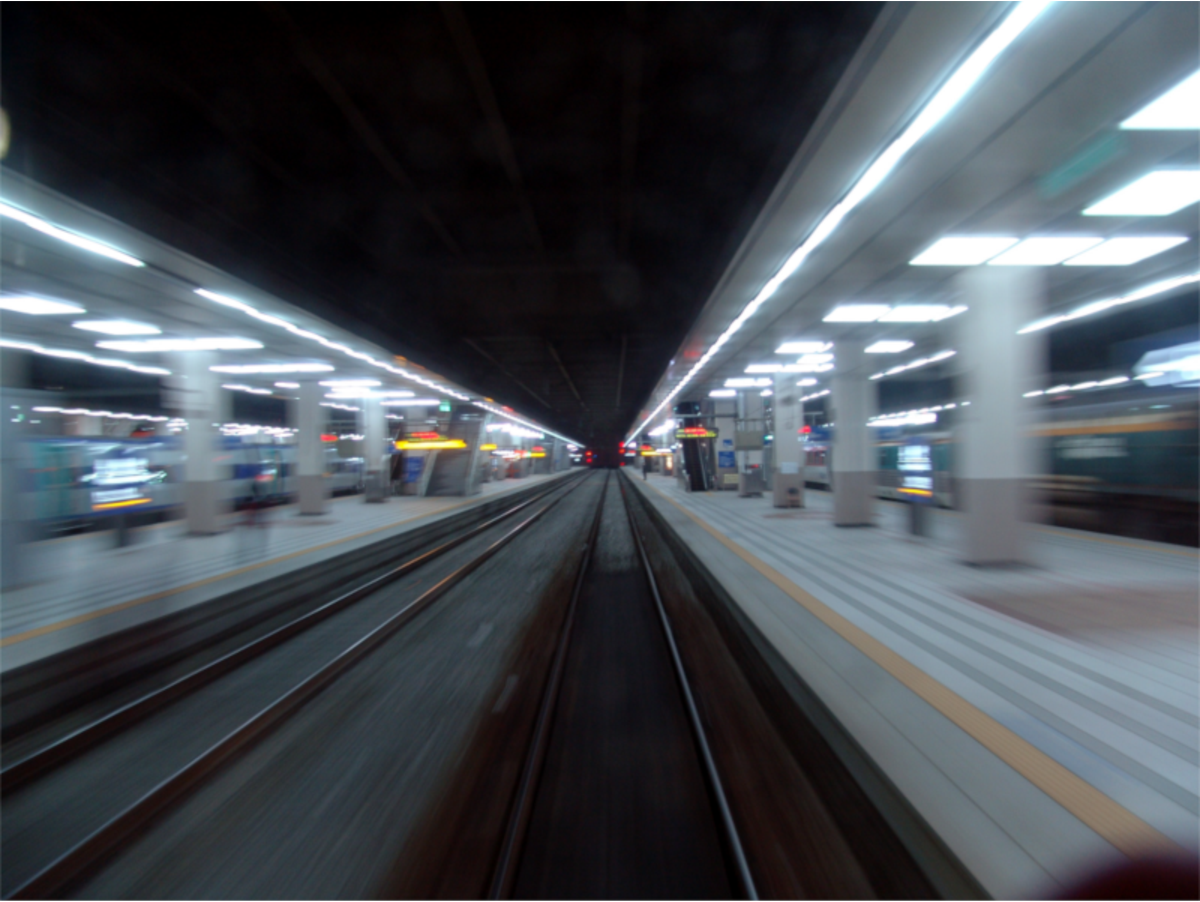
\includegraphics[width=7.5cm]{img/yongsan.pdf}}
  \caption{La estación Yongsan, en Seúl (Corea del Sur), fotografiada desde un tren. ¿Se mueve el tren o se mueve la estación? (Fuente: Wikimedia Commons - CC--BY-SA 3.0)}
\end{floatingfigure}

{\small{
  {\it Dos amigos viajan en el rápido de Buenos Aires a Rosario. Uno de ellos dice:}
  
  --¿En qué estará pensando ese señor que desde que salimos de Buenos Aires mira por la ventanilla y no se ha movido para nada?
  
  {\it El otro es un físico. Siente gusto por la discusión, por las definiciones precisas y un poco también por las bromas. Le responde:}
  
  --¿Cómo que no se ha movido? ¡Lleva recorridos unos 30 kilómetros a razón de 100 kilómetros por hora!
  
  --¡Vamos! Quiero decir que {\bf él} no se ha movido, que desde que empezó el viaje ha estado clavado en su asiento, mirando por la ventanilla, sin moverse una sola vez para nada. ¿Está claro?
  
  --No te exaltes. Más bien deberías avergonzarte de emplear las palabras tan a la ligera.
  
  --No entiendo...
  
  --Esto de hablar de moverse o no moverse es cosa peligrosa; las palabras deben emplearse con sumo cuidado. En primer lugar, fíjate que la discusión empezó porque olvidaste decir algo muy, pero muy importante.
  
  --Te olvidaste de aclarar {\bf con respecto a qué}, oye bien, con respecto a qué ese señor no se había movido. Reflexiona, que ese detalle es de importancia decisiva. En efecto: el señor no se ha movido respecto del vagón, con relación al vagón, a su asiento, a la ventanilla, si quieres. Pero en cambio se ha movido ¡y de qué manera! con relación a la ciudad de Buenos Aires. Se ha movido por lo menos 30 kilómetros, o ya 34, porque esta discusión debe llevar ya unos 4 kilómetros, si mi reloj y mi ojo no me engañan.
  
  --¡Bah! Todo eso son sutilezas y afán de discutir porque sí. No me vas a decir que toda esa palabrería tiene importancia.
  
  --¡Cuidado! Muchos grandes descubrimientos de la Física fueron hechos gracias a análisis como este, que tú calificas de palabrería. ¡Si supieras lo que Galileo, Newton y Einstein aprovecharon de discusiones así...!
  
  --Bien, señor profesor, gracias por la lección. ¿Quiere decirme, entonces, de qué manera hay que expresarse para no suscitar las iras de físicos o ingenieros o astrónomos?
  
  --No tengo inconveniente alguno. Más todavía: estoy dispuesto a confesar que experimentaré un gran placer, pero con la condición de que respondas cada vez que te haga una pregunta. Te quiero probar que tú mismo eres capaz de sacar consecuencias interesantes.
  
  --A ver...

  --Primero, supongamos que estás en el andén de una estación, adonde has ido para despedir a tu familia. ¿Cómo sabes que el tren se pone en movimiento?
   
  --Pues, porque veo que las ruedas empiezan a moverse.
   
  --No hay necesidad de ver las ruedas. Eso es lo importante. Además, las ruedas podrían girar y patinar en el mismo lugar, de modo que el tren quedaría todavía en reposo.
   
  --Pues… simplemente porque se aleja.
   
  --Estamos de acuerdo, pero si agregas un detalle ¿Se aleja de quién? ¿Respecto de qué? ¿Con relación a qué?
   
  --Pues, porque se aleja de mí, con respecto a mí, con relación a mí.
   
  --Muy bien; progresas. Veamos si eres capaz, ahora, de decirme cuándo un cuerpo cualquiera está en movimiento.
   
  --Muy sencillo. Un cuerpo está en movimiento cuando aumenta su distancia respecto de un hombre que está en un lugar.
   
  --Bastante bien, pero con dos defectos.
   
  --¿Cuáles son?
   
  --Primer defecto: según tu definición, el tren se movería cuando se va, pero no cuando viene.
   
  --Me olvidé, claro. Habría que decir ``cuando {\bf aumenta} o {\bf disminuye} su distancia''.
   
  --Sí. Pero ahora viene el segundo defecto. Según tu definición, el tren sólo se mueve si hay un hombre parado en la estación. ¿Y si no hubiera nadie, el tren no se movería lo mismo?
   
  --Bueno, claro que no es necesario que haya un hombre allí.
   
  --Entonces, ¿cómo te parece que sería correcto decir?
   
  --Un cuerpo está en movimiento cuando aumenta o disminuye su distancia respecto de un punto fijo.
   
  --Muy bien, bastante bien para un aficionado. Fíjate, sin embargo, que el problema no queda todavía resuelto. Hay mucho que hablar.
   
  --¡Cómo! ¿Todavía?
   
  --Ya lo creo. Queda algo muy importante, de enorme importancia. ¿Quién se mueve, el tren o la estación?
   
  --¡Estás bromeando…!
   
  --Hablo en serio.
   
  --No sé adónde quieres ir a parar con esa pregunta de locos, pero te responderé como si fuera una pregunta cuerda. Es el tren el que se mueve.
   
  --Así que la estación está en reposo, ¿no?
   
  --Por supuesto.
   
  --¿Y no se te ha ocurrido pensar que la estación instalada en un planeta que se mueve vertiginosamente por los espacios siderales?

   {\it Aquí el amigo del físico se llevó la mano derecha al mentón, frunció el entrecejo, reflexionó, y finalmente dijo, casi con pavor:}
   
  --¡Caramba! Me parece que lo mejor en la vida sería no pronunciar ni una sola palabra. Creo que todo es terriblemente difícil. Me acabas de hacer ver algo increíble... En efecto… Claro... Entonces, si la estación está sobre la Tierra, y si la tierra gira y se traslada vertiginosamente en el espacio... Diablos... Es la misma cosa de hoy, con el señor ese y la ventanilla y la estación... Estamos como al comienzo... ¡Por el amor de Dios! ¿Me puedes decir qué es lo verdadero y qué es lo falso? ¿Quién se mueve? ¿Quién está en reposo? Ya no entiendo nada.
   
  --Ahora tienes verdadero interés; ahora no estás fastidiado por la palabrería, ¿no es así?
   
  --Lo confieso. Me muero de curiosidad.
   
  --Muy bien. Como decía un filósofo griego, el asombro es la madre de la sabiduría. Hay que empezar por asombrarse y preguntar, como los chicos: ¿por qué?, ¿por qué?
   
  --Bueno; responde de una buena vez.
   
  --Pues, en cierto modo, la respuesta es muy simple. Todos los movimientos son relativos, es decir, {\bf con relación a algo}, a un punto. Por ejemplo, para empezar con nuestro señor, el que originó la discusión, ese señor, está en reposo con relación al vagón, pero también podemos invertir la frase diciendo que el vagón está en reposo respecto al señor. Pero ese señor está en movimiento con respecto a la estación...
   
  --¿De modo que alguien o algo puede estar {\bf a la vez en reposo y en movimiento}?
   
  --Exacto. Todo depende del punto de referencia que se elija como fijo. Como decía, ese señor se mueve respecto a ese señor, considerándolo a él como fijo. No hay más derecho a decir lo primero que lo segundo, pues la estación no es ningún ente privilegiado, ya que pierde inmediatamente su jerarquía o su importancia en cuanto pensamos en el Sol o las estrellas. ¿Acaso la estación está en reposo respecto del Sol? De ningún modo.
   
  --¿Entonces?
   
  --Entonces, si queremos ser verídicos y no decir más que lo que debemos decir, habrá que definir el movimiento de esta manera...
   
  --Un momento, intentaré hacerlo yo.
   
  --Veamos...
   
  --Yo diría que ``un cuerpo está en movimiento con relación a un punto elegido como fijo, cuando aumenta o disminuye su distancia respecto a ese punto''.
   
  --¡Magnífico! Se puede todavía hacer una simplificación. En Física hay que emplear siempre el mínimo de palabras, y acá sobran dos.
   
  --A ver... ¡Ya sé!: {\bf ``Un cuerpo está en movimiento con relación a un punto elegido como fijo, cuando varía su distancia a ese punto''}.
   
  --Muy bien. Ahora tú mismo puedes extraer algunas conclusiones bastante curiosas sobre fenómenos que son bien conocidos. ¿Qué me podrías decir sobre dos trenes expresos que corren uno al lado del otro, en la misma dirección, el mismo sentido y con la misma velocidad?
   
  --Que un tren está en reposo con respecto al otro.
   
  --Perfecto. ¿Qué me podrías decir si uno de esos trenes se mueve a 100 kilómetros por hora y el otro a 90?
   
  --Que el primero se mueve a 10 kilómetros por hora con relación al segundo.
   
  --¡Magnífico! Creo que la lección ha sido provechosa. Puede sentarse, joven. Le pondré diez puntos.
   
  --¡Un momento, señor profesor! Me parece que la definición que usted acepta tiene un defecto.
   
  --¡Esto sí que está bueno! Así es, tiene un defecto. Si has dado en el clavo, resultarás mejor alumno de lo que yo esperaba. ¿Cuál es el defecto?
   
  --¿Qué pasa si revoleo una piedra y elijo como punto fijo mi hombro? La piedra recorre una circunferencia cuyo centro es mi hombro. La distancia de la piedra a mi hombro no varía, y sin embargo, la piedra se mueve.
   
  --Ese es el defecto. Para definir el movimiento con toda precisión, debe elegir no un punto de referencia, sino un {\bf sistema de referencia}. Pero, ¿recuerdas lo que es sistema de referencia?
   
  --Sí... tres rectas que se cortan en un mismo punto.
   
  --Y cada una perpendicular a las otras dos. Como las aristas de las paredes de una habitación que concurren a un mismo rincón. Y ahora, en lugar de decir: “Un cuerpo está en movimiento con relación a un punto cuando varía su distancia respecto de ese punto...”
   
  --Déjamelo decir a mí: ``Un cuerpo está en movimiento con relación a un sistema de referencia, elegido como fijo, cuando varían... ¡sus coordenadas en ese sistema!''
   
  --Bueno, hombre ahora tendría que ponerte diez y felicitarte...

  \bigskip
   \begin{flushright}
  {   \small{\it Texto adaptado del libro ``Física 1'' de Maiztegui y Sábato (2da ed. Kapeluz, 2005).}}
\end{flushright}
}}


\defin{Movimiento}

{\bf Un cuerpo está en movimiento con relación a un sistema de referencia elegido como fijo, cuando sus coordenadas en ese sistema varían a medida que transcurre el tiempo.}


\defin{Sistema de referencia}

Para describir un movimiento, un {\bf observador} elige un objeto o un conjunto de objetos que considera {\bf fijos} y allí coloca un conjunto de ejes de coordenadas. Este conjunto de ejes de coordenadas, {\bf en reposo con respecto al observador}, es lo que denominamos {\bf sistema de referencia}.

El concepto de movimiento se refiere a la modificación de la posición relativa de los cuerpos entre sí, por eso es necesario definir un sistema de referencia.
\begin{center}
  
\includegraphics[scale=1.2]{img/movimiento.pdf}
\end{center}

El sistema de referencia tiene tanta importancia que no podemos hablar de reposo o de movimiento si no hablamos simultáneamente del sistema de referencia a partir del cual tenemos esa condición de reposo o de movimiento.

{\bf El sistema de referencia} es arbitrario y puede ser elegido por el observador de la forma que lo crea más conveniente para la descripción del movimiento que esté estudiando, {\bf pero una vez seleccionado debe ser mantenido invariable}.


\begin{figure}[H]
\centering
\begin{minipage}{.4\textwidth}
  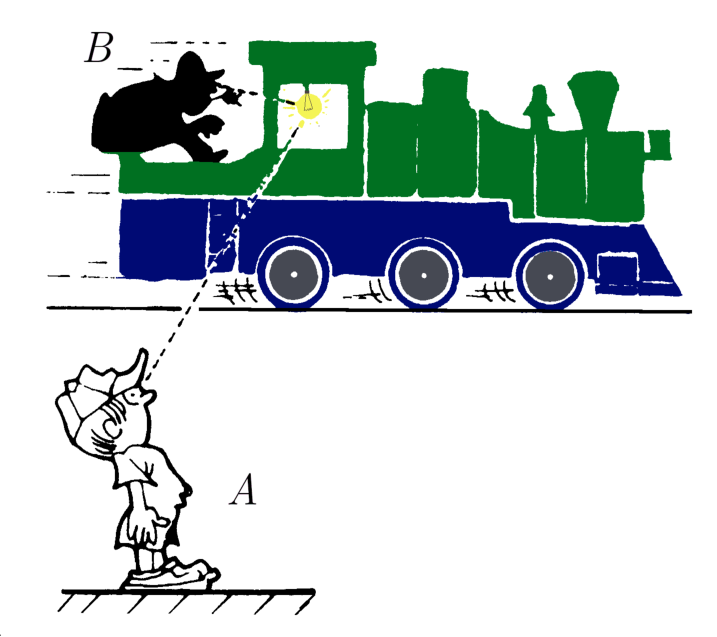
\includegraphics[width=\textwidth]{img/tren.pdf}
  \caption{La lámpara está inmóvil en relación con el observador $B$, pero se encuentra en movimiento en relación con el $A$.}
\end{minipage}%
\hfill
\begin{minipage}{.55\textwidth}
  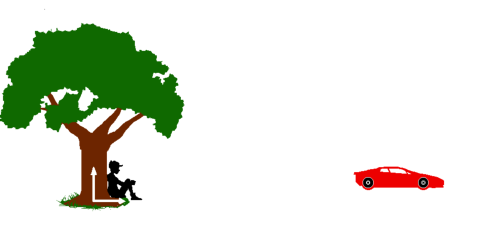
\includegraphics[width=\textwidth]{img/arbol.pdf}
  \caption{En la figura se ve un observador que ve alejarse un auto, ha elegido un sistema de  referencia (el árbol) y en él ha fijado un sistema de coordenadas, en este caso un sistema de ejes ortogonales.}
\end{minipage}
\end{figure}
    
\begin{comprension}
Retomando el ejemplo del tren: elige distintos sistemas de referencia y determina para cada uno qué cuerpos se mueven y qué cuerpos permanecen en reposo: persona parada en el andén de la estación, tren en marcha, persona sentada en el tren, persona caminando por el pasillo del ómnibus.
\end{comprension}


\defin{Partícula}

Un auto que se mueve por una autopista experimenta un movimiento de traslación, sus ruedas tienen un movimiento rototraslacional y además existe un movimiento vibratorio en todas sus partes.

En esta Unidad, abordaremos sólo el movimiento traslacional y específicamente el movimiento rectilíneo de partículas. Pero, ¿qué es una partícula?

Llamamos {\bf cuerpo puntual} o {\bf partícula} a todo cuerpo cuyas dimensiones son despreciables frente a las distancias que recorre. 

Por ejemplo, la Tierra puede ser considerada partícula en su movimiento orbital como planeta, puesto que la distancia Tierra--Sol es muchas veces mayor que el radio terrestre. En cambio, no puede ser considerada partícula cuando se estudian fenómenos como las mareas o los terremotos o cuando se examina su estructura interna.
En una escala mucho más pequeña, es posible explicar la presión ejercida por un gas sobre las paredes de un recipiente considerando las moléculas de gas como partículas, por otro lado no las podemos considerar partículas cuando se estudian propiedades que dependen de la rotación y vibración molecular. 

Vamos a trabajar, por ahora, con el {\bf \color{NavyBlue} modelo de partícula}. Con este modelo a los cuerpos los representamos por puntos.

\begin{comprension}
Piensa en un cuerpo cualquiera y menciona un ejemplo en el que se lo pueda considerar partícula y otro en el que no se pueda.
\end{comprension}

\defin{Trayectoria}

{\bf Conjunto de puntos del espacio que ocupa la partícula a lo largo de su movimiento.}

Un ejemplo de trayectoria es la ``línea dibujada'' por una abeja al volar por el jardín. Esta es una trayectoria muy complicada, como lo es también la trayectoria de una pelota durante un partido de fútbol.

Si la trayectoria es una curva, el movimiento es curvilíneo. Existen muchos movimientos curvilíneos diferentes, entre ellos podemos mencionar, en particular, los movimientos circulares y los parabólicos.

Si la trayectoria está contenida en una línea recta, {\bf el movimiento es  rectilíneo}.



\begin{figure}[!h]
\centering
\begin{minipage}{.55\textwidth}
  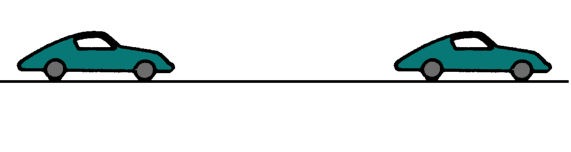
\includegraphics[width=\textwidth]{img/tray_rect.pdf}
  \caption{Una trayectoria rectilínea}
\end{minipage}%
\hfill
\begin{minipage}{.4\textwidth}
  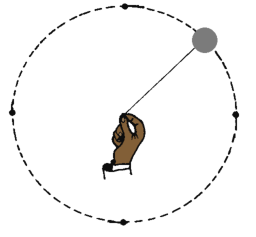
\includegraphics[width=\textwidth]{img/tray_curv.pdf}
  \caption{Una trayectoria curvilínea y circular}
\end{minipage}
\end{figure}

{\color{NavyBlue} \bf En este capítulo nos limitaremos a estudiar los movimientos cuya trayectoria es rectilínea.}

{\bf Para estudiar los movimientos rectilíneos, asociaremos al sistema de referencia un sistema de coordenadas que consiste en una recta que contiene a la trayectoria. En esta recta se indicará el origen $O$ y además se le asignará un sentido. Este sentido estará determinado por el signo positivo para una de las dos semirrectas que quedan determinadas por $O$.}


%% Acá va la parte de velocidad que escribió Gabi.
% \documentclass[a4paper, 12pt, usenames]{report}

% \usepackage[spanish]{babel}
% \usepackage[utf8]{inputenc}
% \usepackage{graphicx}
% \usepackage{caption}
% \usepackage{subcaption}
% %\usepackage{subfigure}
% \usepackage{wrapfig}
% \usepackage{bbding} %Fuentes con iconos lindos

% \usepackage[rflt]{floatflt} %Para meter figuras flotantes entre el texto
% \usepackage[font=footnotesize,labelfont=bf]{caption}
% \usepackage[dvipsnames]{xcolor}
% \usepackage{bclogo} %Iconos bonitos hechos con tikz
% \usepackage{parskip}
% \usepackage{fixmath}

% \usepackage{flushend}

% \usepackage{amsmath}


% \newcommand{\defin}[1]{\bigskip{\large  \color{Orange} \PencilRightDown{} \bf {#1}} }
% \newcommand{\ejerc}[1]{\bigskip{\color{OliveGreen} \FourClowerSolid{} {\bf Ejercitemos nuestra comprensión:}}

%   \vspace*{-0.5\baselineskip}
%   \noindent
%   \rule{17cm}{.5pt}
% #1

% \vspace*{-0.5\baselineskip}
% \noindent
% \rule{17cm}{.5pt}
% \vspace*{-0.5\baselineskip}
% }

% \newcommand{\info}[1]{
% \begin{itemize}
% \item[\bcinfo] {\footnotesize {#1}}
% \end{itemize}
% }

% \topmargin=-2.5cm
% \oddsidemargin=-0.5cm
% \textheight=25cm
% \textwidth=17cm


% \begin{document}



\defin{Posición}

Dar la posición de un cuerpo puntual significa ubicar el punto unívocamente respecto del sistema de coordenadas. Observemos dos ejemplos, en el espacio y en el plano.


\begin{figure}[H]
\centering
\begin{minipage}{.45\textwidth}
\center
  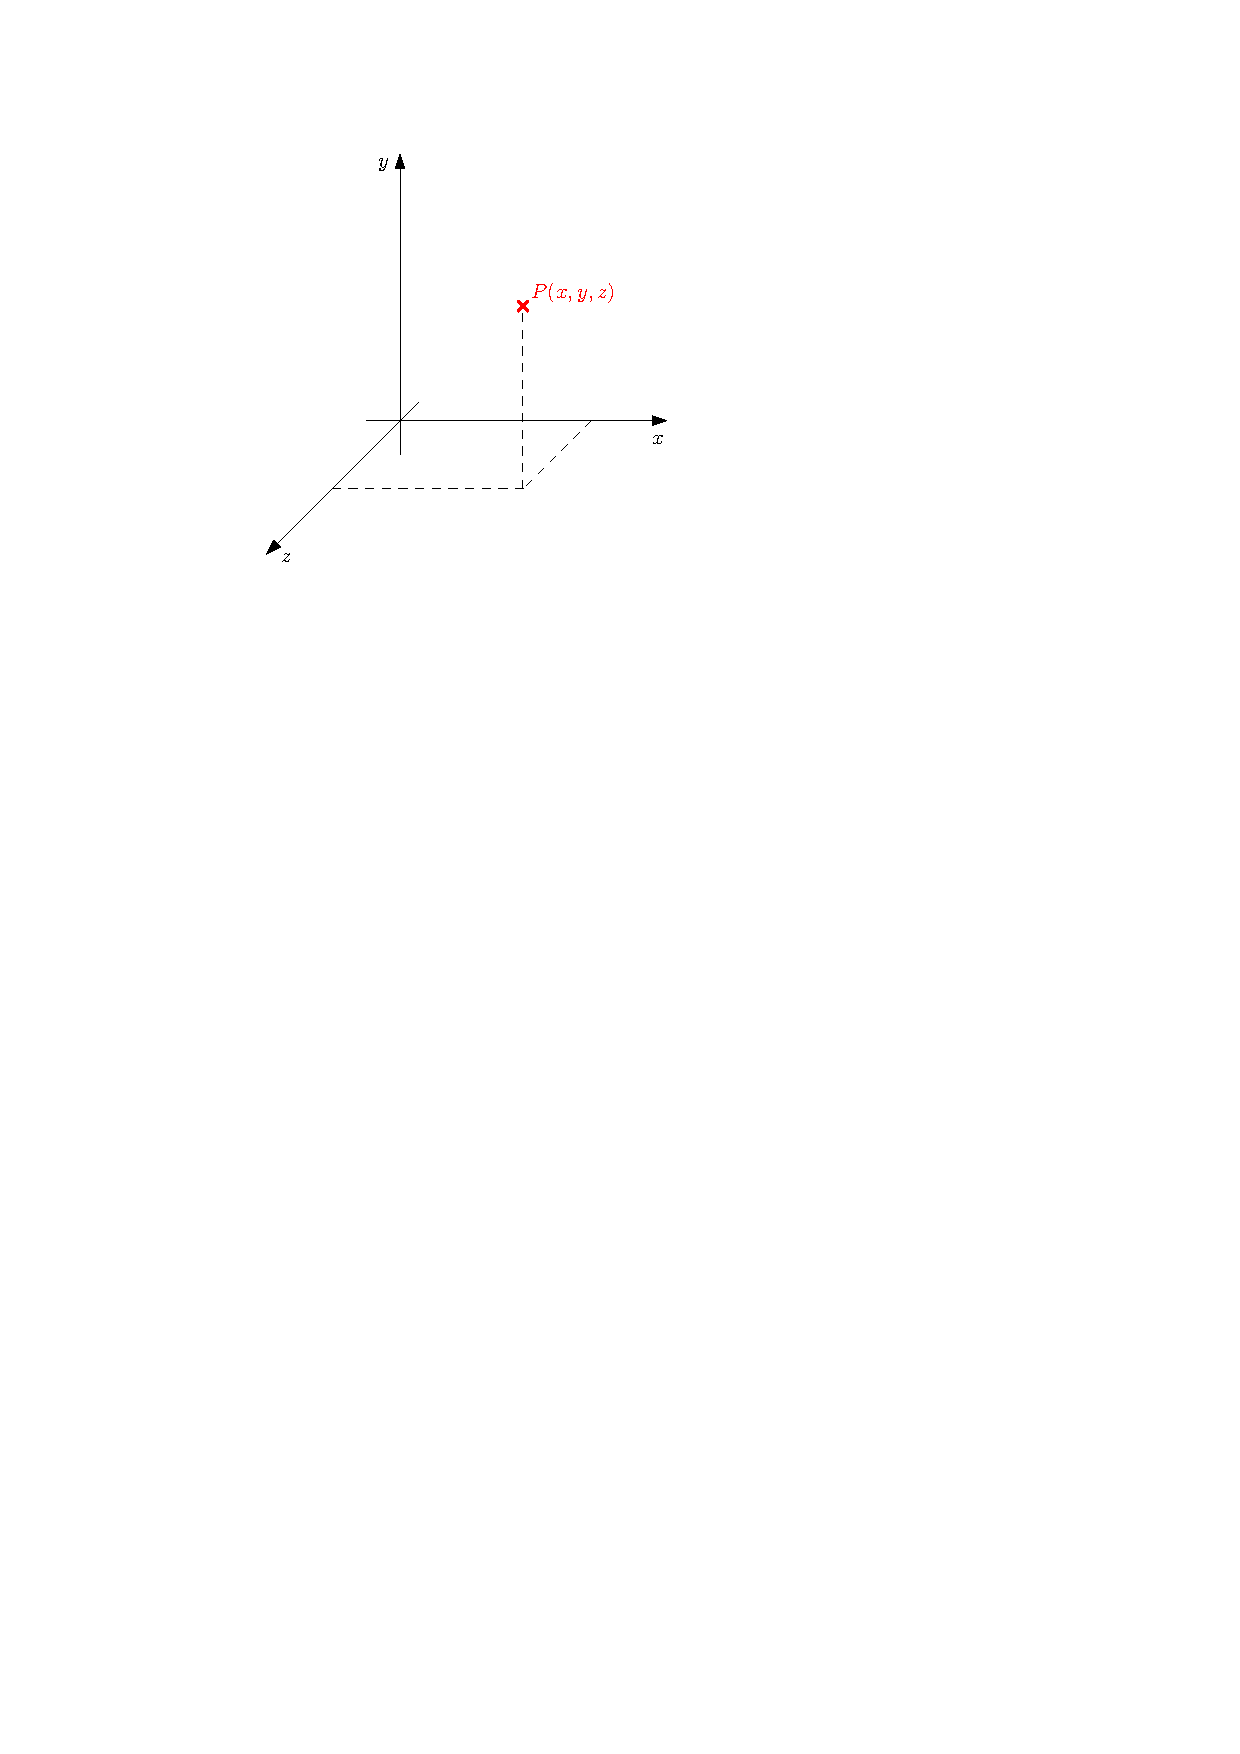
\includegraphics[width=.9\textwidth]{img/3d.pdf}
  \caption{Posición en el espacio.}
\end{minipage}%
\hfill
\begin{minipage}{.45\textwidth}
\center
  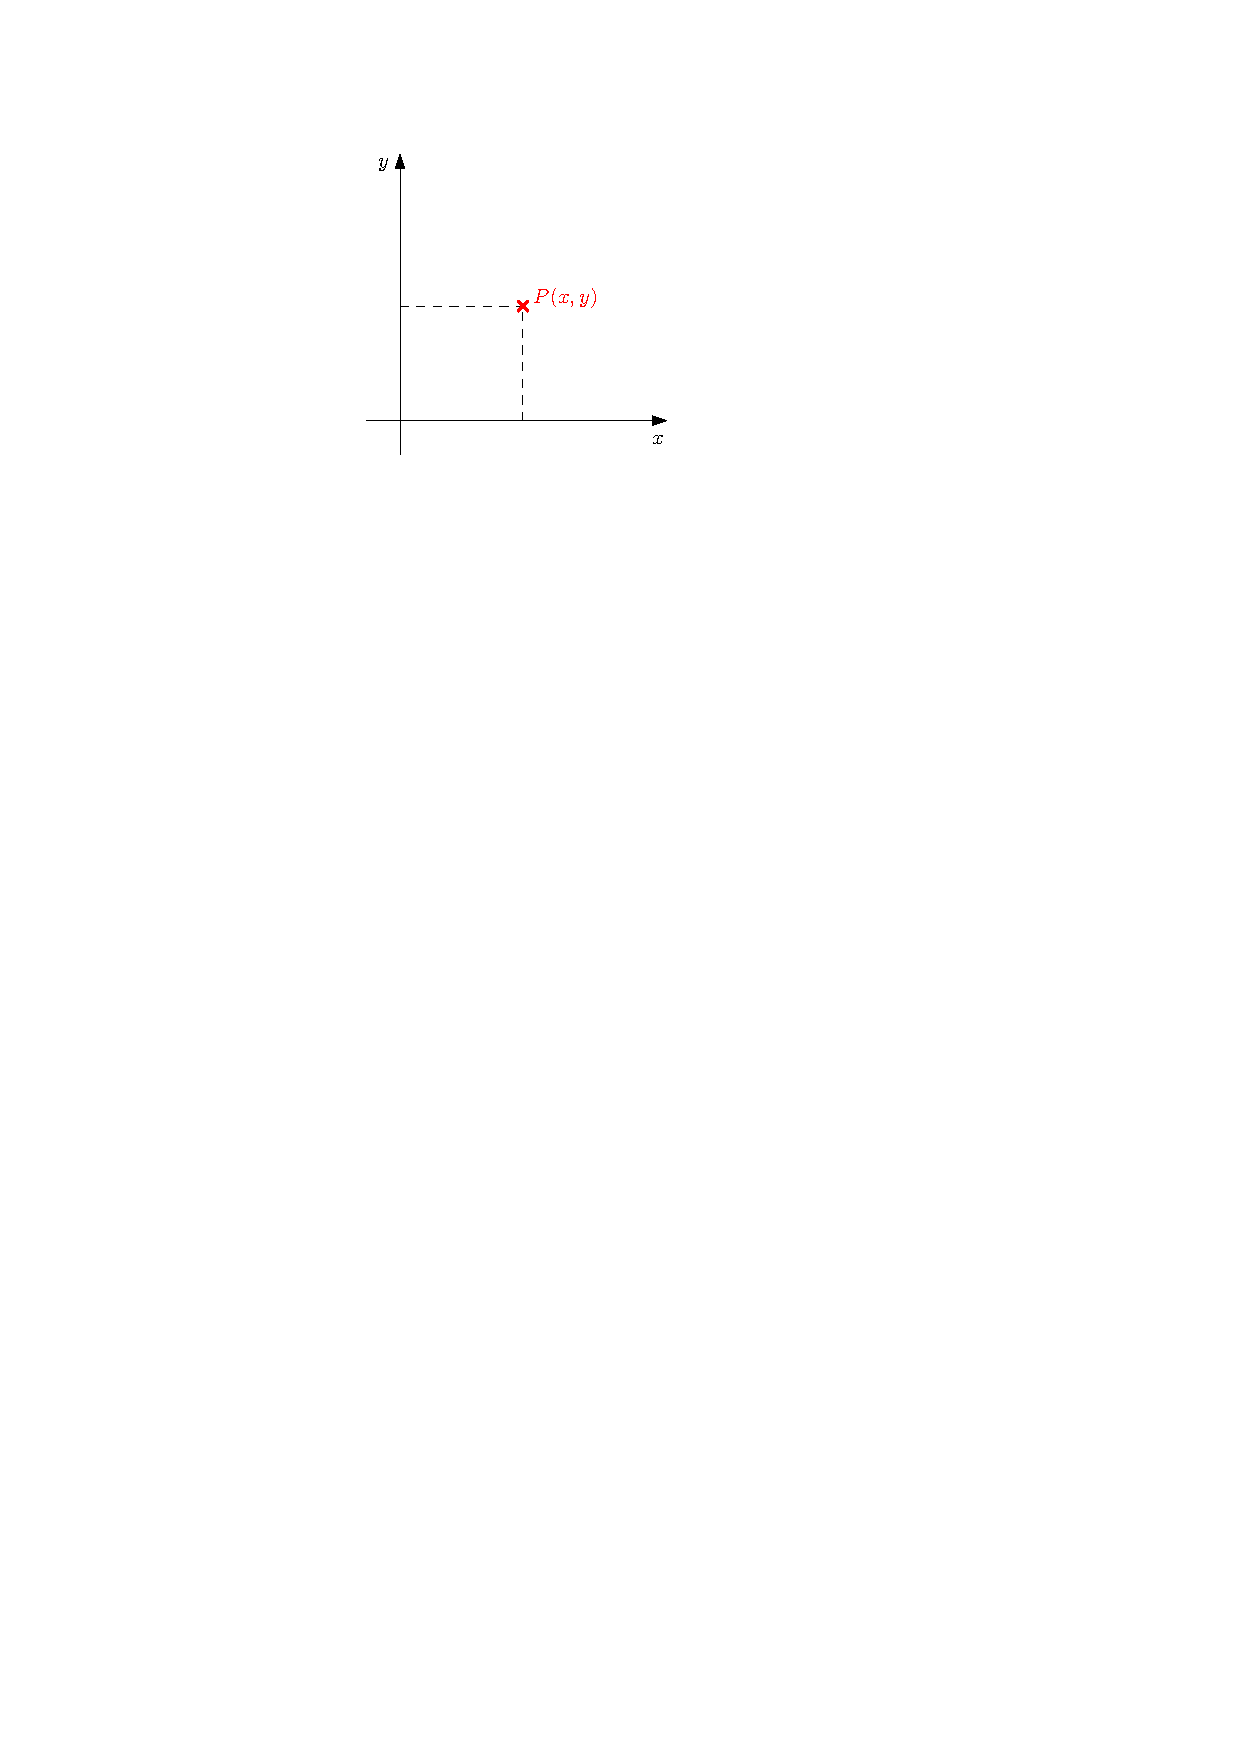
\includegraphics[width=.9\textwidth]{img/2d.pdf}
  \caption{Posición en el plano.}
\end{minipage}
\end{figure}


En los movimientos rectilíneos, para dar la posición de una partícula, sólo necesitamos una magnitud  que represente la distancia entre un punto fijo, el origen de coordenadas, y la ubicación de la partícula. Esta magnitud queda determinada por un número y su unidad. Este número  puede ser  positivo o negativo, según la partícula se encuentre a la derecha o a la izquierda del origen de coordenadas.

\begin{figure}[H]
\center
 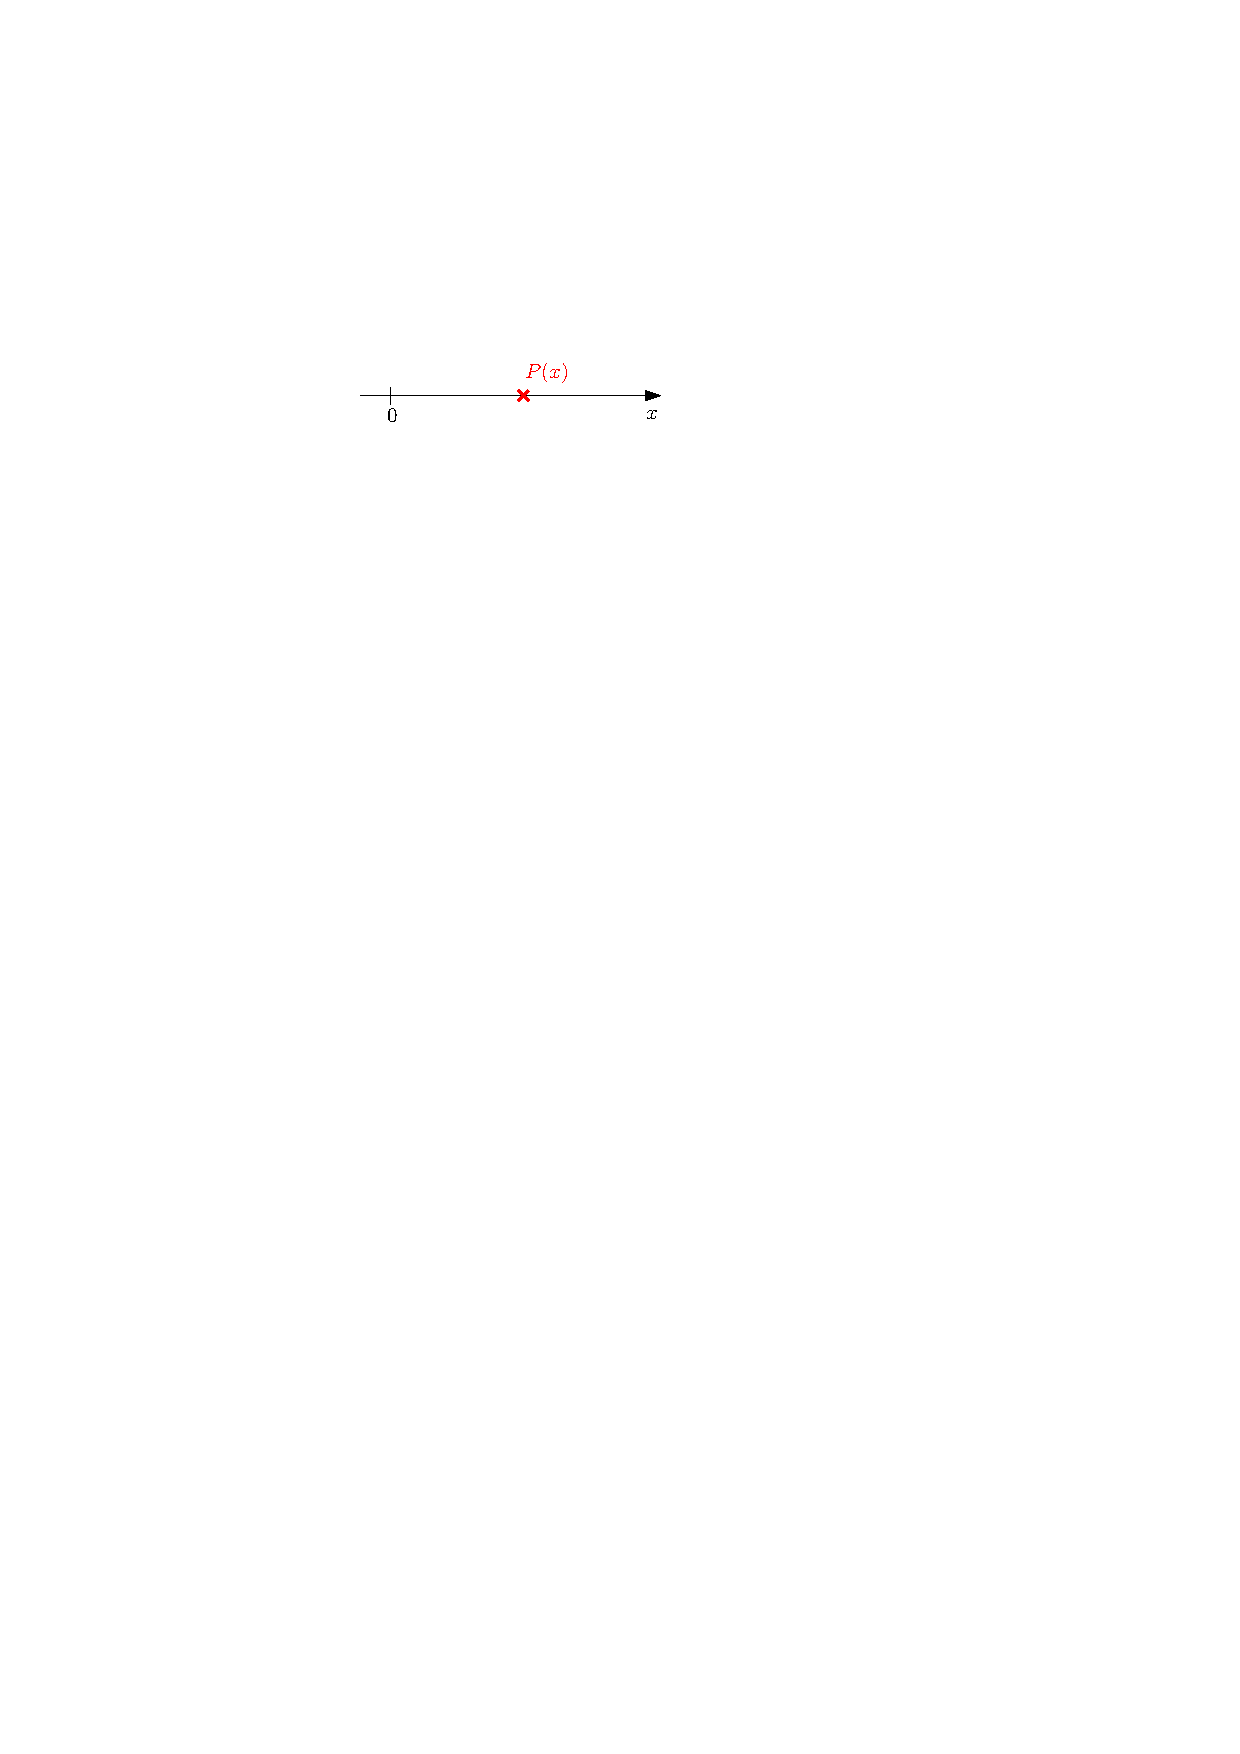
\includegraphics[width=.4\textwidth]{img/1d.pdf}
  \caption{Posición en una dimensión.}
\end{figure}


\defin{Distancia recorrida}

La distancia recorrida se refiere a la longitud de la trayectoria que recorre la partícula en un determinado intervalo de tiempo durante su movimiento.

Es una {\bf magnitud escalar}.



\defin{Desplazamiento}

Cuando una partícula se mueve desde la posición $\mathbold{P_0}$ hasta la posición $\mathbold{P}$, su desplazamiento esta dado por $\mathbold{\bar{d}}$, como observamos en la figura:


\begin{figure}[h!]
\centering
 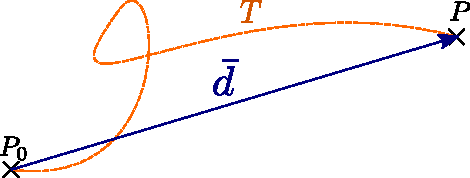
\includegraphics[width=.4\textwidth]{img/trayectoria_distancia.pdf}
  \caption{Desplazamiento de una partícula y la trayectoria de su movimiento.}
\end{figure}


Vemos, entonces, que el desplazamiento es un {\bf vector} con origen en la posición inicial de la partícula {$\mathbold{P_0}$} y extremo en la posición final de la misma {$\mathbold{P}$}. Es decir que \underline{solo} depende de la posición inicial y final de dicha partícula. 

El desplazamiento es una {\bf magnitud vectorial}.


En particular, en un movimiento rectilíneo, el desplazamiento se representa de la siguiente manera:


\begin{figure}[h!]
\centering
 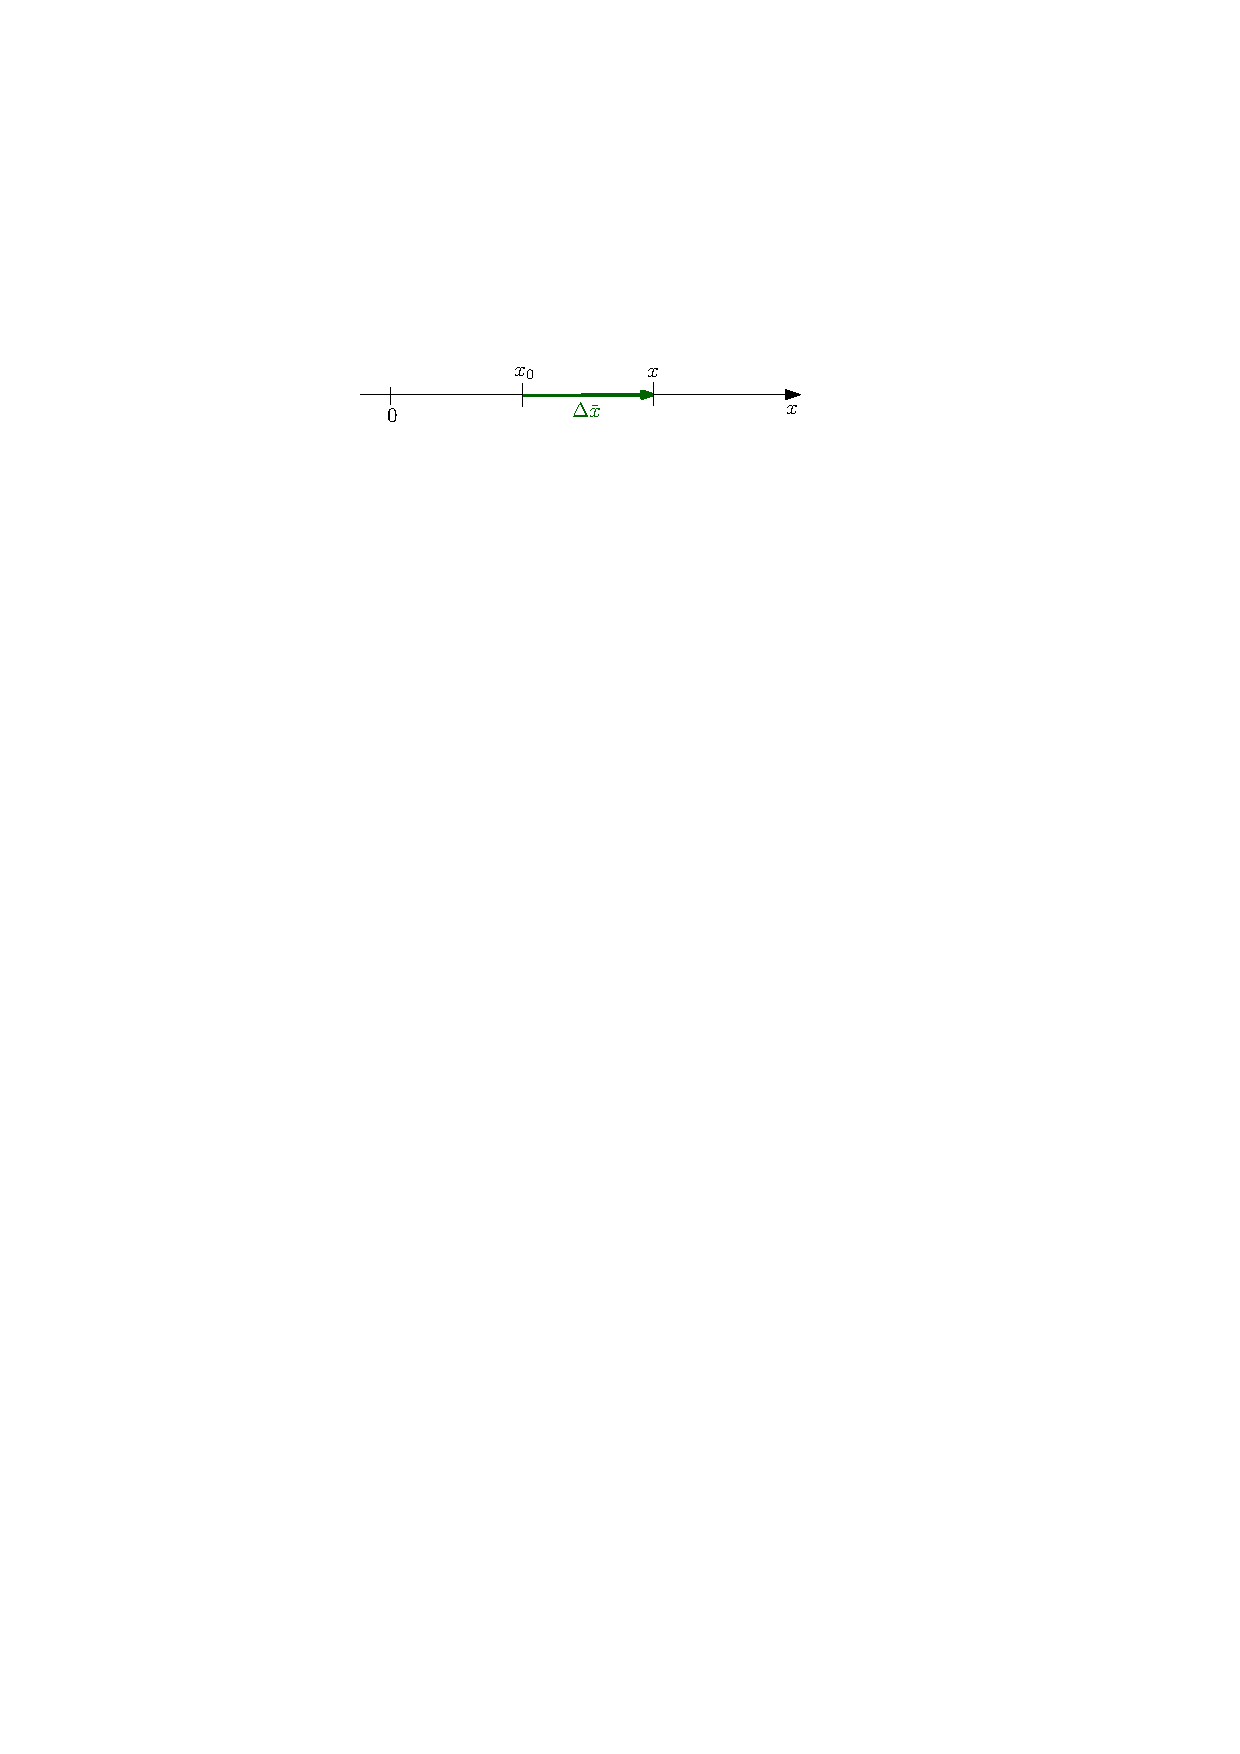
\includegraphics[width=.5\textwidth]{img/deltax.pdf}
  \caption{Desplazamiento en un movimiento rectilíneo.}
\end{figure}
en donde el {\bf módulo} del {\it vector desplazamiento} esta dado por: $$|\Delta \bar{x}| = \vert x - x_0 \vert$$

\info{En este curso, utilizaremos la letra griega $\mathbold{\Delta}$ (Delta mayúscula) para indicar {\bf \em variación}.
  Si, por ejemplo, nos encontramos con la expresión $\Delta a$, queremos decir ``el valor final de la magnitud $a$ menos su valor inicial $a_0$''. El subíndice cero siempre indicará el valor inicial de la magnitud que acompaña.}


Vamos a destacar que tanto el desplazamiento como la distancia recorrida se miden en {\bf metros (m)}, unidad base del SI y del SIMELA.
\bigskip


%%% % TABLA DE MAGNITUDES ESCALARES Y VECTORIALES

\begin{magnitud}{Magnitudes Físicas}
  En el curso anterior vimos que una magnitud quedaba definida en un proceso de medición. Teniendo en cuenta lo definido anteriormente, en este curso  necesitaremos distinguir entre dos tipos de magnitudes físicas:
  \begin{center}
  \begin{tabular}{|l|p{6cm}|p{6cm}|}
    \hline
    & Para definirlas se necesita        & Ejemplos\\
    \hline
    $\bullet$ Escalares:& $\rightarrow$ Un número real

                          $\rightarrow$ Una unidad de medida.
                          
                                         &
                                           \vspace*{-0.5\baselineskip}
                                           \begin{itemize}[leftmargin=*,nosep]
                                         \item[$\bullet$] 10\,\textordmasculine C
                                         \item[$\bullet$] 20 s
                                         \end{itemize}\\
                                           \hline
    $\bullet$ Vectoriales:& 
                            $\rightarrow$ Un vector, que consta de:
                            \begin{itemize}[nosep]
                            \item Una {\bf dirección} (recta sobre la que se encuentra)
                            \item Un {\bf sentido} (Indicado por una flecha)
                            \item Un {\bf módulo} (la medida del vector)
                            \end{itemize}
                            $\rightarrow$ Una unidad de medida.
                                         &
                                           \vspace*{-0.5\baselineskip}
                                           \begin{itemize}[leftmargin=*,nosep]
                                           \item[$\bullet$]  20 km/h en dirección Norte-Sur, hacia el Sur.
                                           \item[$\bullet$] 0,8 m en dirección vertical, hacia abajo.
                                           \end{itemize}
                                         \\
                                           
    \hline
  \end{tabular}
\end{center}
\end{magnitud}

\clearpage
\begin{comprension}
  {\bf Primero:}

Indica en los siguientes casos el desplazamiento {$\mathbold{\bar{d}}$} de una partícula que se mueve desde {$\mathbold{P_0}$} hasta {$\mathbold{P}$}:

\begin{figure}[H]
 \begin{subfigure}{0.5\textwidth}
    \centering
 	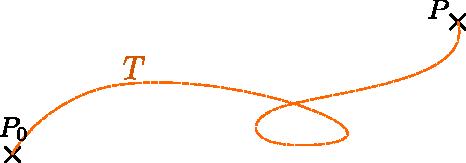
\includegraphics[width=.7\linewidth]{img/trayectoria_ej1.pdf}
	\caption{}	
\end{subfigure}   
 \begin{subfigure}{0.5\textwidth}
    \centering
 	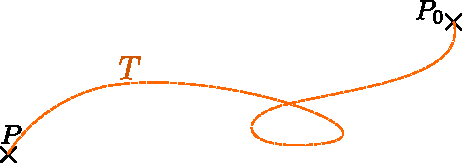
\includegraphics[width=.7\linewidth]{img/trayectoria_ej2.pdf}
	\caption{}	
\end{subfigure} 
 \begin{subfigure}{0.5\textwidth}
    \centering
 	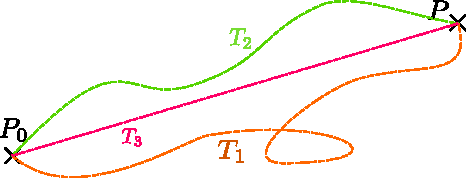
\includegraphics[width=.7\linewidth]{img/trayectoria_ej3.pdf}
	\caption{}	
\end{subfigure} 
 \begin{subfigure}{0.5\textwidth}
    \centering
 	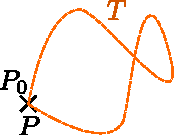
\includegraphics[width=.35\linewidth]{img/trayectoria_ej4.pdf}
	\caption{}	
\end{subfigure}
\end{figure}

\noindent
{\bf Segundo:}

Indica en los siguientes casos la {\it trayectoria}, el {\it desplazamiento } ($\mathbold{\Delta \bar{x}}$) y la {\it distancia recorrida}:

\begin{figure}[H]
 \begin{subfigure}{0.5\textwidth}
    \centering
 	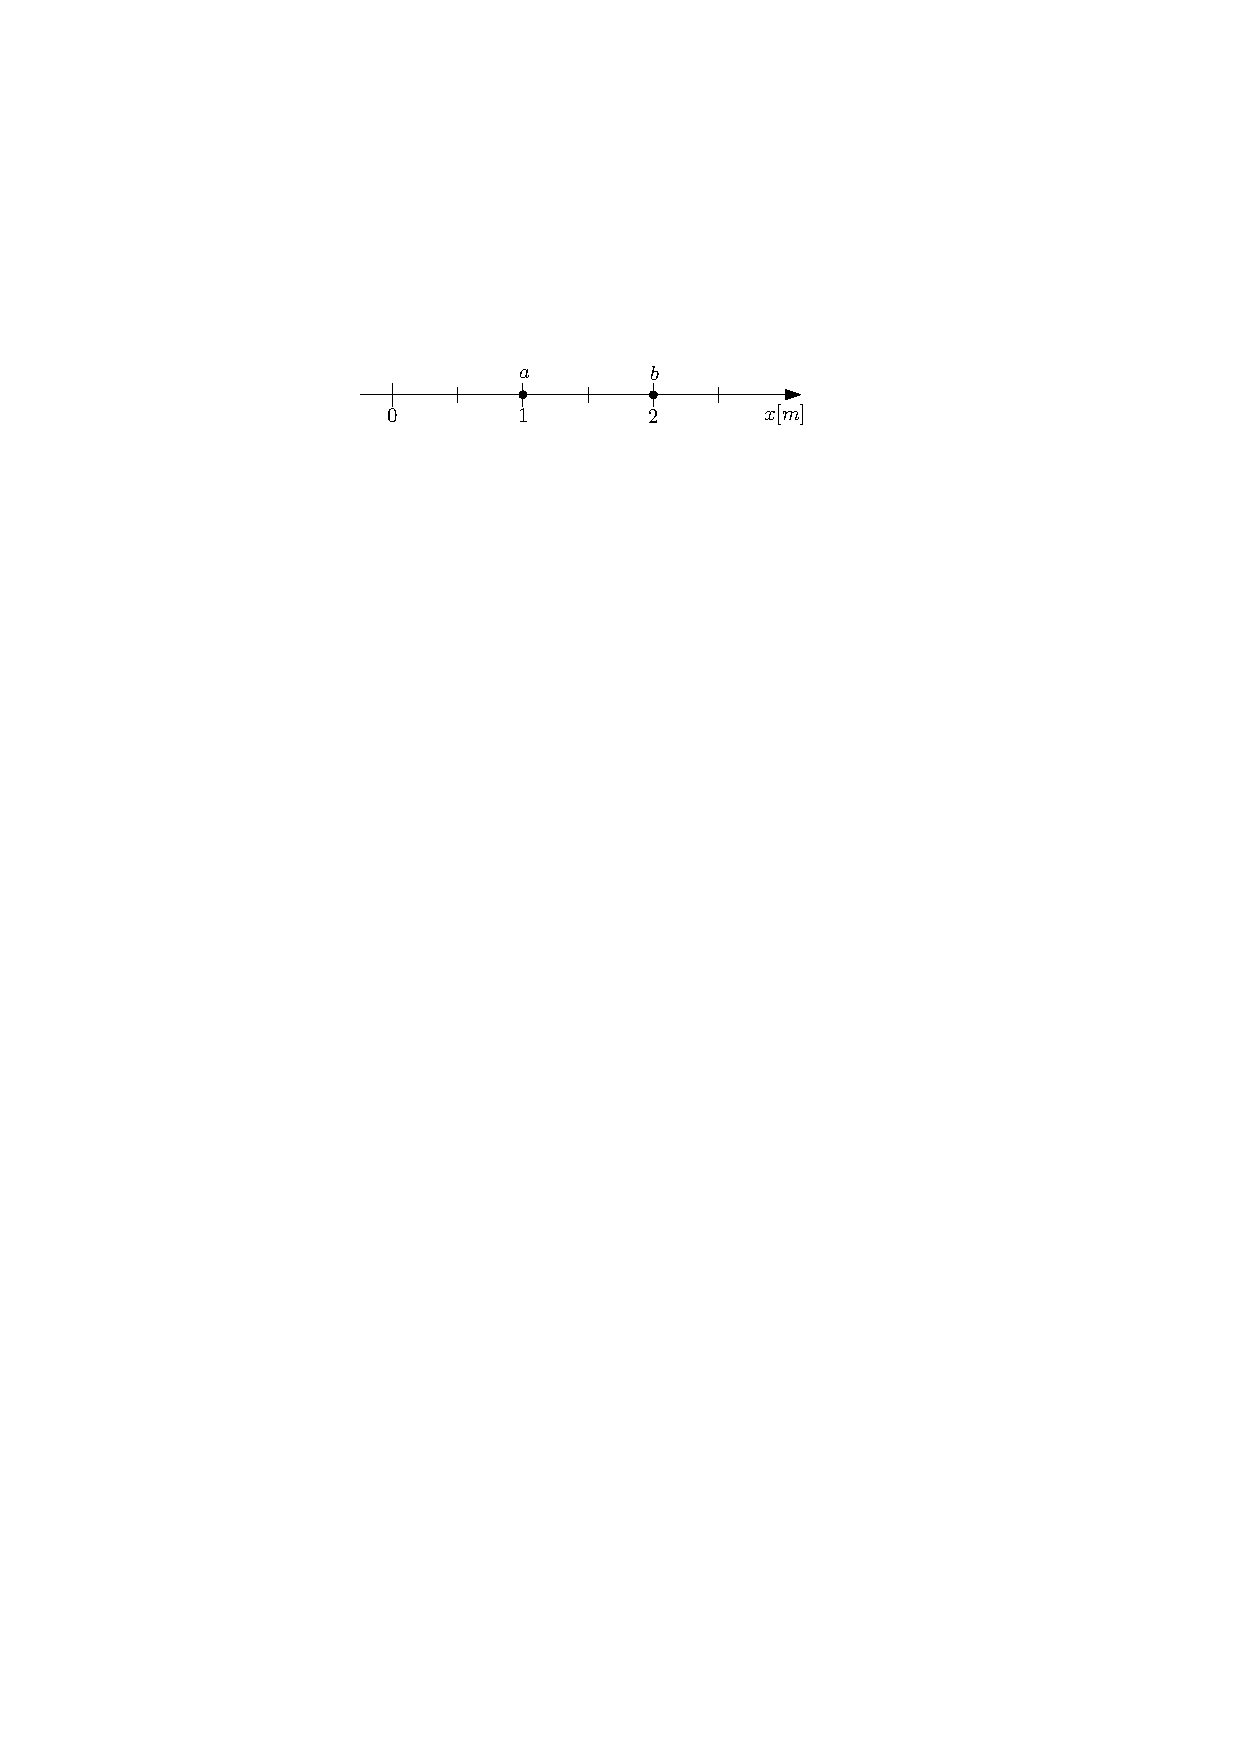
\includegraphics[width=.9\linewidth]{img/p_t_d_ej1.pdf}
	\caption{Una partícula se mueve desde $a$ hasta $b$.}	
\end{subfigure}   
 \begin{subfigure}{0.5\textwidth}
    \centering
 	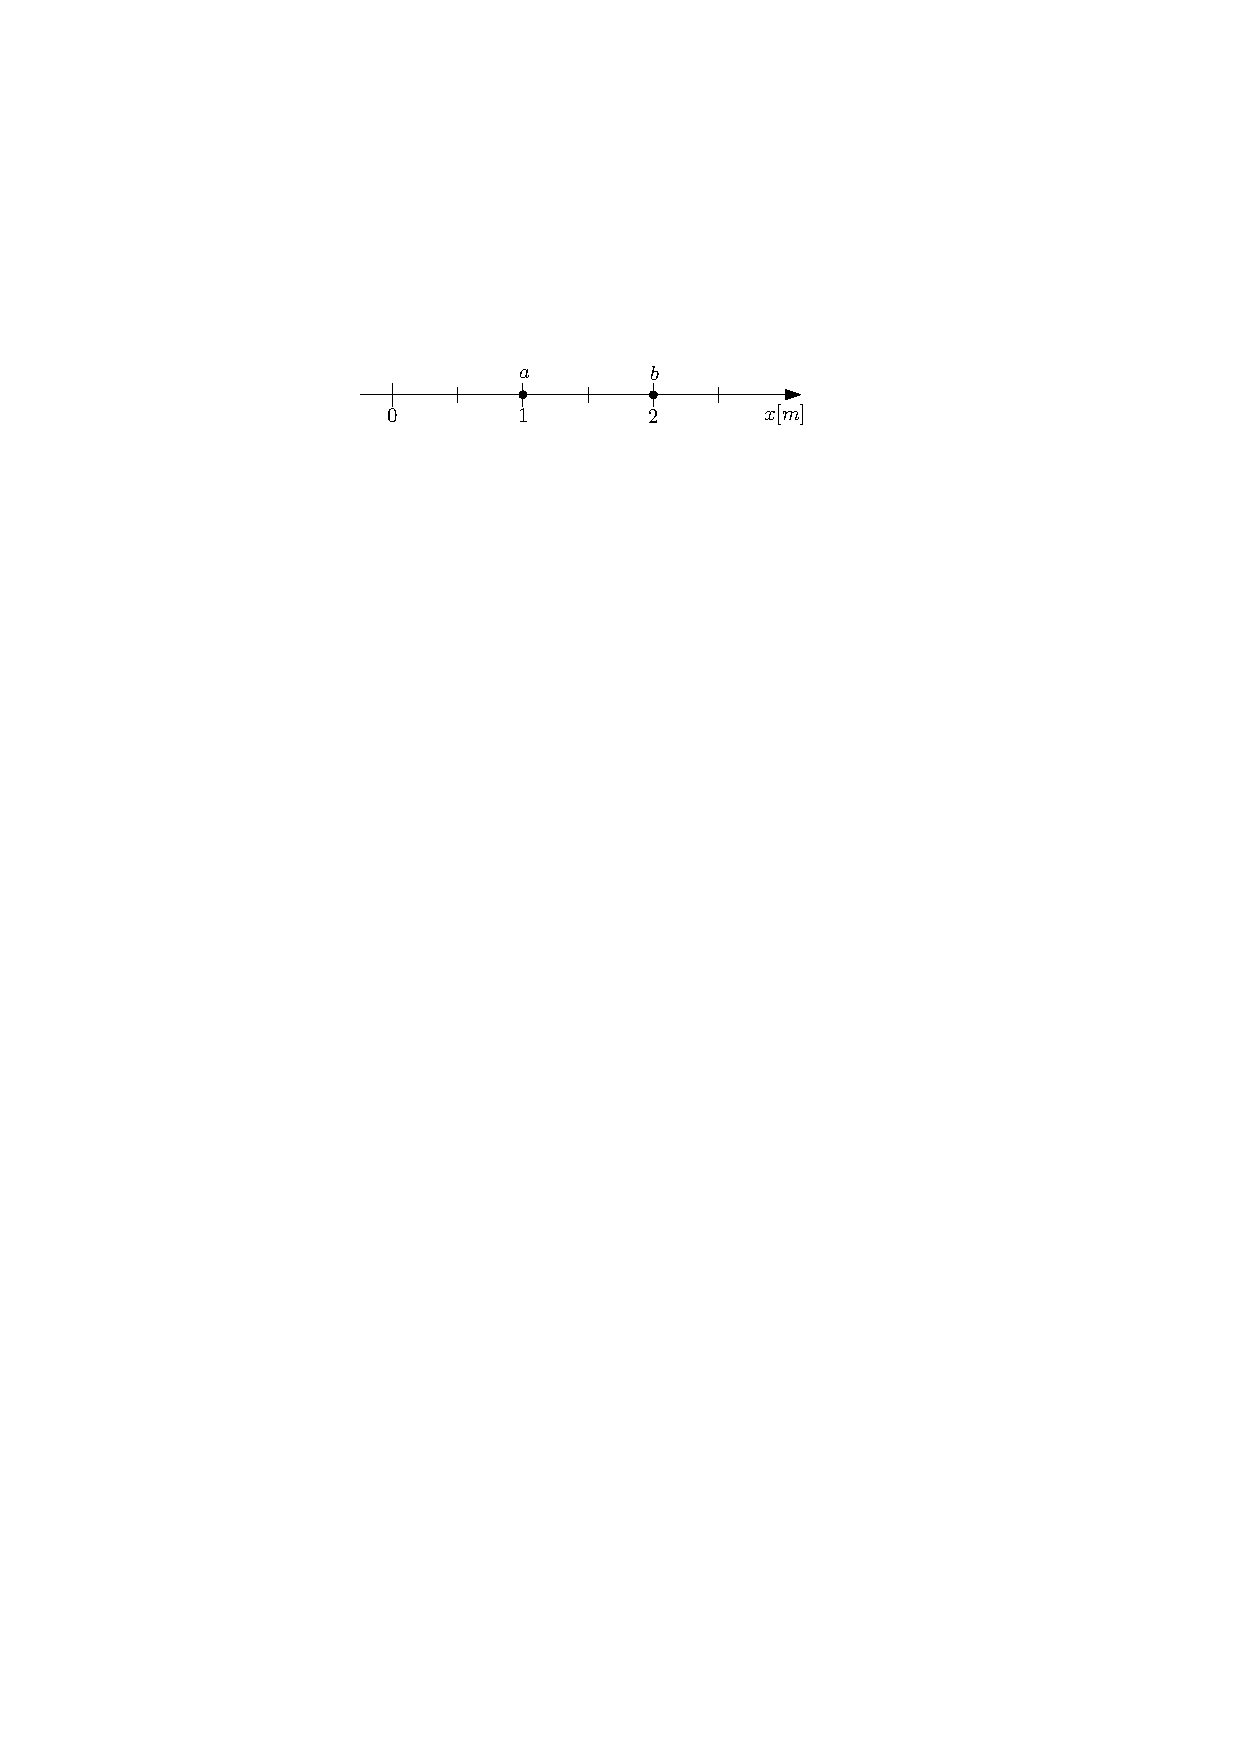
\includegraphics[width=.9\linewidth]{img/p_t_d_ej1.pdf}
	\caption{Una partícula se mueve desde $b$ hasta $a$.}	
\end{subfigure}
 \begin{subfigure}{0.5\textwidth}
    \centering
 	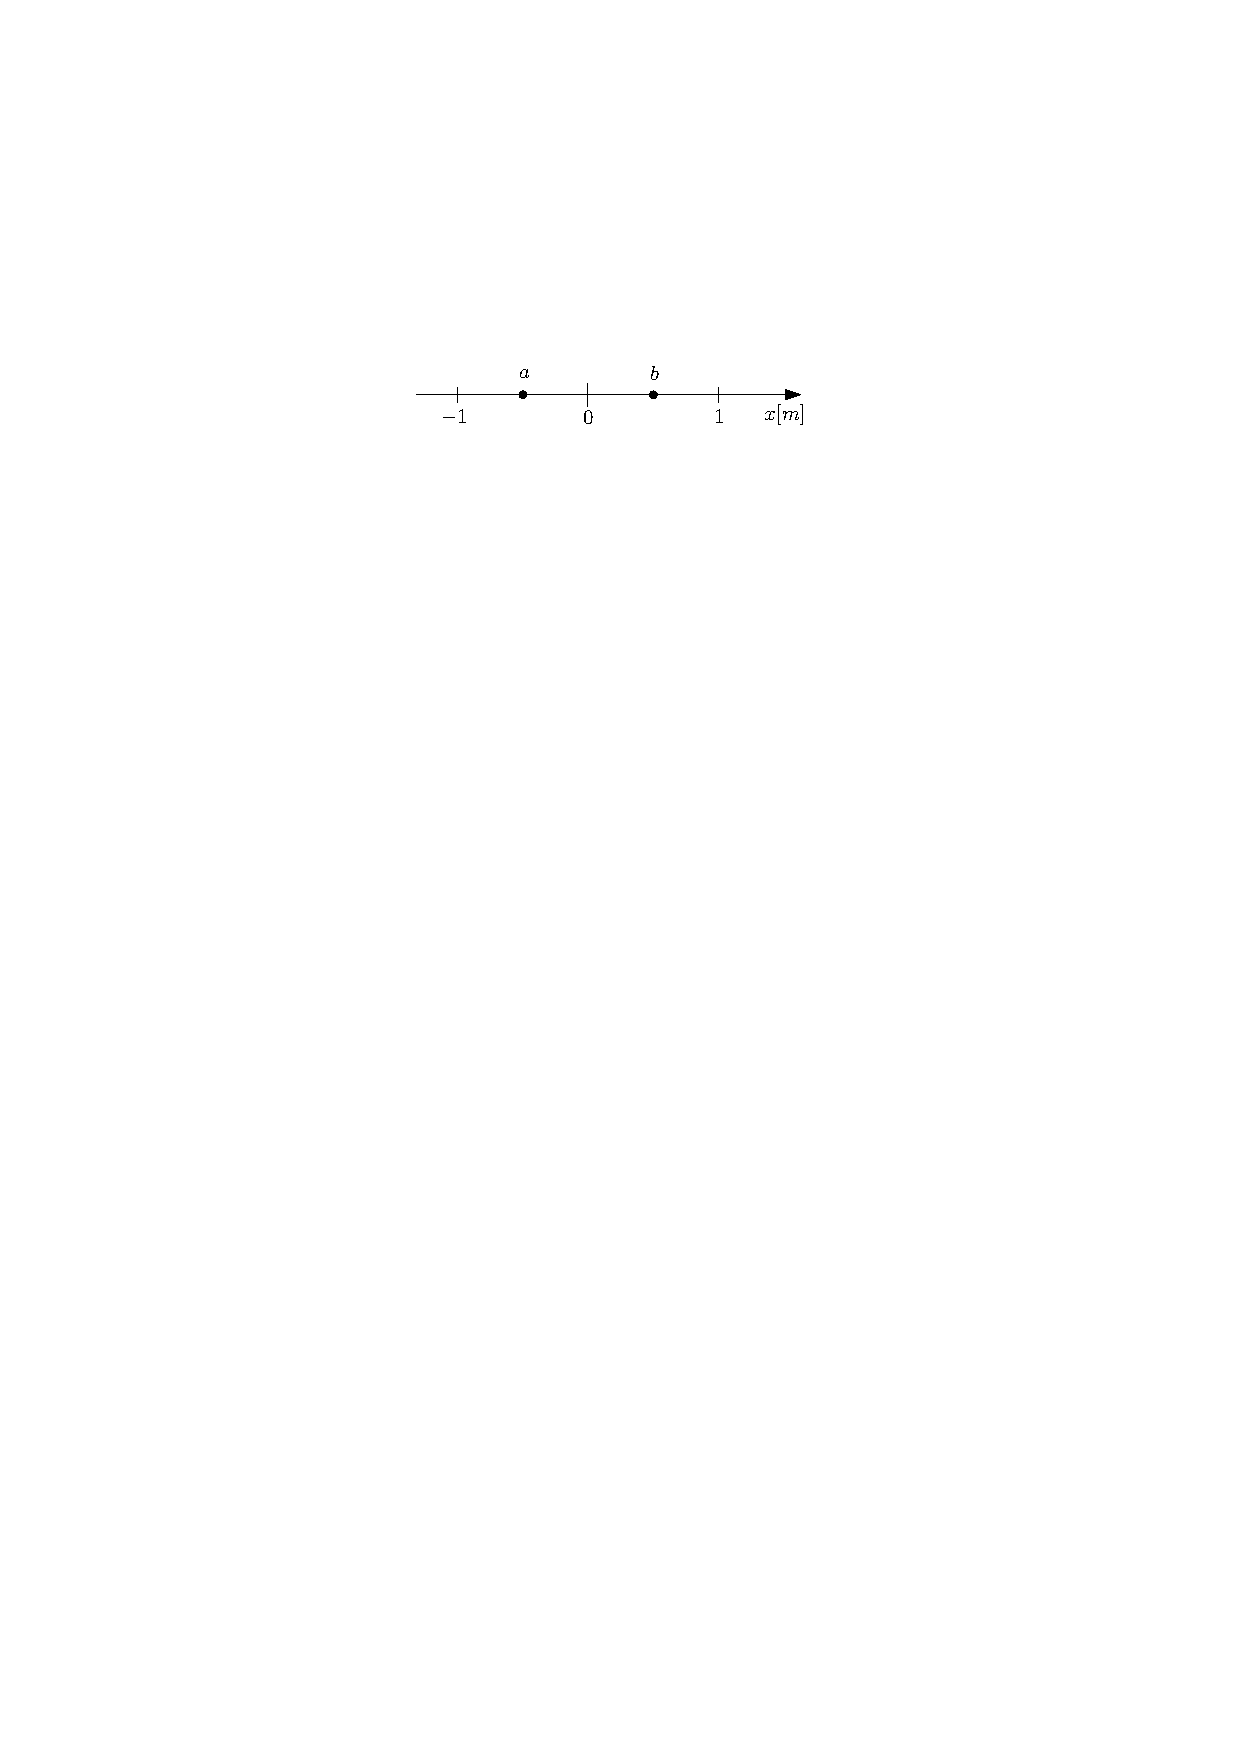
\includegraphics[width=.9\linewidth]{img/p_t_d_ej3.pdf}
	\caption{Una partícula se mueve desde $a$ hasta $b$ y luego de $b$ hacia $a$}	
\end{subfigure} 
 \begin{subfigure}{0.5\textwidth}
    \centering
 	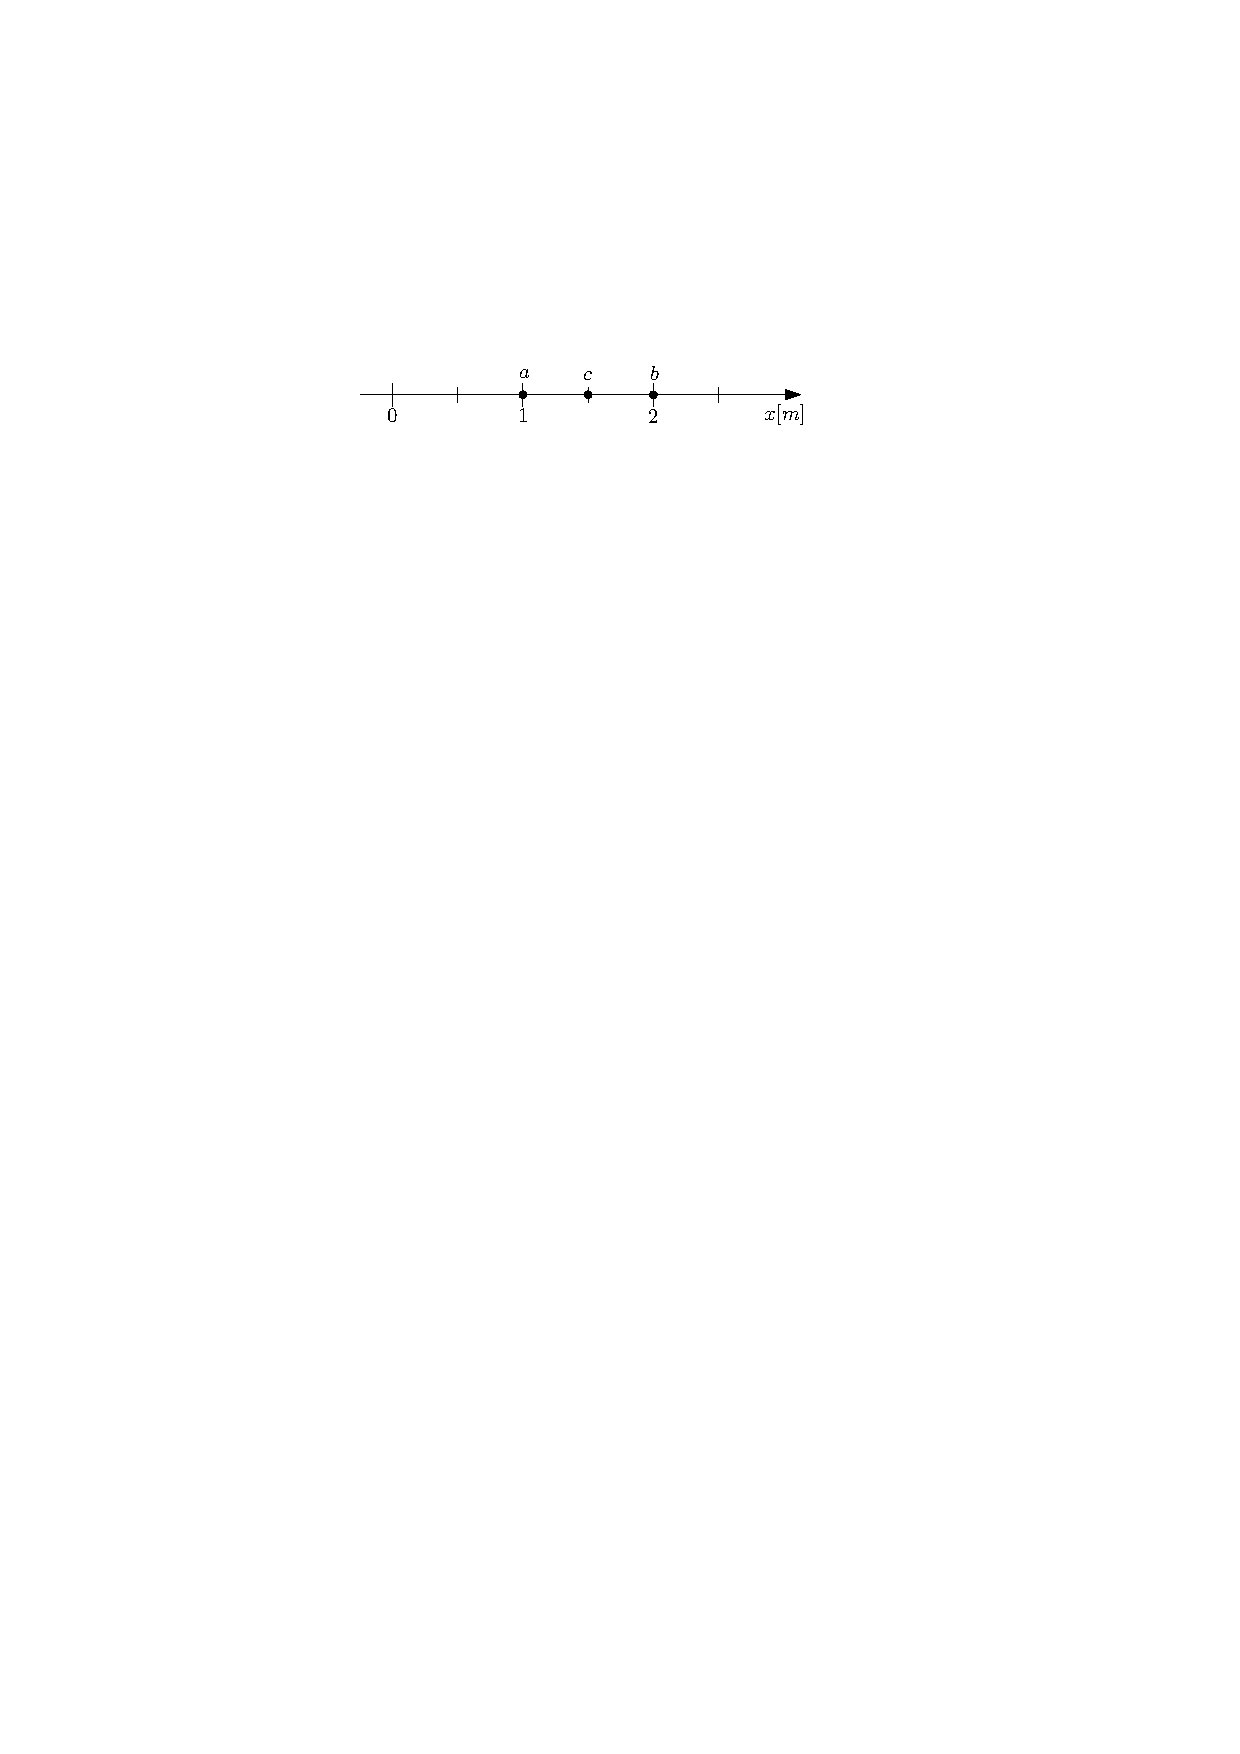
\includegraphics[width=.9\linewidth]{img/p_t_d_ej2.pdf}
	\caption{Una partícula se mueve desde $a$ hasta $b$ y finalmente hasta $c$.}	
\end{subfigure} 
\end{figure}

\noindent
{\bf Tercero:}

En base a lo que has pensado anteriormente, responde:
\begin{enumerate}
\item ¿Puede una partícula recorrer una distancia y que su desplazamiento sea nulo?
\item En una trayectoria rectilínea, ¿coincide siempre la distancia recorrida con el módulo del desplazamiento?
\end{enumerate}
\end{comprension}

\section{Velocidad}

\subsection{Velocidad media}

La \textbf{velocidad media }de una partícula se define como la razón entre su desplazamiento {$\mathbold{\bar{d}}$} y el intervalo de tiempo $\Delta t$ en que se produce dicho desplazamiento:

$$\mathbold{\bar{v}_m}\ = \ \frac{\mathbold{\bar{d}}}{\Delta t}$$

en donde dicha velocidad es una magnitud {\it vectorial} la cual tiene la misma dirección y sentido que el desplazamiento debido a que $\Delta t > 0$.


En el caso particular de un movimiento rectilíneo, la velocidad media queda de la forma:

\begin{center}
\boxed{\mathbold{\bar{v}_m} \ = \ \frac{\mathbold{\Delta \bar{x}}}{\Delta t}}
\end{center}

gráficamente:

\begin{figure}[h!]
\center
 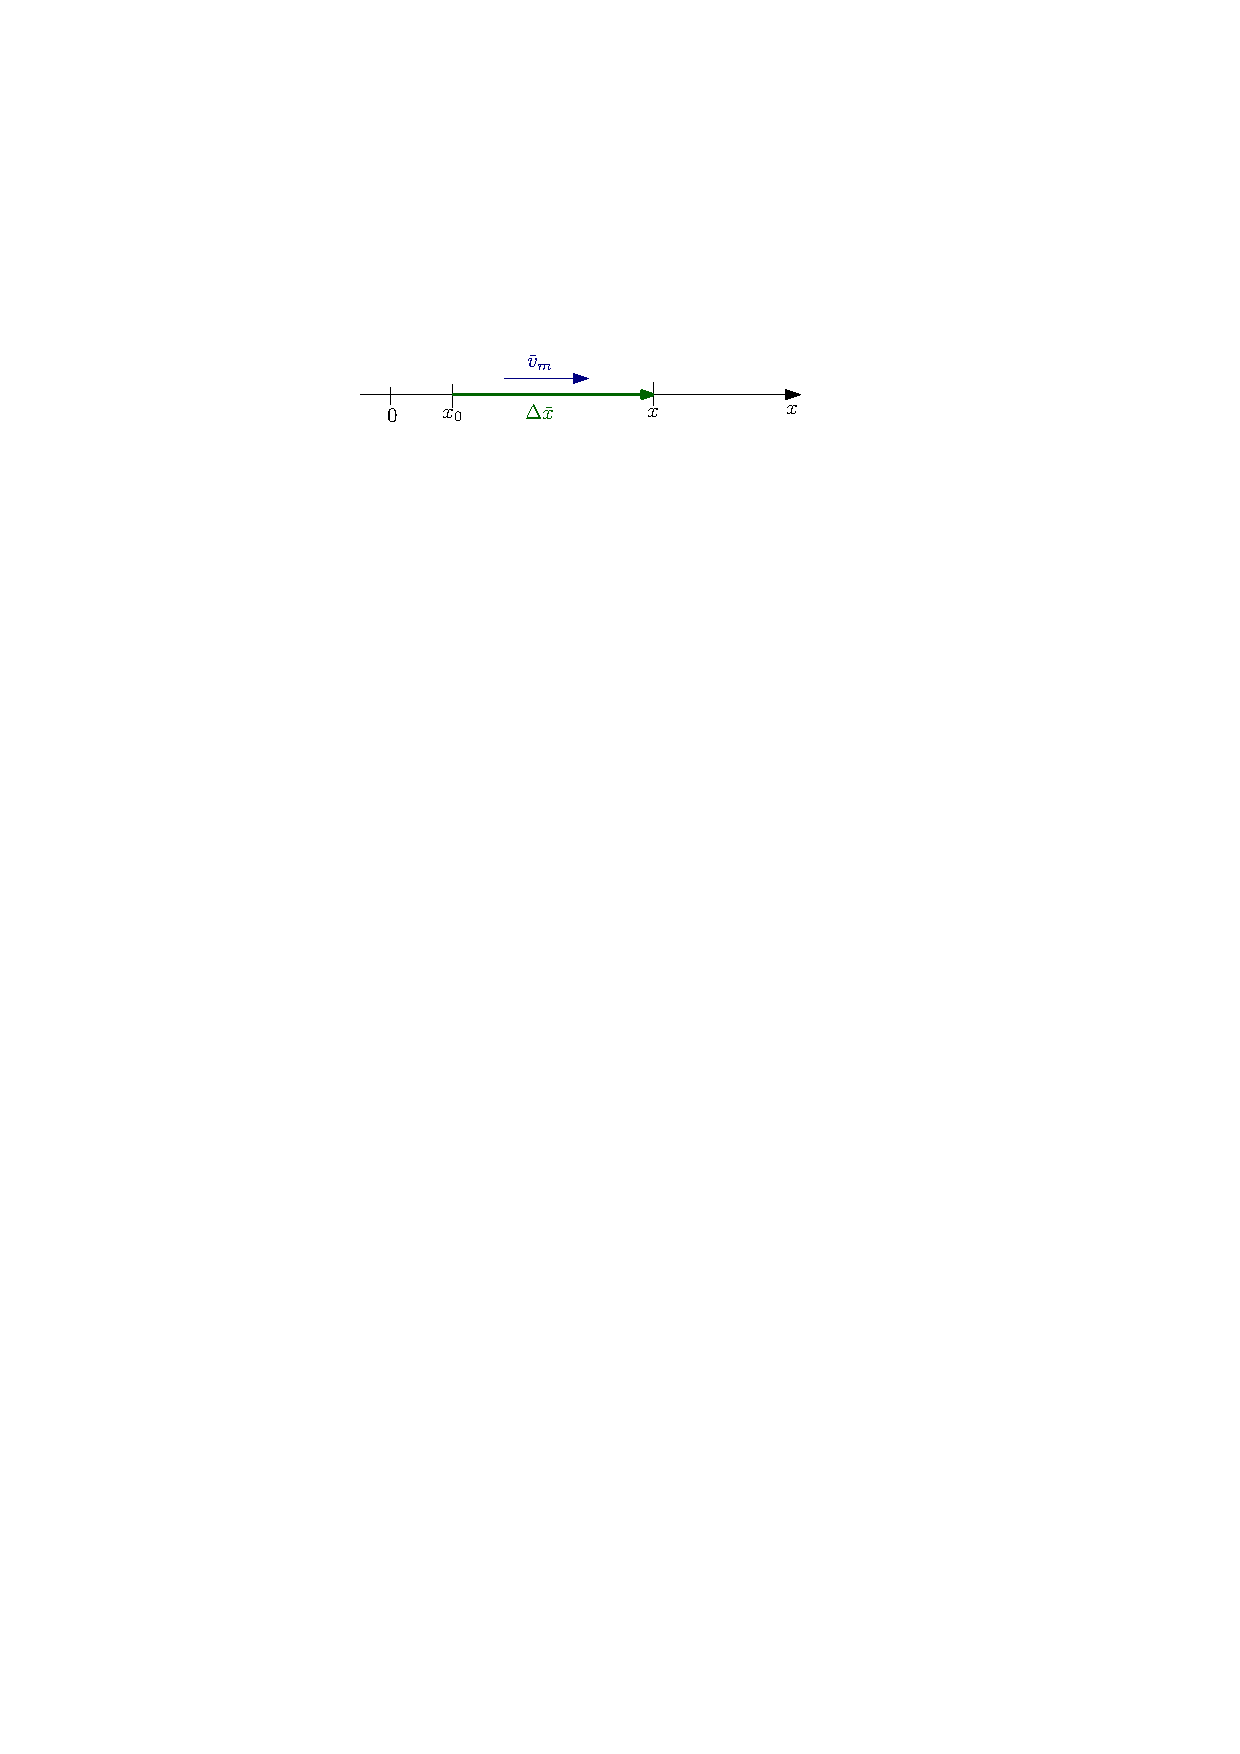
\includegraphics[width=.5\textwidth]{img/vm.pdf}
  \caption{Velocidad media en un movimiento rectilíneo.}
\end{figure}


Las unidades con que se miden las velocidades surgen de la misma operación que las define. Se trata de un cociente entre una longitud ($\Delta x$) y un intervalo de tiempo ($\Delta t$). Con esta expresión: $$[v_m] = \frac{[\Delta x]}{[\Delta t]}$$
Si trabajamos en el SIMELA, la unidad derivada es:$$[v_m] = \sif{m}{s}$$

\begin{comprension}

  \noindent{\bf Primero:}

Supongamos que un automóvil está viajando hacia Rosario. ¿Que le preguntarías al conductor para determinar la \textit{velocidad media} de su movimiento?

\noindent
{\bf Segundo:}

Un automóvil se desplaza desde Rosario hasta Buenos Aires como muestra la figura. Dicho móvil tarda 3 horas en llegar a destino. Determina la velocidad media del automóvil entre las ciudades de Rosario y Buenos Aires.


\begin{figure}[H]
\centering
 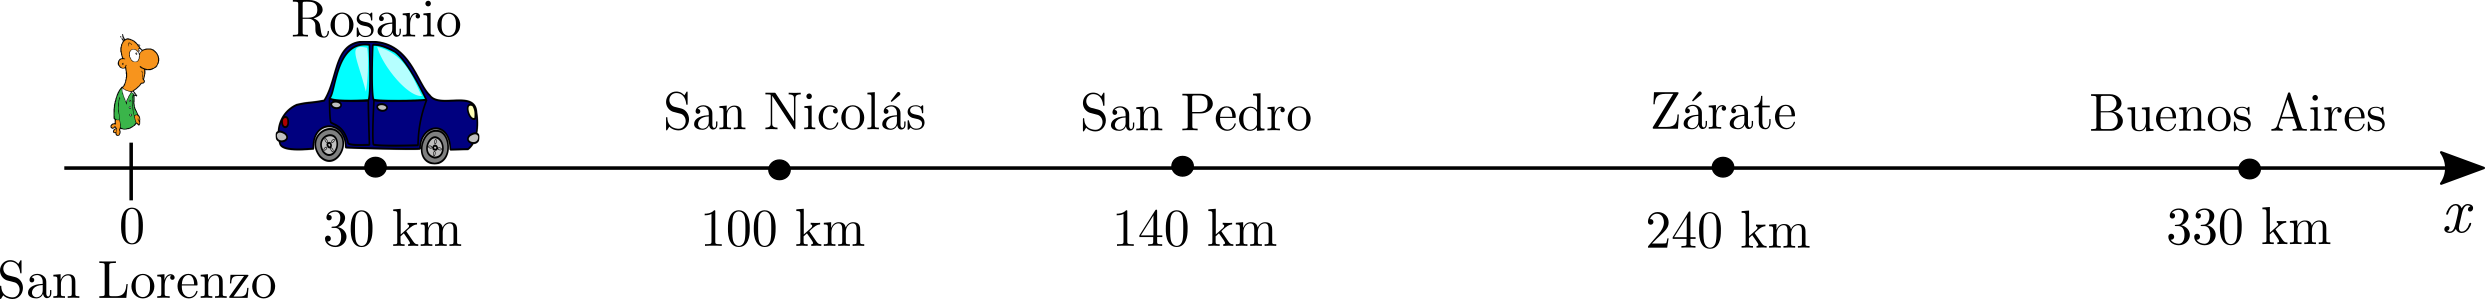
\includegraphics[width=.9\textwidth]{img/viaje.png}
 % \caption{Velocidad media en un movimiento rectilíneo.}
\end{figure}

Para ayudarte, representa gráficamente las posiciones inicial y final, el desplazamiento y luego la velocidad media:

\begin{figure}[H]
\centering
 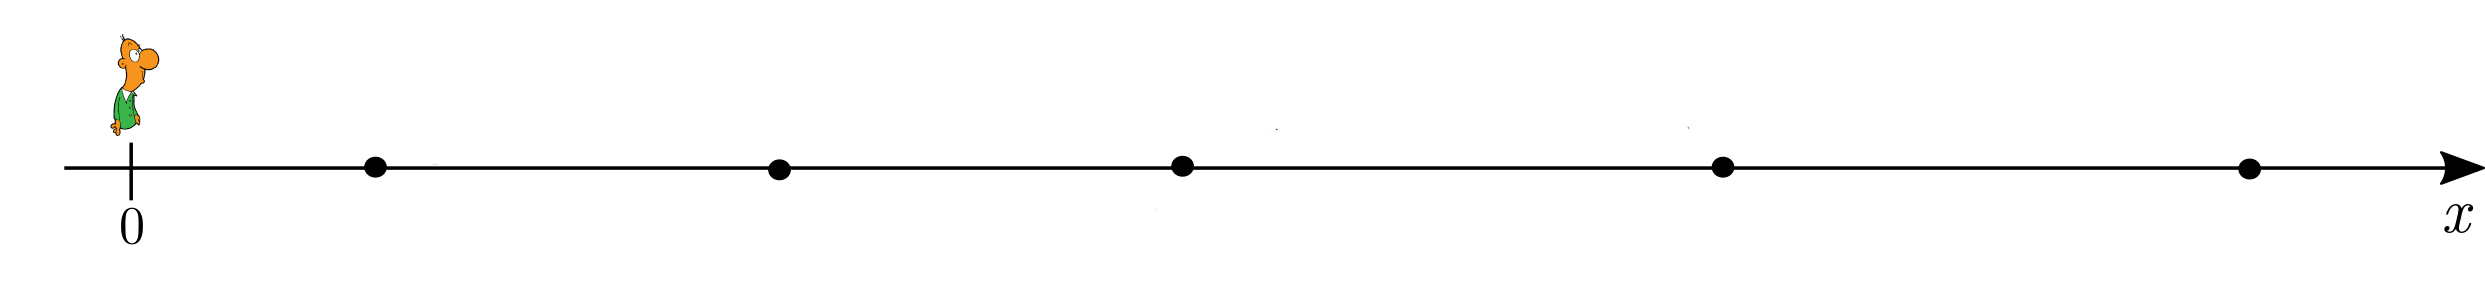
\includegraphics[width=.9\textwidth]{img/viaje2.png}
 % \caption{Velocidad media en un movimiento rectilíneo.}
\end{figure}



A partir de la información de la velocidad media conseguida. ¿Podemos saber cuál era la velocidad del automóvil cuando pasaba por San Nicolás? ¿Y por Zárate? ¿Podemos saber si se detuvo a descansar en San Pedro?
\end{comprension}

\subsection{Velocidad Instantánea}

\info{
    Antes de definir {\it velocidad instantánea} debemos destacar que la palabra {\bf instante} tiene un significado un poco distinto en física que en el lenguaje cotidiano. Podemos utilizar la frase ``duró sólo un instante'' para referirnos a algo que duró un intervalo de tiempo muy corto. Sin embargo, en física un instante no tiene duración; es un solo valor de tiempo.}

Podemos definir la {\bf velocidad instantánea} como la velocidad de una partícula en cualquier {\it instante} de tiempo.

Supongamos que una partícula viaja desde {$\mathbold{P_0}$} hasta {$\mathbold{P}$} por la trayectoria {$\mathbold{T}$}, definiendo un desplazamiento {$\mathbold{\bar{d}}$}:

La velocidad media de este movimiento podríamos determinarla: $\mathbold{\bar{v}_m}=\frac{\mathbold{\bar{d}}}{\Delta t}$

\begin{figure}[!h]
\centering
 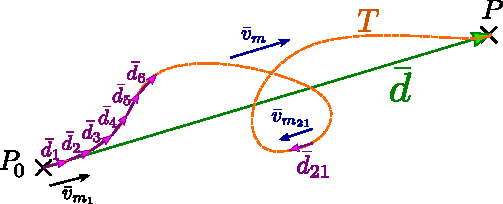
\includegraphics[width=.6\textwidth]{img/velocidad_instantanea.pdf}
 \caption{\label{fig:particion_tray} Una trayectoria cualquiera se puede dividir en pequeños intervalos. En cada intervalo, el desplazamiento se parecerá mucho más a la trayectoria.}
\end{figure}


Si dividimos la trayectoria total en pequeñas trayectorias, como muestra la Figura~\ref{fig:particion_tray}, podríamos definir pequeños intervalos de desplazamiento ({$\mathbold{\bar{d}_1; \bar{d}_2;...}$}). Observemos que cada uno de estos desplazamientos ocurren en ciertos intervalos de tiempo ({$\Delta t_1; \Delta t_2;...$}). Así, podremos calcular también distintas velocidades medias para cada uno de estos intervalos. 

Tomemos, como ejemplo, que el desplazamiento {$\mathbold{\bar{d}_{21}}$} ocurre en el intervalo de tiempo {$\Delta t_{21}$} por lo tanto, la partícula, en ese intervalo, tendría una velocidad media dada por: $$\mathbold{\bar{v}_{m_{21}}} = \frac{\mathbold{\bar{d}_{21}}}{\Delta t_{21}}$$

Vemos que la velocidad $\mathbold{\bar{v}_{m_{21}}}$ describe mucho mejor el comportamiento de la partícula en ese tramo de trayectoria que la velocidad $\mathbold{\bar{v}_m}$.

Si tomamos intervalos de tiempo cada vez más chicos, veremos que los valores de velocidad media se acercan a los de velocidad instantánea. ¡Y así podremos saber cuál es la velocidad del automóvil en el instante en que pasa por San Pedro!

Podemos decir que a medida que el intervalo de tiempo {\em tiende a cero} o se aproxima lo suficientemente a cero,  la velocidad media tiende a la velocidad instantánea, en cada intervalo considerado. El concepto matemático de aproximación a un valor pero sin llegar al mismo se denomina {\bf \em límite}. La definición rigurosa de {\bf \em velocidad instantánea} usa dicho concepto:
$$\mathbold{\bar{v}_{m_{21}}} = \lim_{\Delta t \rightarrow 0} \mathbold{\bar{v}_m} = \lim_{\Delta t \rightarrow 0}\frac{\mathbold{\bar{d}}}{\Delta t}$$
Sin embargo, en nuestro caso, lo importante no es usar esta definición matemáticamente rigurosa, sino comprender conceptualmente lo que acabamos de analizar.

En el caso particular de un movimiento rectilíneo, la velocidad instantánea queda de la forma:
$$\mathbold{\bar{v}} = \lim_{\Delta t \rightarrow 0} \mathbold{\bar{v}_m} = \lim_{\Delta t \rightarrow 0} \frac{\mathbold{\Delta \bar{x}}}{\Delta t}$$


La velocidad es una magnitud vectorial. Pensemos en dos automóviles que se mueven por la misma ruta en sentidos opuestos a 60 km/h y 70 km/h respectivamente. Refiriendo estas velocidades al sistema de coordenadas resultarán de signos opuestos:

%% Acá hay que ponerse de acuerdo en cómo vamos a decir lo del signo.

\begin{figure}[h!]
\centering
 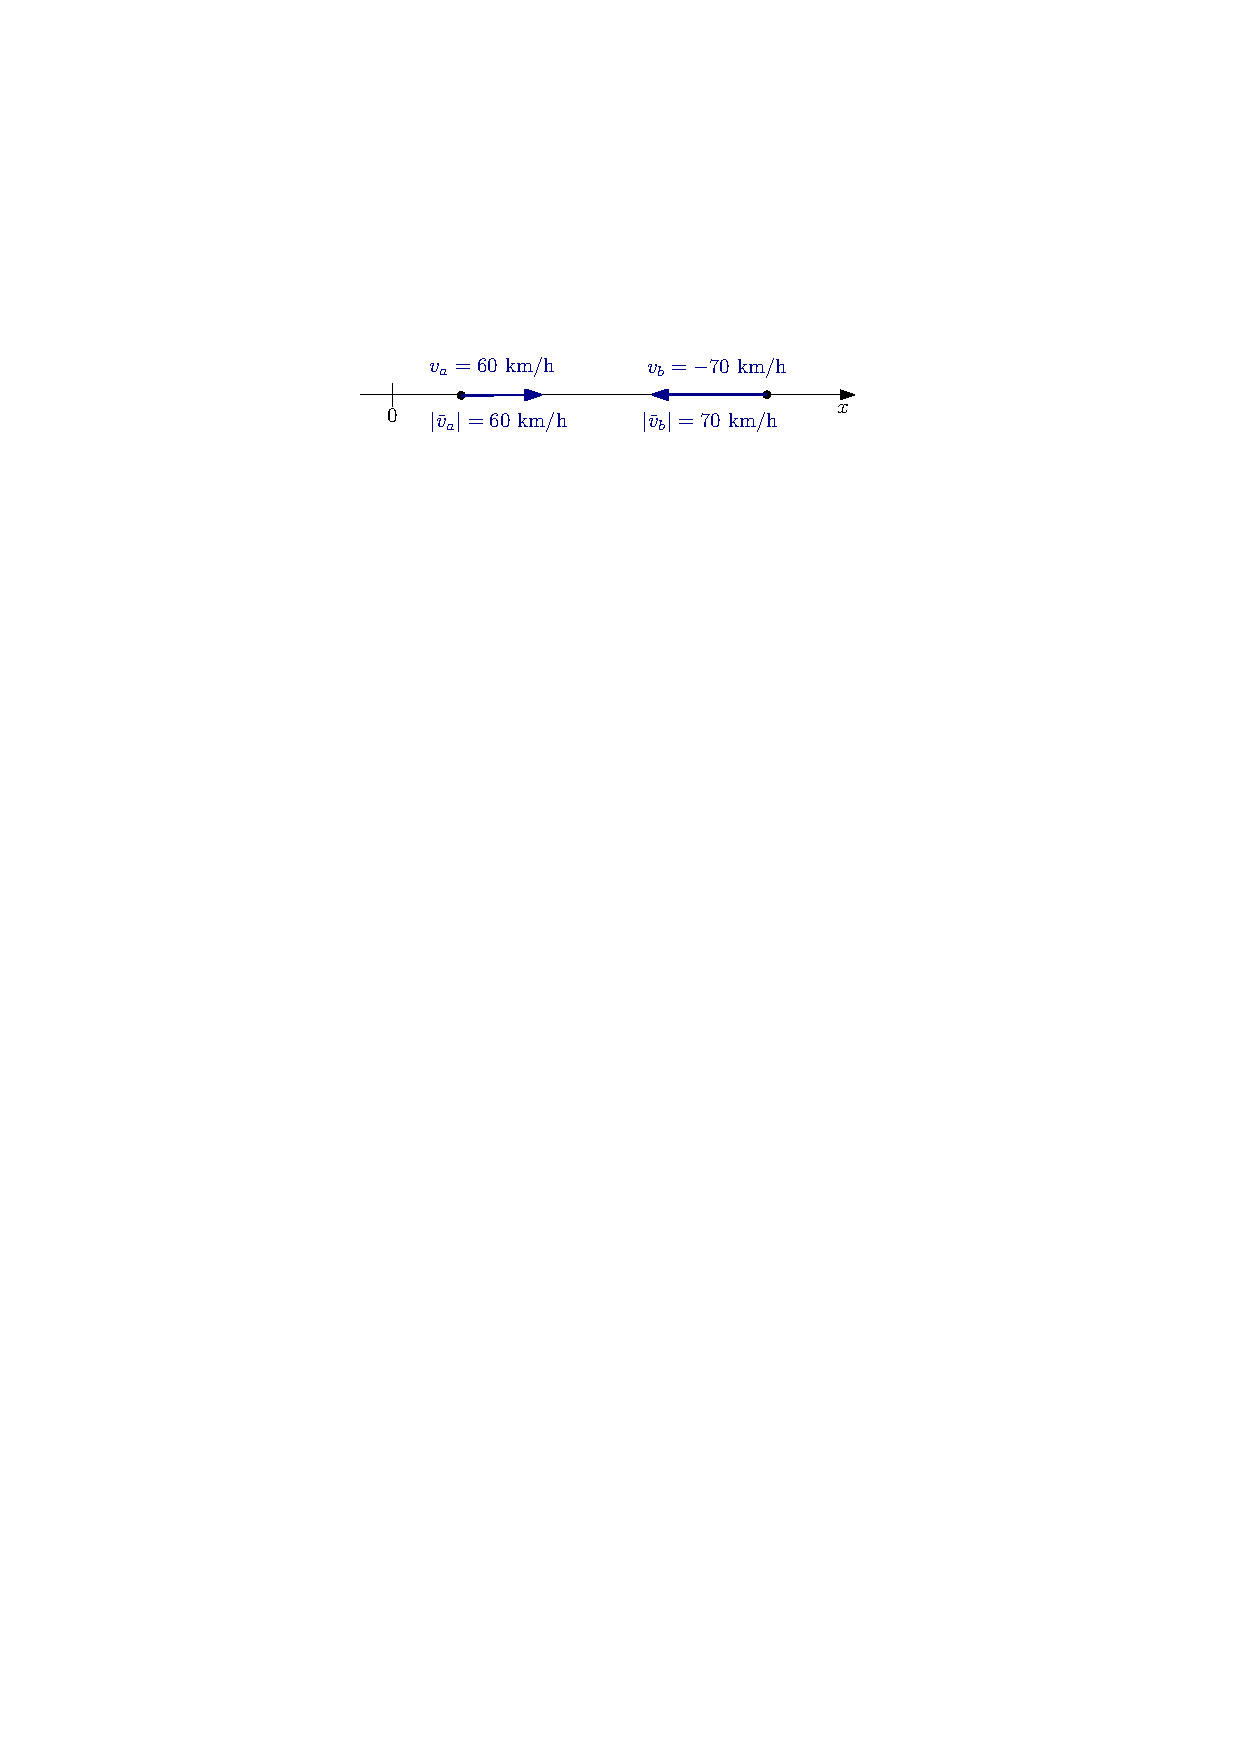
\includegraphics[width=.6\textwidth]{img/velocidad_instantanea2.pdf}
 % \caption{Velocidad media en un movimiento rectilíneo.}
\end{figure}
El signo de la velocidad \textbf{depende del sistema de coordenadas} y nos indica el sentido del movimiento.


{\bf \color{BrickRed} {¡Cuidado!}} En el ejemplo anterior, cuando decimos ``$v_a= 60$ km/h'' o ``$v_b= -70$ km/h'', {\bf ¡nos estamos refiriendo a la componente $\mathbold{x}$ del vector velocidad!} Debido a que el movimiento es rectilíneo, es decir que la partícula se mueve en el eje $x$, podemos utilizar esta notación. Si el movimiento fuera en un plano deberíamos escribir sus dos componentes:

\begin{figure}[h!]
\centering
 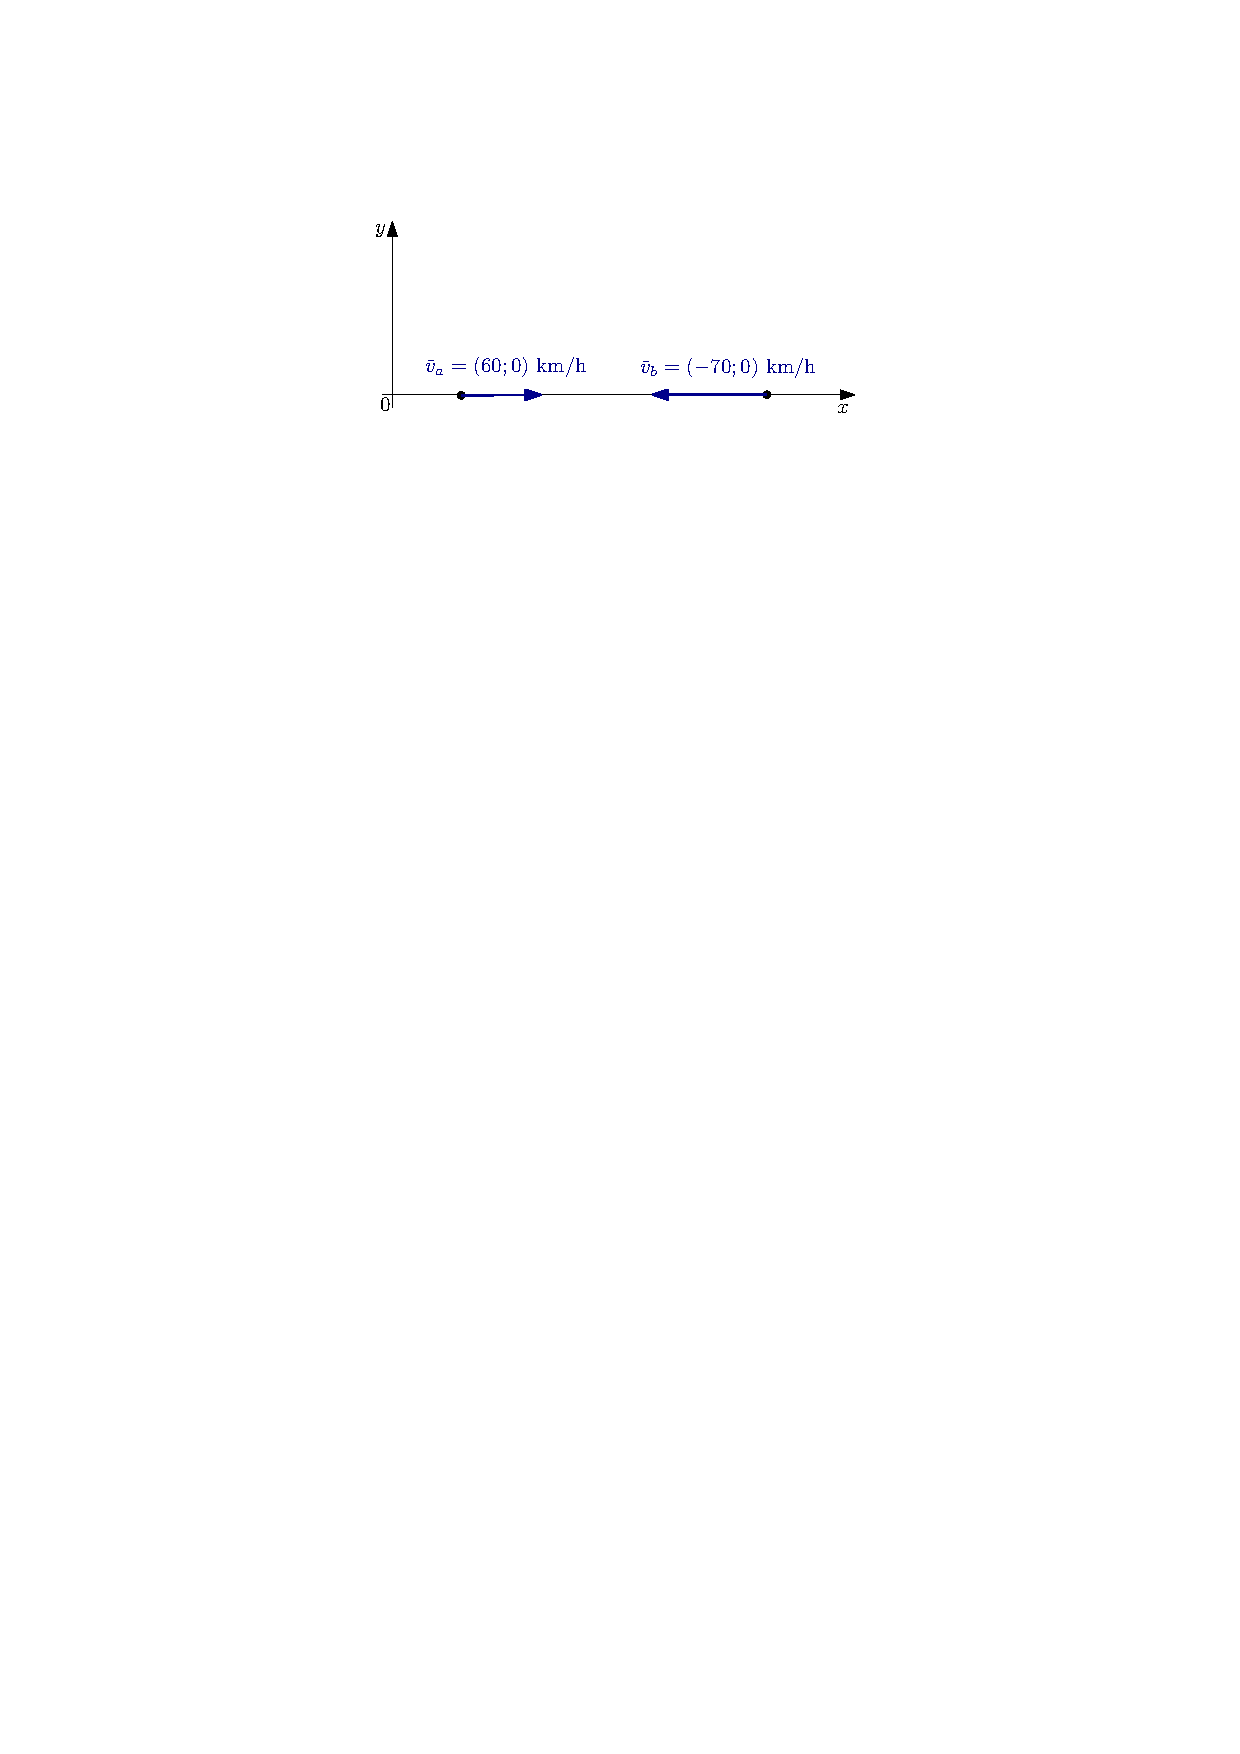
\includegraphics[width=.6\textwidth]{img/velocidad_instantanea3.pdf}
 % \caption{Velocidad media en un movimiento rectilíneo.}
\end{figure}

La \textbf{rapidez} de una partícula se define como el {\bf ``módulo''} de su velocidad. La rapidez no tiene dirección asociada y, en consecuencia, no lleva signo algebraico. Por ejemplo si una partícula tiene una velocidad de +25 m/s y otra de –25 m/s sobre el eje $x$, las dos tienen una rapidez de 25 m/s. El velocímetro de un automóvil indica la rapidez instantánea y no la velocidad instantánea.



%%%%%%%%%%%%%%%%%%
% \end{document}
 

%% Acá va la sección de MRU
\section{Movimiento Rectilíneo Uniforme}

Podríamos decir que uno de los objetivos principales de la mecánica es poder realizar predicciones sobre el movimiento de una partícula, conocido su estado inicial de movimiento.

Ahora bien, de acuerdo con lo estudiado en la sección anterior, uno podría imaginar que la velocidad instantánea de una partícula varía de cualquier forma a medida que transcurre el tiempo. De esta manera, realizar predicciones del comportamiento de la partícula, se volvería una tarea súmamente complicada. En vistas de ello, nos restringiremos en este capítulo a los movimientos más simples: el Movimiento Rectilíneo Uniforme y el Uniformemente Variado. Comenzaremos por el primero y, luego de aprender el concepto de aceleración, veremos el segundo tipo de movimiento.

Uno podría pensar que se está perdiendo de mucha información si se limita a estudiar el movimiento rectilíneo. Pues bien, en los próximos capítulos veremos que, en muchas situaciones cotidianas, basta con estos dos tipos de movimiento para describir el comportamiento de los cuerpos, y que combinando estos dos se pueden describir movimientos más complejos como el tiro parabólico.

El {\bf Movimiento Rectilíneo Uniforme (MRU) es un movimiento con rapidez constante en una trayectoria rectilínea}. Decir que la trayectoria es rectilínea significa decir que el vector velocidad instantánea se mantiene sobre una recta determinada. Que el movimiento sea uniforme implica que la rapidez es constante. Que la rapidez sea constante significa que el módulo de la velocidad permanece invariable a lo largo del tiempo. Dado que no existe en la naturaleza ningún cuerpo capaz de cambiar el sentido de su vector velocidad sin antes detenerse\footnote{Más adelante estudiaremos el caso de partículas que cambian el sentido de su movimiento muy rápidamente y veremos que siempre existe un pequeño intervalo de tiempo, muy corto para que nosotros lo percibamos, en el que la partícula cambia el sentido de su movimiento.}, esto también significa que la velocidad siempre apuntará en el mismo sentido. Como, al mismo tiempo, la dirección, el módulo y el sentido del vector velocidad permanecen constantes, podemos decir que la velocidad instantánea es un vector constante. Lo expuesto hasta aquí se puede resumir en un mapa conceptual:

\begin{figure}[!h]
  \centering
  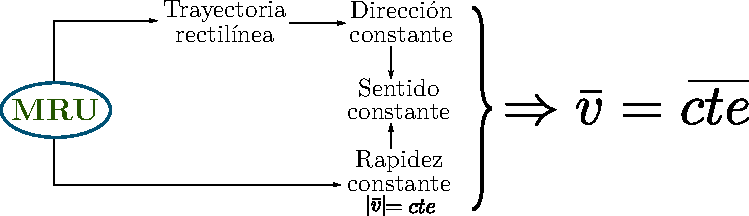
\includegraphics[scale=1]{img/cuadro_MRU.pdf}
\end{figure}

Dado que la velocidad es constante, en todo momento esta será igual a la velocidad media, por lo que
$$\mathbold{\bar{v}}=\mathbold{\bar{v}_m}=\frac{\mathbold{\Delta \bar{x}}}{\Delta t}$$
De esta manera, también se cumple que $\mathbold{\bar{v}} \Delta t=\mathbold{\Delta\bar{x}}$.

Dado que solo tenemos una dimensión, podemos hacer los cálculos directamente utilizando las componentes de los vectores involucrados. Así, podemos escribir:
$${v}(t-t_0)={x}-{x}_0$$
Si despejamos ${x}$ en la ecuación anterior obtenemos
$${x}={x}_0+{v}(t-t_0)$$
o bien
\begin{center}
{\color{NavyBlue}  \boxed{\mathbold{{x}={x}_0+{v}\Delta t}}}
\end{center}

La ecuación anterior se conoce como {\em ``Ley de movimiento del MRU''} o {\em ``Ley horaria''}, y nos permite determinar la posición de una partícula en cada instante de tiempo, conocida su velocidad y su posición inicial.

En muchas situaciones de interés, esta ecuación se puede simplificar tomando $t_0=0$, y así nos queda $${x}={x}_0+{v}t$$
Vamos a ver cómo se utiliza la ley de movimiento en una situación práctica:

\begin{example}{Ejemplo:}
  {\it Un juego muy popular antes del advenimiento de Internet era ``la bolita''. Un tiempo después de haber sido disparada, una bolita de vidrio se encuentra a 20 cm de una pared y se mueve con una rapidez constante de 0,5 m/s alejándose de la misma. Determina a qué distancia se encontrará de la pared al cabo de 2 s, 4 s, 6 s, y 8 s.}
  \tcblower
  {\sf {\bf Modelo:} Supondremos en este problema que la bolita es una partícula que se mueve en una trayectoria rectilínea con rapidez constante.}
  
El primer paso para resolver un problema de física es realizar un esquema de la situación física identificando los datos del problema:
  \begin{center}
    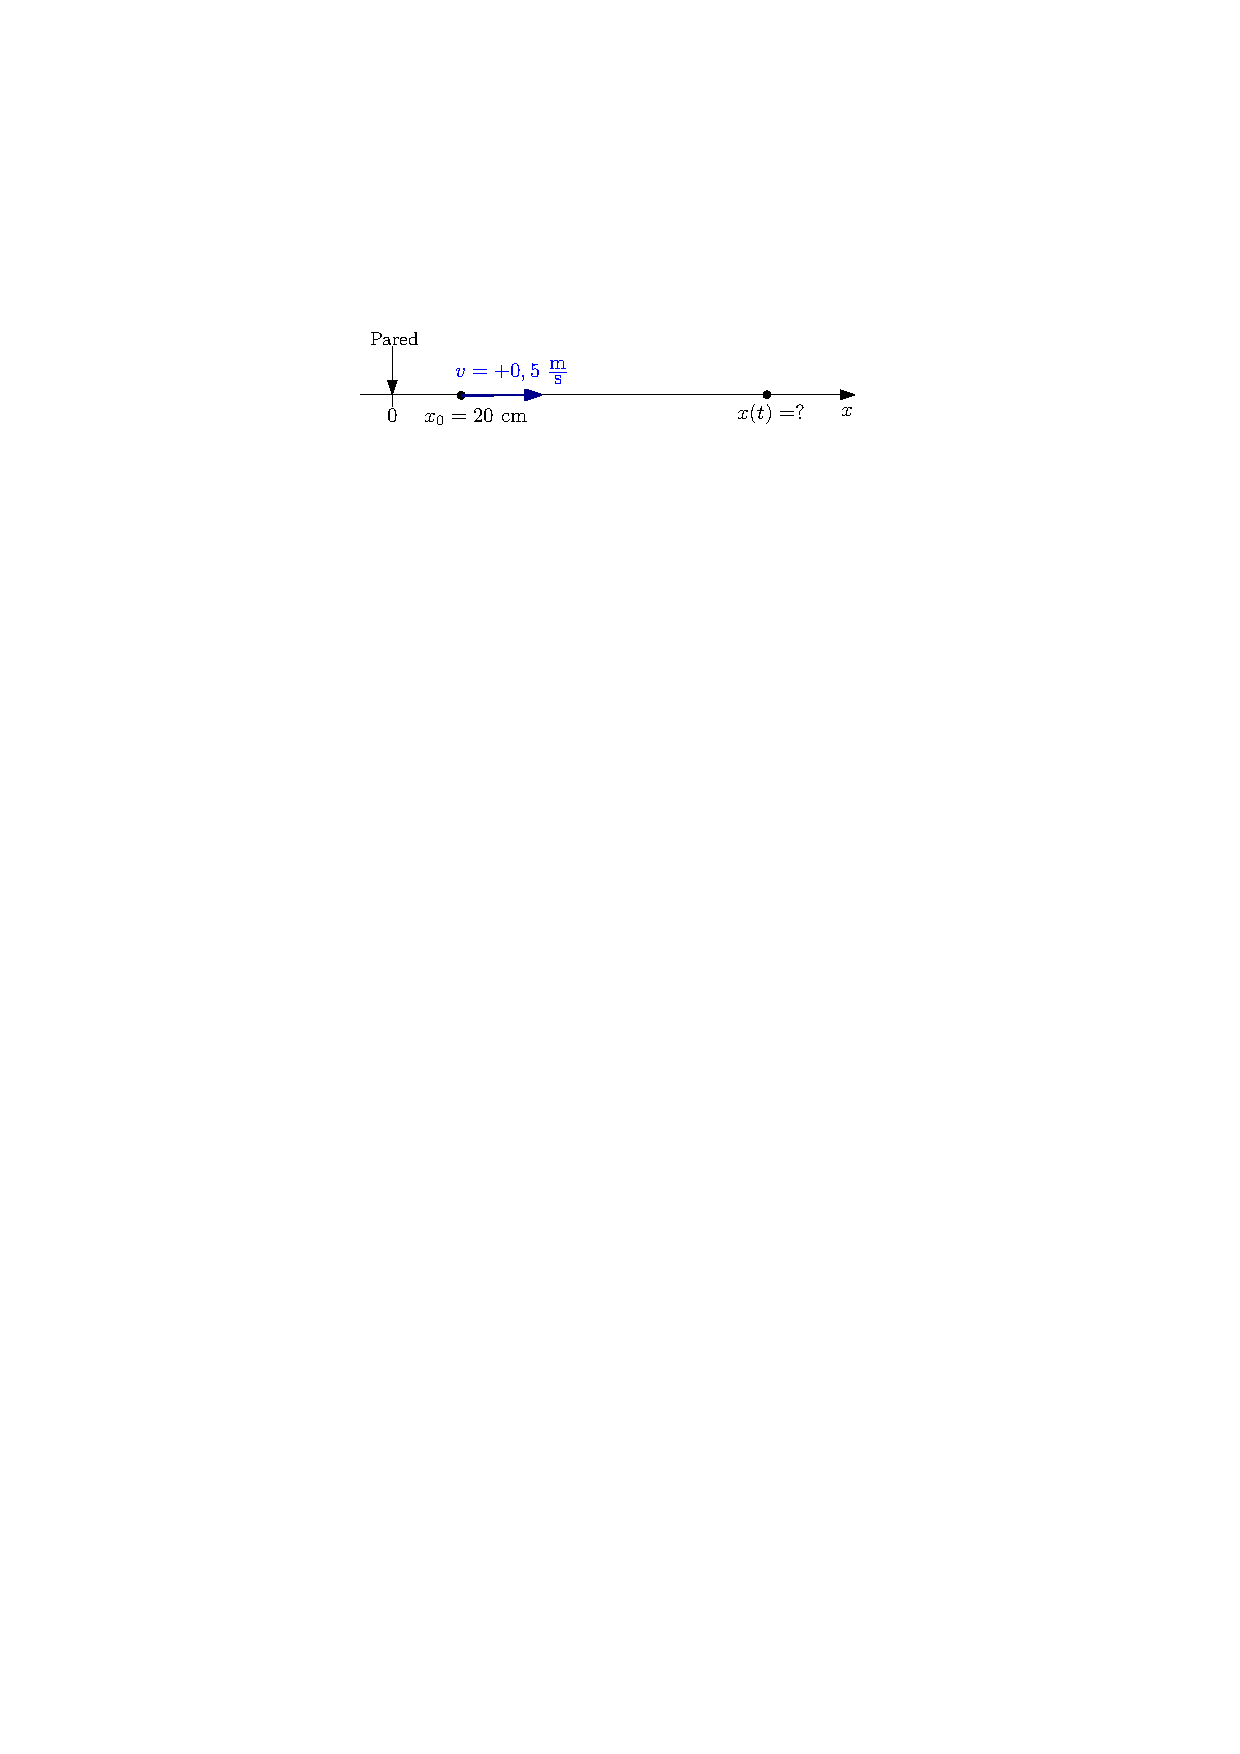
\includegraphics[]{img/bolita.pdf}
  \end{center}
  Dado que hemos colocado el origen de coordenadas de nuestro sistema de referencia en la pared, determinar la distancia de la bolita a la pared significa determinar la posición de la bolita en {\em nuestro} sistema de referencia.
  Debemos procurar que todos los datos estén en el mismo sistema de unidades. En nuestro caso, la posición inicial de la bolita está en un submúltiplo del metro, así que la expresamos en metros: $x_0=0.20$~m. Tomaremos para este problema, $t_0=0\si{s}$.

  Ahora que ya tenemos todos los datos, podemos utilizarlos para calcular la posición de la bolita respecto de la pared en los instantes pedidos:
  $$2\si{s}:\quad x = x_0 + vt = 0.20\si{m} + 0,5\sif{m}{s} \cdot 2\si{s} = 1.20\si{m}$$
  $$4\si{s}:\quad x = x_0 + vt = 0.20\si{m} + 0,5\sif{m}{s} \cdot 4\si{s} = 2.20\si{m}$$
  $$6\si{s}:\quad x = x_0 + vt = 0.20\si{m} + 0,5\sif{m}{s} \cdot 6\si{s} = 3.20\si{m}$$
  $$8\si{s}:\quad x = x_0 + vt = 0.20\si{m} + 0,5\sif{m}{s} \cdot 8\si{s} = 4.20\si{m}$$
\end{example}

La información del Ejemplo anterior se puede volcar en una gráfica en la que representemos la posición de la bolita a medida que transcurre el tiempo. Para realizar este tipo de gráficas, decimos que {\bf la posición es función del tiempo} y lo notamos $\mathbold{x=x(t)}$. La gráfica en cuestión se muestra en la Figura~\ref{fig:grafica_MRU_x}.


\begin{figure}[!h]
  \centering
  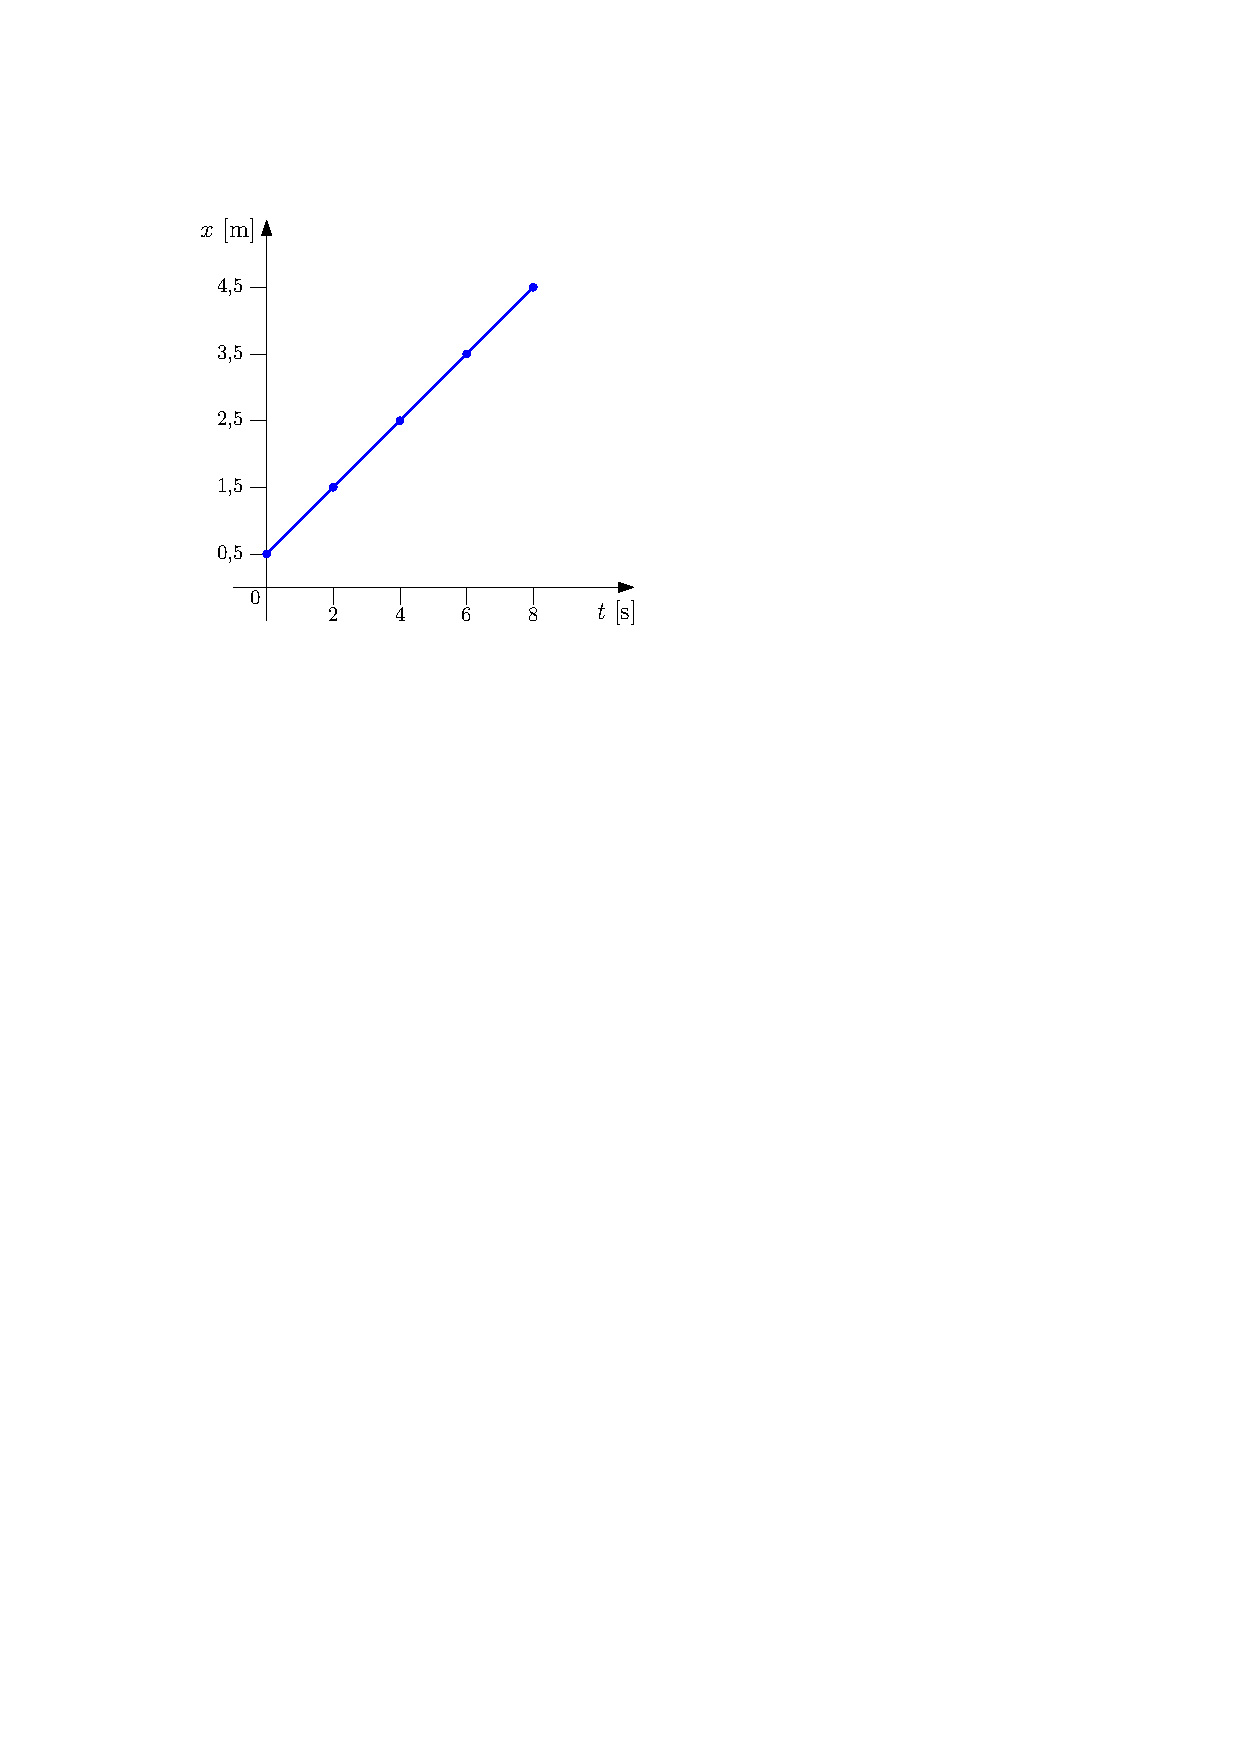
\includegraphics[scale=1]{img/grafica_MRU_x.pdf}
  \caption{\label{fig:grafica_MRU_x} Gráfica típica $x=x(t)$ de un MRU.}
\end{figure}

¿Qué podemos decir de esta gráfica? Lo primero que podemos ver, es que los puntos que se obtienen al graficar están alineados sobre una misma recta. Esto también pasará para cualquier otro instante de tiempo en este mismo movimiento. ¿Por qué? Porque al ser la rapidez constante, {\em en tiempos iguales nuestra bolita recorrerá distancias iguales}. Esta es una de las principales características del Movimiento Rectilíneo Uniforme: La gráfica $x=x(t)$ siempre será una recta.

Otra cosa que observamos de la gráfica, es que la recta corta al eje de las ordenadas en un valor que es ni más ni menos que la posición inicial $x_0$ de la partícula.

También vemos que, a medida que transcurre el tiempo, la posición va tomando valores positivos cada vez mayores. Esto es consistente con el enunciado del problema y con el sistema de referencia elegido: {\em A medida que transcurre el tiempo, la bolita se va alejando del origen de coordenadas, situado en la pared, en el sentido elegido como positivo para el sistema de referencia.}

Grafiquemos ahora la velocidad de nuestra partícula a medida que trancurre el tiempo. Nuestra tarea ahora es mucho más sencilla, puesto que el módulo y el sentido de la velocidad se mantienen constantes a lo largo del tiempo. La gráfica $v=v(t)$ es, entonces, una recta horizontal, como lo muestra la Figura~\ref{fig:grafica_MRU_v}.

\begin{figure}[!h]
  \centering
  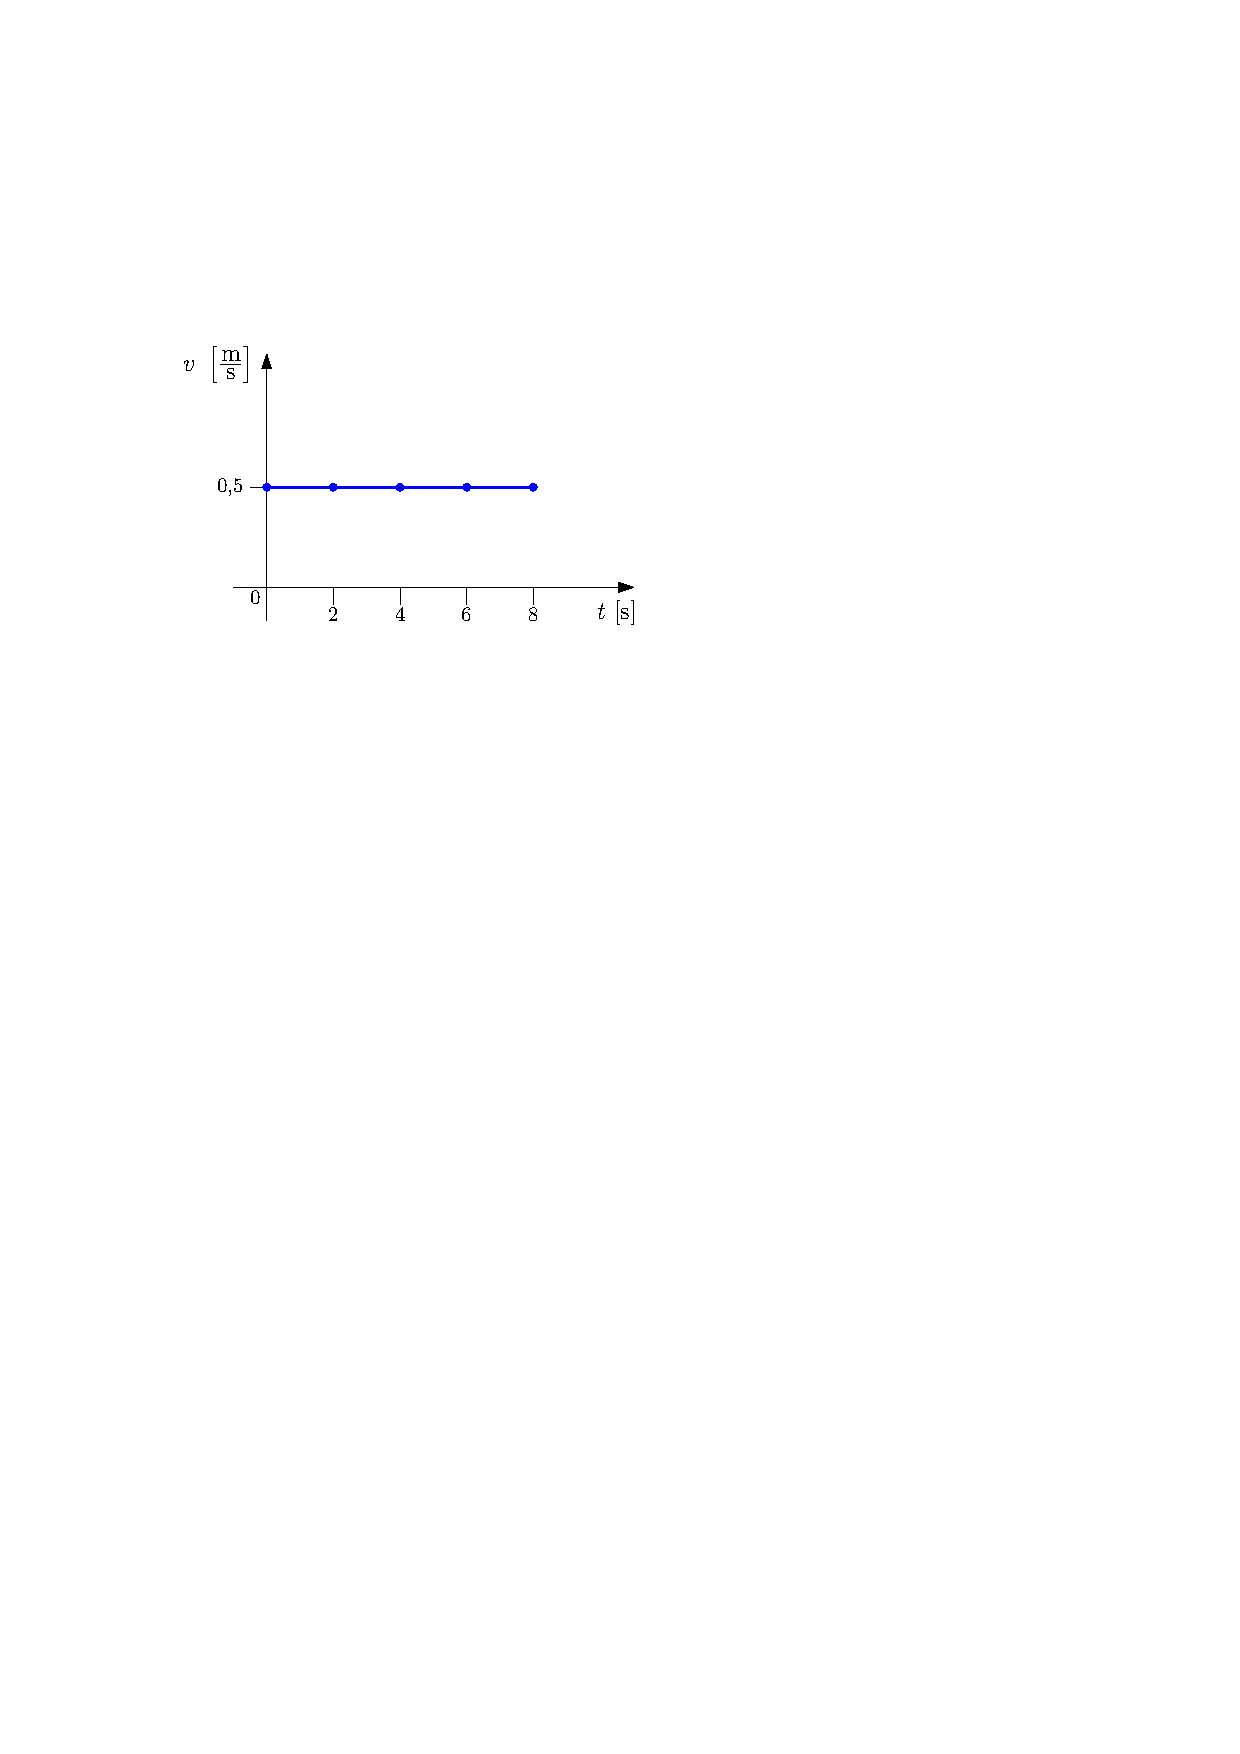
\includegraphics[scale=1]{img/grafica_MRU_v.pdf}
  \caption{\label{fig:grafica_MRU_v} Gráfica típica $v=v(t)$ de un MRU.}
\end{figure}

De esta gráfica podemos decir que la bolita tiene rapidez constante, y que el signo de la velocidad es positivo. Como el signo de la velocidad nos indica el sentido en el que la partícula se está moviendo, podemos decir que nuestra partícula se mueve en el sentido elegido como positivo, lo que es, nuevamente, consistente con el enunciado del problema, con el sistema de referencia que escogimos y, ahora también, con la gráfica $x=x(t)$ que analizamos anteriormente.

\info{Luego de realizar la gráfica de un movimiento cualquiera, uno siempre debe analizarla para corroborar que es consistente con el problema que acaba de resolver. Analizar una gráfica significa extraer de ella toda la información posible. Así, viendo las Figuras~\ref{fig:grafica_MRU_x} y \ref{fig:grafica_MRU_v}, deberíamos poder extraer la siguiente información: {\em Las gráficas muestran un móvil que originalmente se encuentra a $+0.5\si{m}$ del origen de coordenadas y, a medida que transcurre el tiempo, se va alejando del mismo, moviéndose en el sentido elegido como positivo para el sistema de referencia, con rapidez constante.}}

%%%%%%%%%%%%%%%%%%%%%%%%%%%%%%%%%%%%%%%%%%%%%%%
%   Cuadrito que habla sobre la pendiente     %
%%%%%%%%%%%%%%%%%%%%%%%%%%%%%%%%%%%%%%%%%%%%%%%
\begin{mybox}{Para profundizar}
  Si en la gráfica $x=x(t)$ del MRU elegimos un intervalo de tiempo $\Delta t_1$ y buscamos el desplazamiento $\Delta x_1$ que le corresponde, nos queda determinado un triángulo rectángulo $\overset{\triangle}{abc}$. Si ahora elegimos otro intervalo $\Delta t_2$ y marcamos su desplazamiento correspondiente $\Delta x_2$, nos queda determinado otro triángulo rectángulo $\overset{\triangle}{a'b'c'}$.
 \begin{center}
    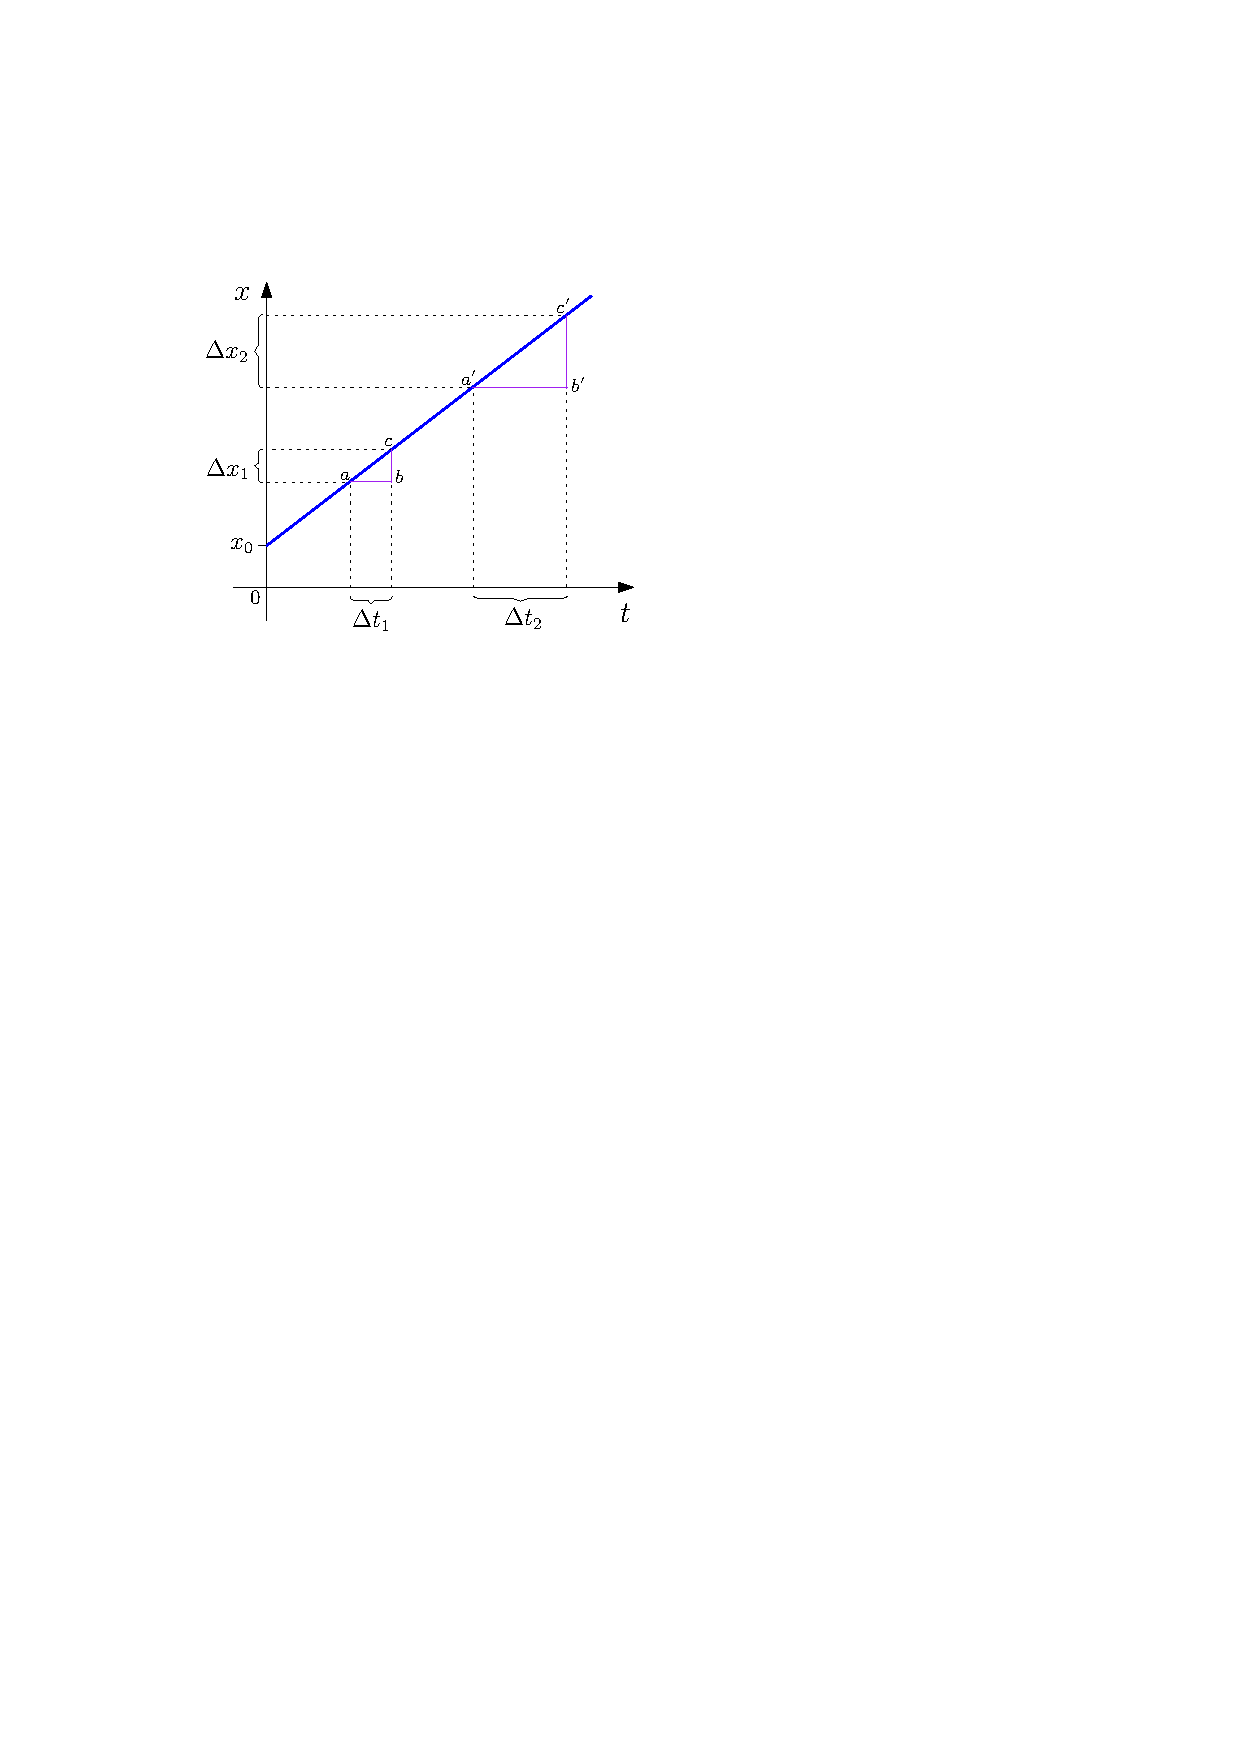
\includegraphics[scale=1]{img/MRU_intervalos.pdf}
  \end{center}
  ¿Qué tienen en común estos dos triángulos rectángulos? Dado que la rapidez es constante, podemos escribir
  $$v=\frac{\Delta x_1}{\Delta t_1}=\frac{\Delta x_2}{\Delta t_2}$$
  Es decir si dividimos {\it ``lo que varían las ordenadas''} por {\it ``lo que varían las absisas''} el cociente siempre es el mismo. Este cociente, constante para una recta, se llama {\bf pendiente}. Ahora podemos decir que, {\em en la gráfica $x=x(t)$ del MRU, la pendiente de la recta es la velocidad}.
\end{mybox}

\begin{comprension}
  \noindent
  {\bf Primero}  Analiza las siguientes gráficas:
  \begin{center}
    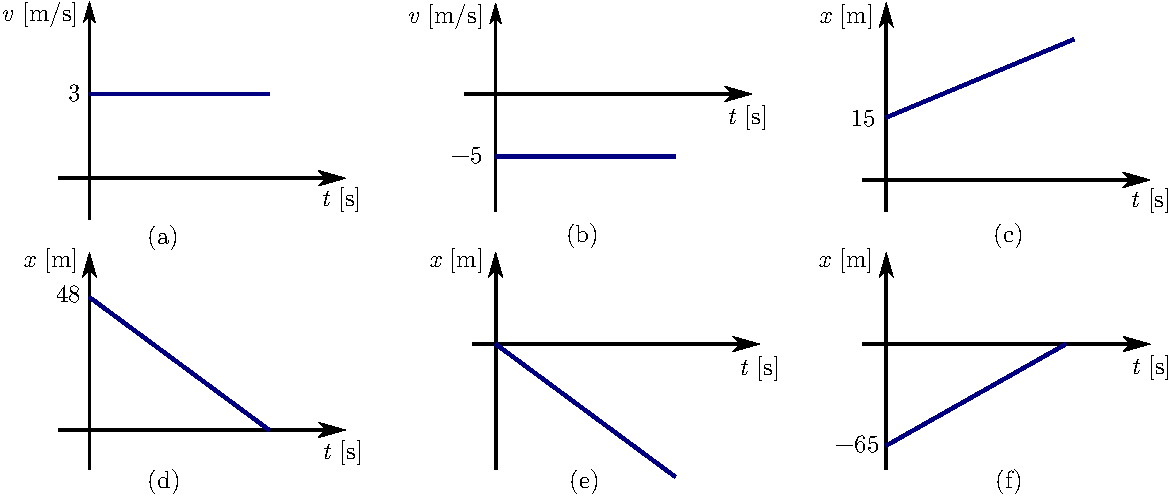
\includegraphics[width=0.9\textwidth]{img/analisisMRU.pdf}
  \end{center}

 \noindent
  {\bf Segundo} ¿Pueden la gráfica (b) y la (c) pertenecer a un mismo movimiento? Explica.
\end{comprension}


%% Acá va la sección de aceleración media e instantánea.
\section{Aceleración}
Cotidianamente podemos observar que los automóviles de las calles cambian su velocidad: frenan cuando llegan a una esquina (disminuyen su velocidad), aceleran luego de observar que es seguro cruzar la calle (aumentan su velocidad). En términos físicos, los automóviles {\it desaceleran} (frenan) cuando llegan a la esquina y luego {\it aceleran} para cruzar la calle. Que tan rápido varía la velocidad (disminución o aumento) en un instante (o intervalo) de tiempo, es lo que entiende la física por {\bf aceleración}.

\subsection{Aceleración media}

La {\bf aceleración media }se define como la razón entre la variación de velocidad $\mathbold{\Delta v}$ y el intervalo de tiempo $\Delta t$, en que se ha producido dicha variación:

\begin{center}
\boxed{\mathbold{\bar{a}_m}=\frac{\mathbold{\Delta \bar{v}}}{\Delta t}=\frac{\mathbold{\bar{v}}-\mathbold{\bar{v}_0}}{t-t_0}}
\end{center}

en donde dicha aceleración es una {\bf magnitud vectorial} la cual tiene la misma dirección y sentido que la variación de velocidad $\mathbold{\Delta \bar{v}}$, debido a que $\Delta t > 0$. 


Las unidades con que se miden las aceleraciones surgen, al igual que las velocidades, de la misma operación que las define. Se trata de un cociente entre una velocidad ($\Delta v$) y un intervalo de tiempo ($\Delta t$). Con esta expresión: $$[a_m] = \frac{[\Delta v]}{[\Delta t]}$$
Si trabajamos en el SIMELA, la unidad derivada es: $$[a_m] =\sif{$\!\!\sif{m}{s}$}{s} =\frac{\textrm{m}}{\textrm{s}^2}$$


{\bf \color{BrickRed} {¡Cuidado!}} En la vida cotidiana la palabra {\it aceleración} está asociada con el {\it movimiento}. Sin embargo, que un cuerpo no se esté acelerando o desacelerando, {\bf no implica que no se esté moviendo}. ¡Dicho cuerpo puede estar en movimiento con velocidad constante!
\\


Veamos gráficamente un caso rectilíneo en donde un automóvil que recorre el trayecto $P_0$ - $P$, cambia desde una velocidad $\mathbold{\bar{v}_0}$ hasta una velocidad $\mathbold{\bar{v}}$ de mayor módulo en un intervalo de tiempo $\Delta t$

\begin{figure}[!h]
\centering
 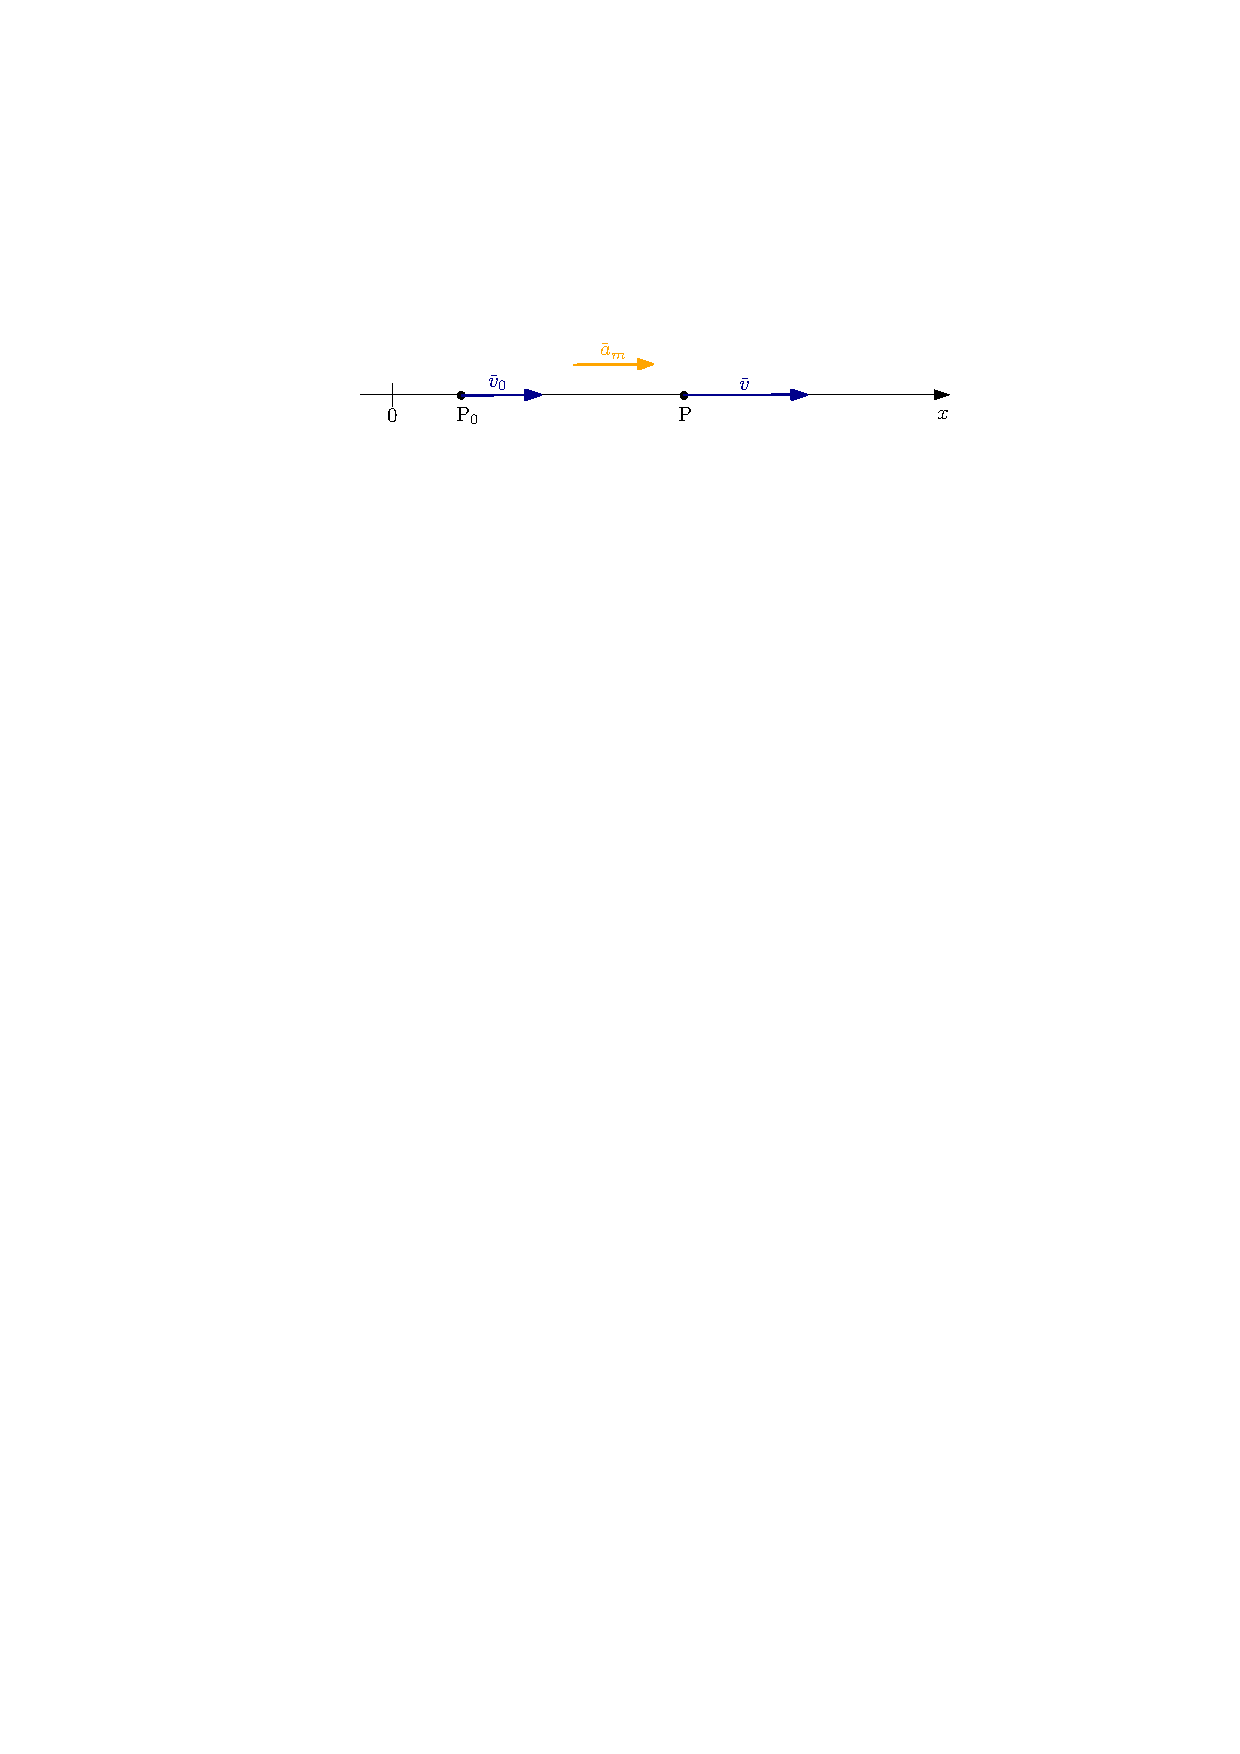
\includegraphics[width=.6\textwidth]{img/amedia.pdf}
 \caption{Aceleración media en un movimiento rectilíneo.}
\end{figure}


Como ya se dijo, la aceleración es una magnitud vectorial. Pensemos en dos automóviles que están acelerando  uniformemente por la misma ruta en sentidos opuestos a 5\,km/h$^2$ y 10\,km/h$^2$, respectivamente. Teniendo en cuenta el sistema de coordenadas estas aceleraciones resultarán de signo opuesto:



\begin{figure}[!h]
\centering
 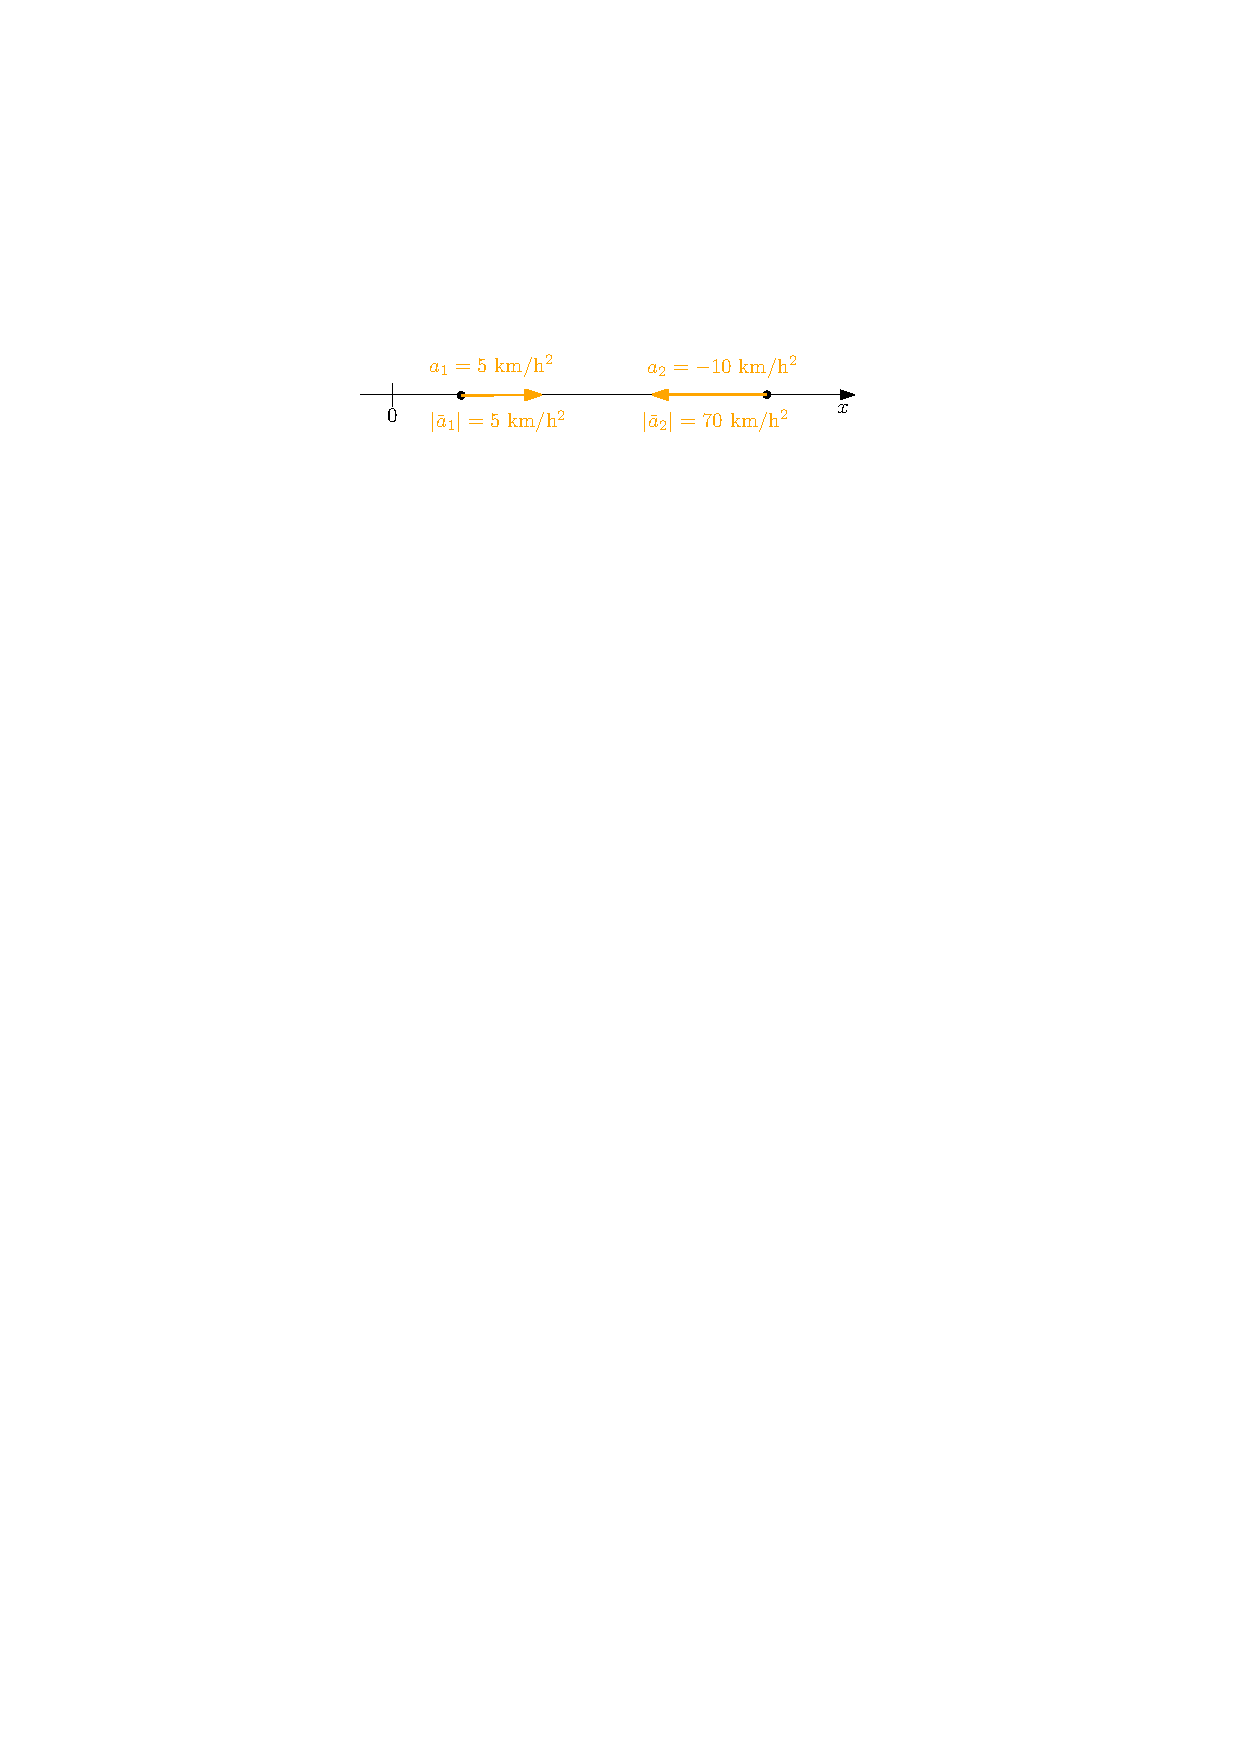
\includegraphics[width=.6\textwidth]{img/acomp1.pdf}
% \caption{Aceleración media en un movimiento rectilíneo.}
\end{figure}

El signo de la aceleración \textbf{depende del sistema de coordenadas}.


{\bf \color{BrickRed} {¡Cuidado!}} En el ejemplo anterior, al igual que acurre con la velocidad, cuando decimos ``$a_1= 5$ km/h'' o ``$a_2= -10$ km/h'', {\bf ¡nos estamos refiriendo a la componente $x$ del vector aceleración!} Debido a que el movimiento es rectilíneo, es decir que la partícula se mueve en el eje $x$, podemos utilizar esta notación. Si el movimiento fuera en un plano deberíamos escribir sus dos componentes:

\begin{figure}[h!]
\centering
 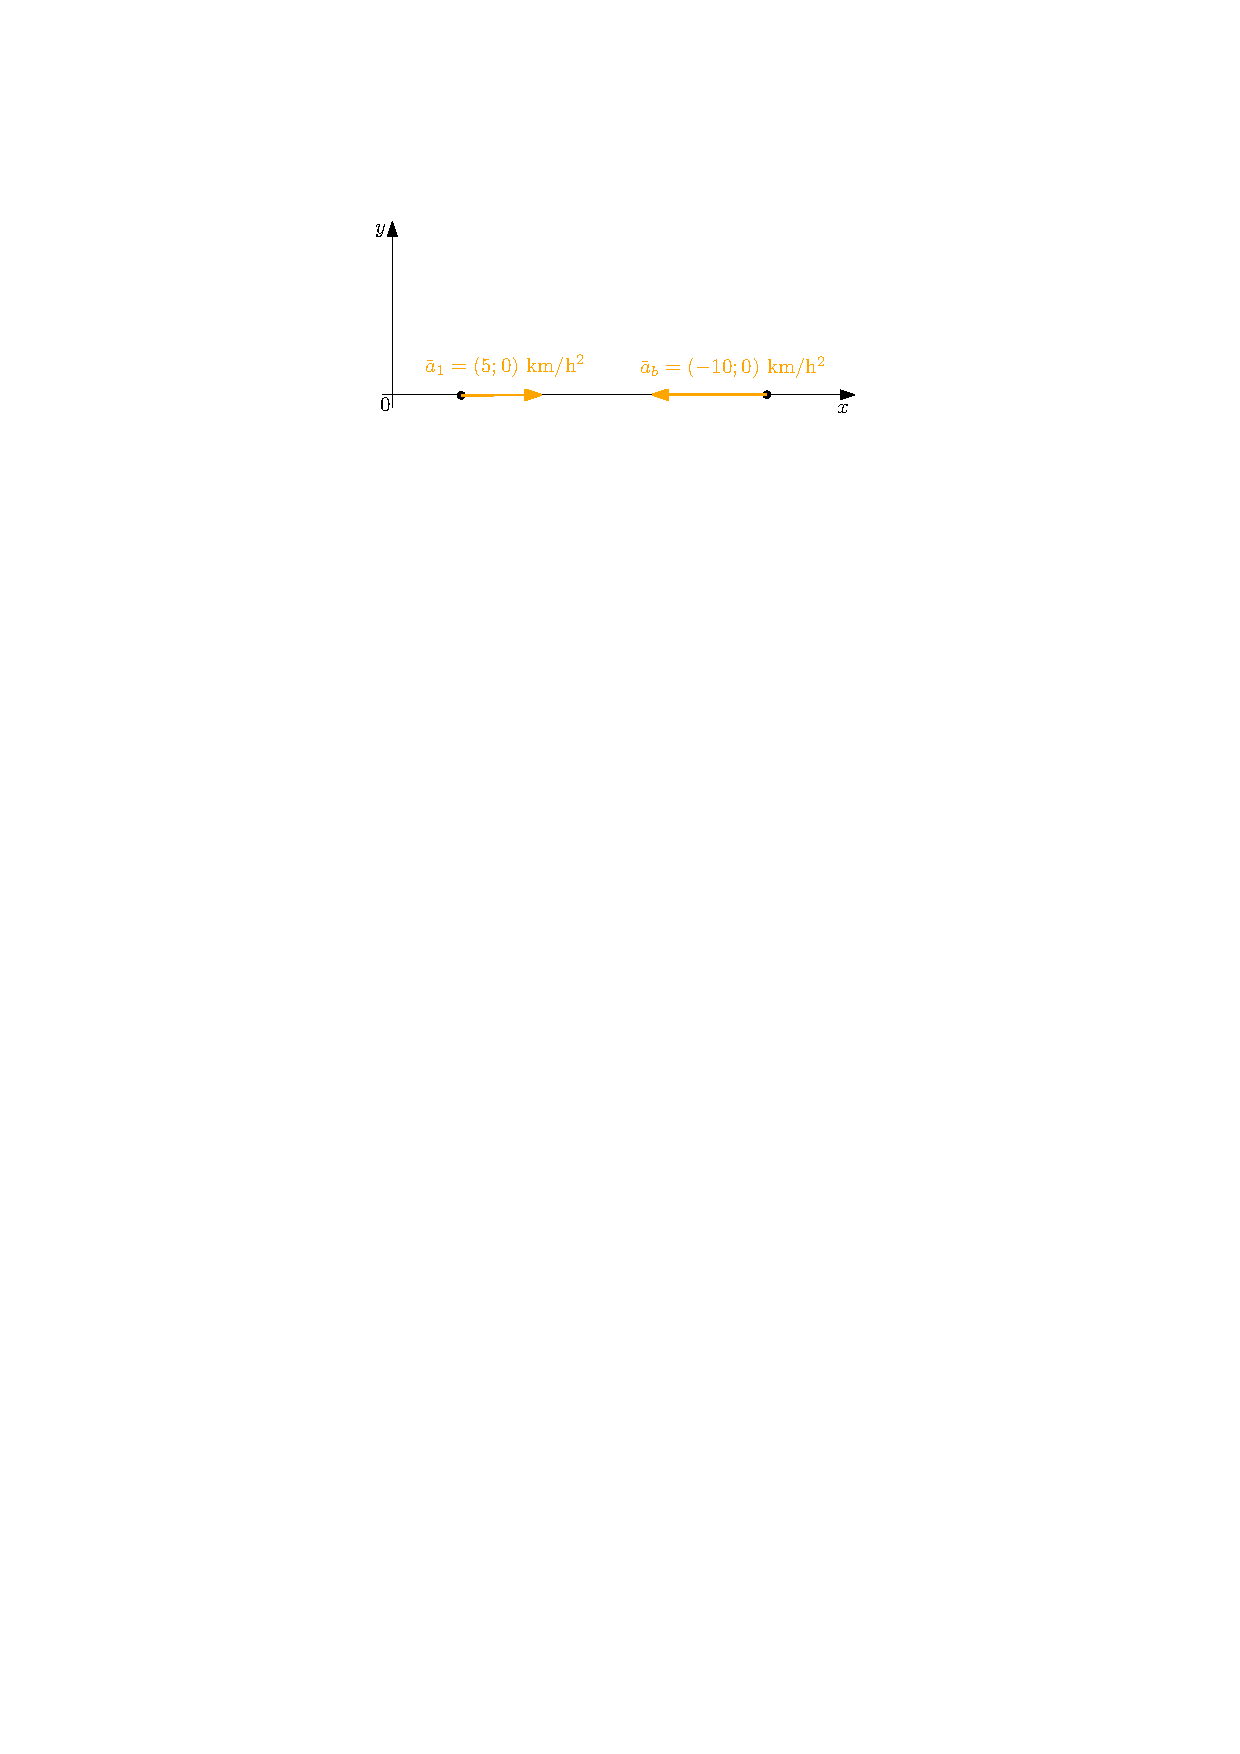
\includegraphics[width=.6\textwidth]{img/acomp2.pdf}
 % \caption{Velocidad media en un movimiento rectilíneo.}
\end{figure}



Retomando el análisis del principio de la sección, si decimos que un objeto {\it acelera} o {\it desacelera}, nos estamos refiriendo a cómo varía la rapidez, sin pensar en la dirección o el sentido de la velocidad. 

¿Cómo sabemos si una partícula está \textit{acelerando} o \textit{desacelerando}?

\info{
    Contrario a lo que se tiende a pensar, no es el signo de la aceleración por sí solo el que indica si una partícula \textit{acelera} o \textit{desacelera}.}
    
Podremos saber si un objeto está acelerando o desacelerando comparando el signo de la velocidad con el signo de la aceleración. ¿Cómo es esto? Debemos tener presente que \textbf{la aceleración nos indica cómo cambia la velocidad}, si la aceleración apunta en el mismo sentido que la velocidad, esta aumentará su módulo pero si, por el contrario, ambas apuntan en sentido opuesto, la velocidad disminuirá su módulo.

En los cuatro ejemplos de la Figura siguiente se observan las posibles combinaciones de $\mathbold{\bar{v}}$ y $\mathbold{\bar{a}}$ que podemos tener, todas para un mismo sistema de referencia.

\begin{figure}[H]
 \begin{subfigure}{0.5\textwidth}
    \centering
 	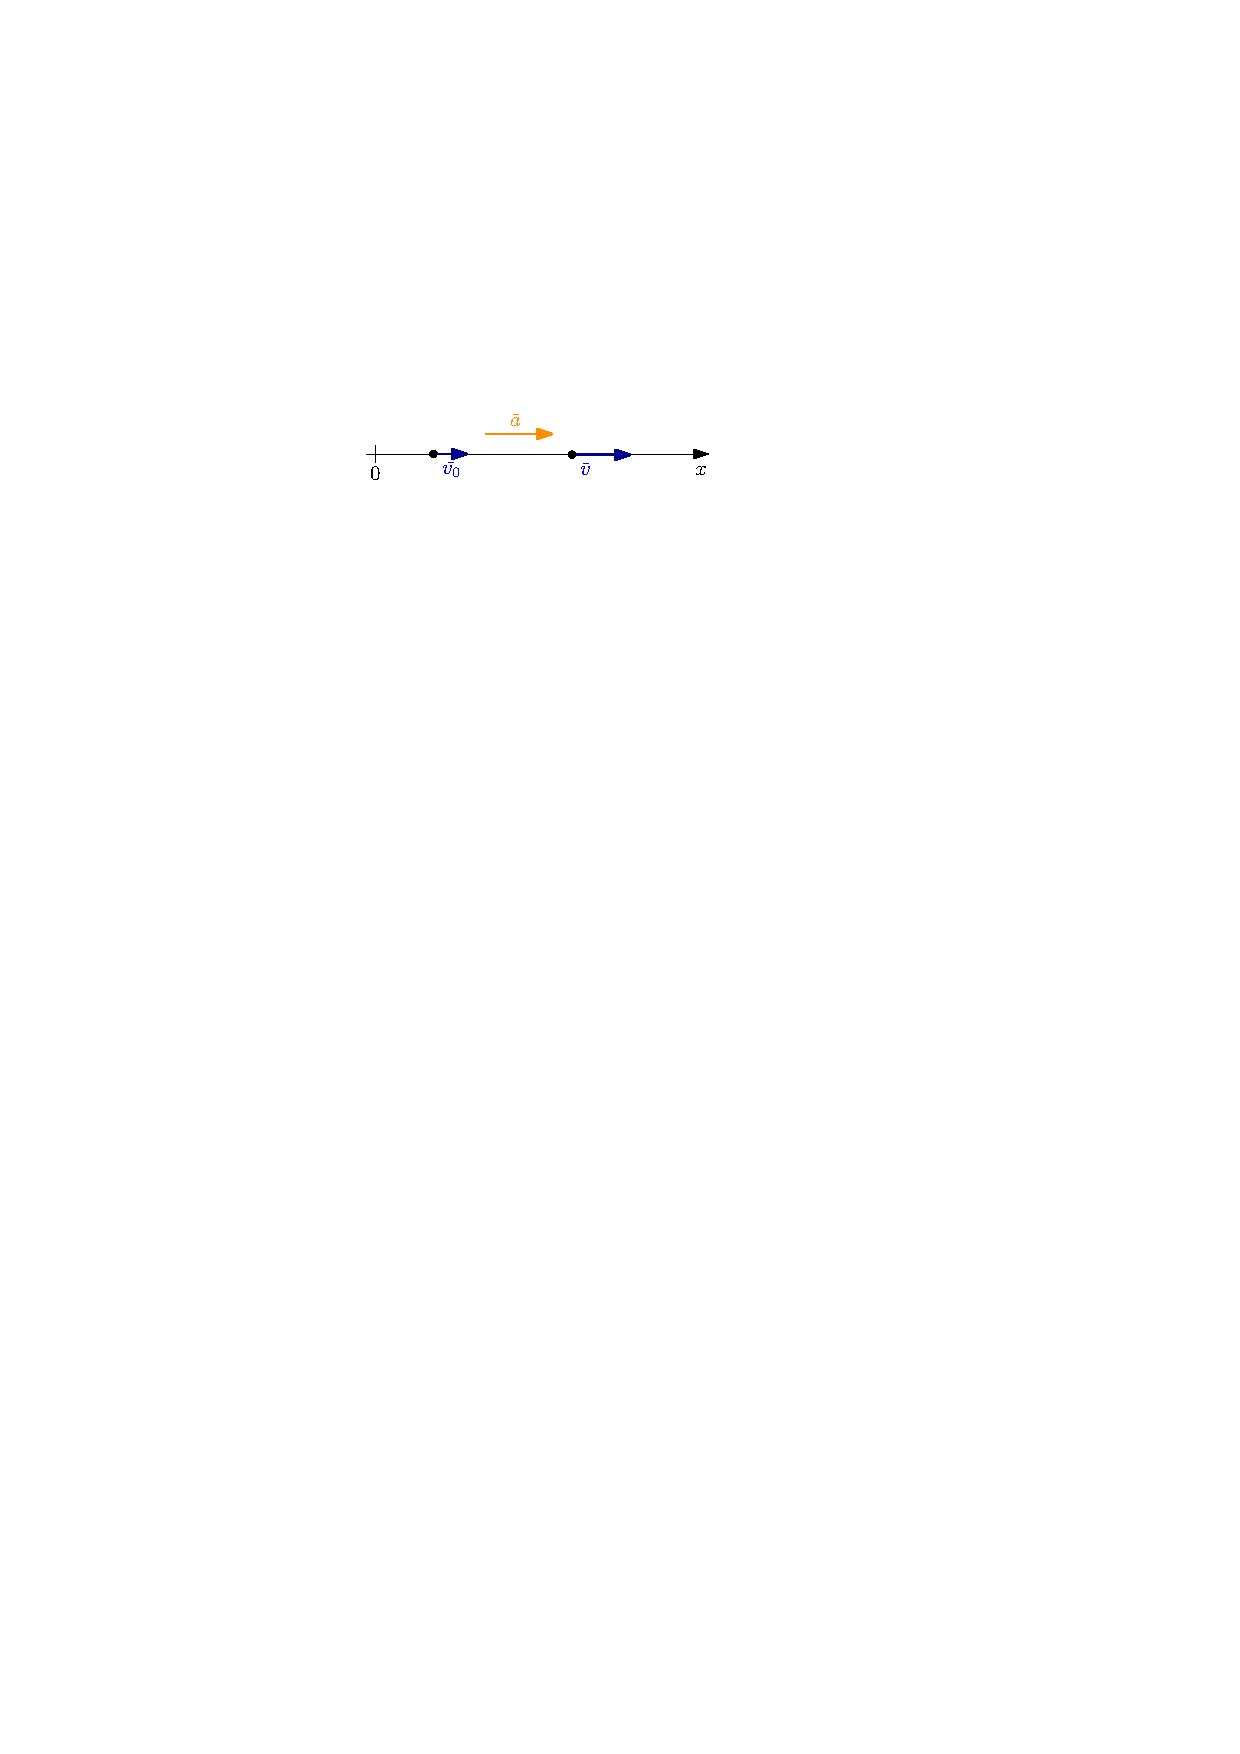
\includegraphics[width=.9\linewidth]{img/acelera1.pdf}
	\caption{$a>0$ y  \textit{acelera}}	
\end{subfigure}   
 \begin{subfigure}{0.5\textwidth}
    \centering
 	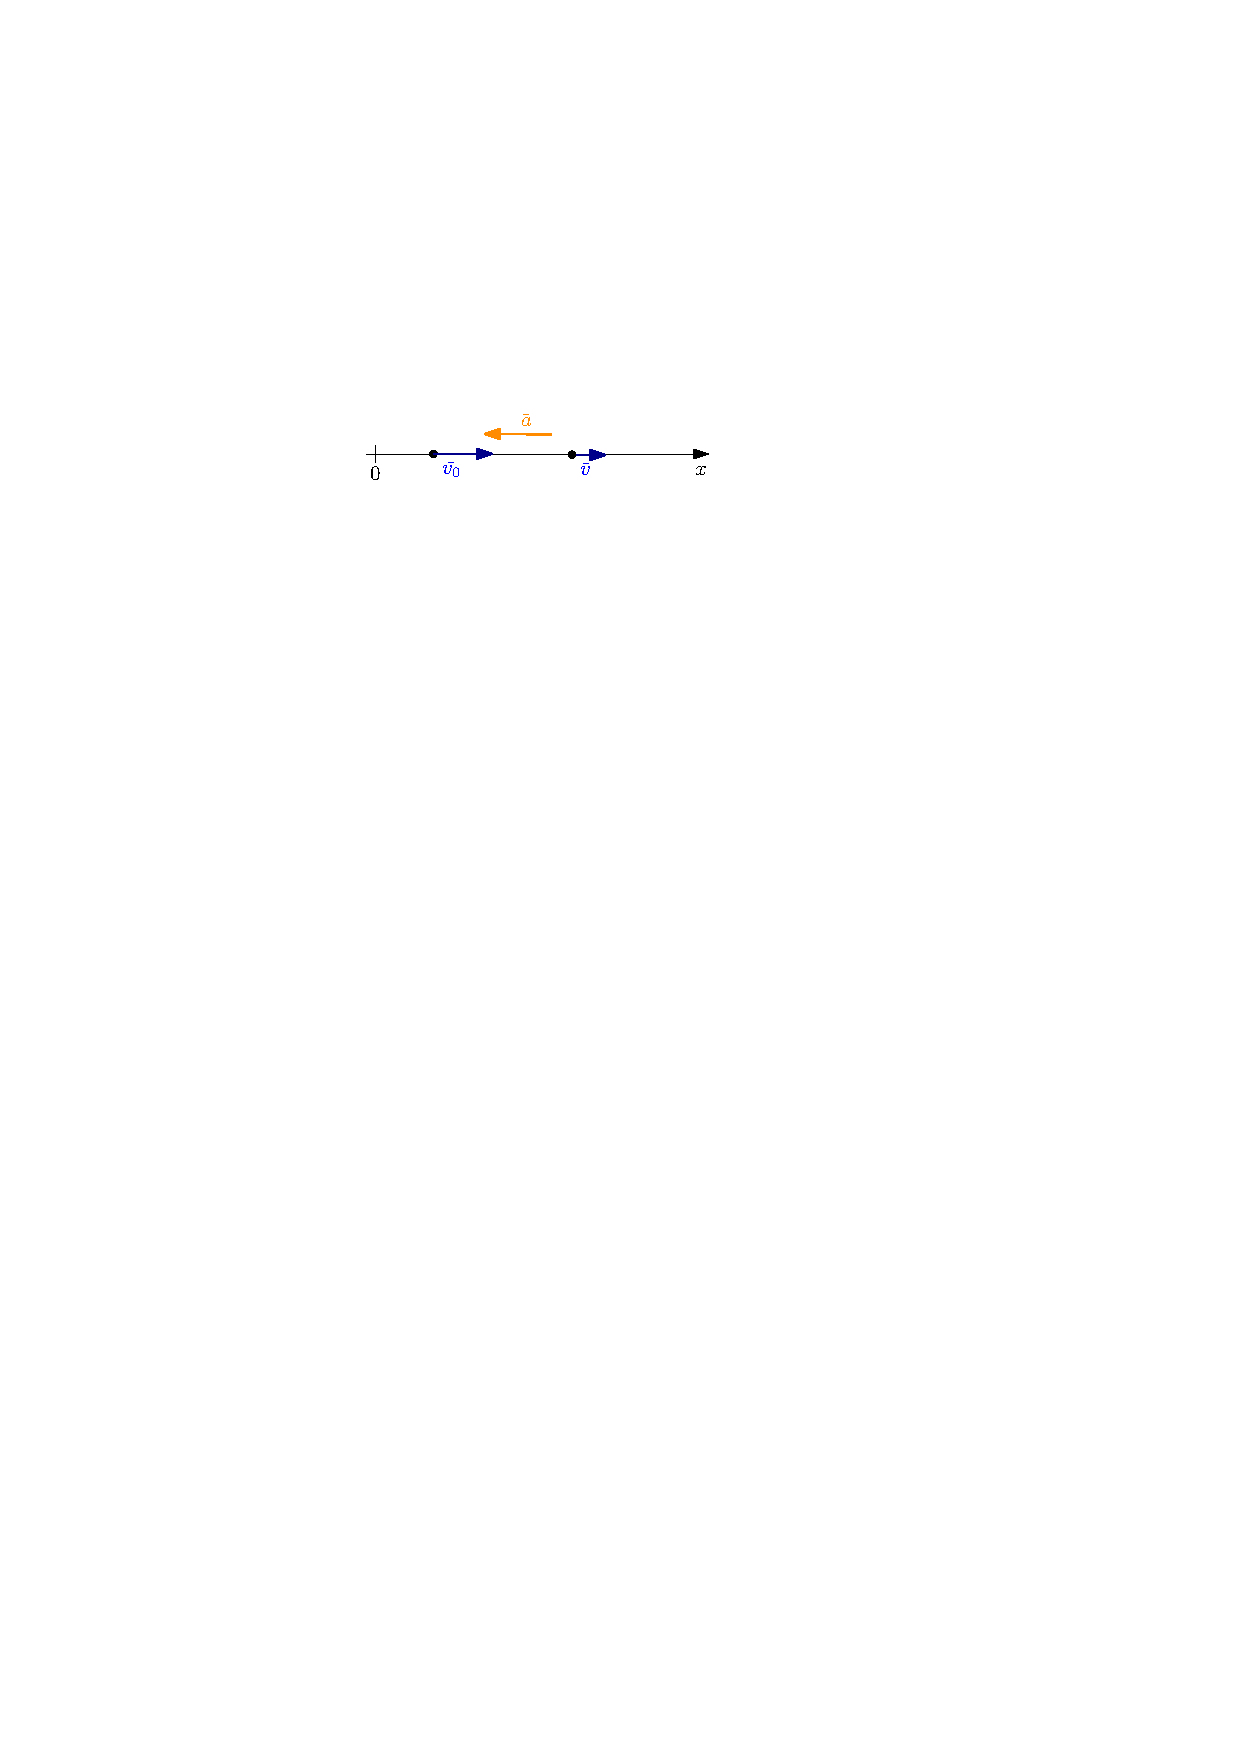
\includegraphics[width=.9\linewidth]{img/acelera2.pdf}
	\caption{$a<0$ y \textit{desacelera}}	
\end{subfigure}
 \begin{subfigure}{0.5\textwidth}
    \centering
 	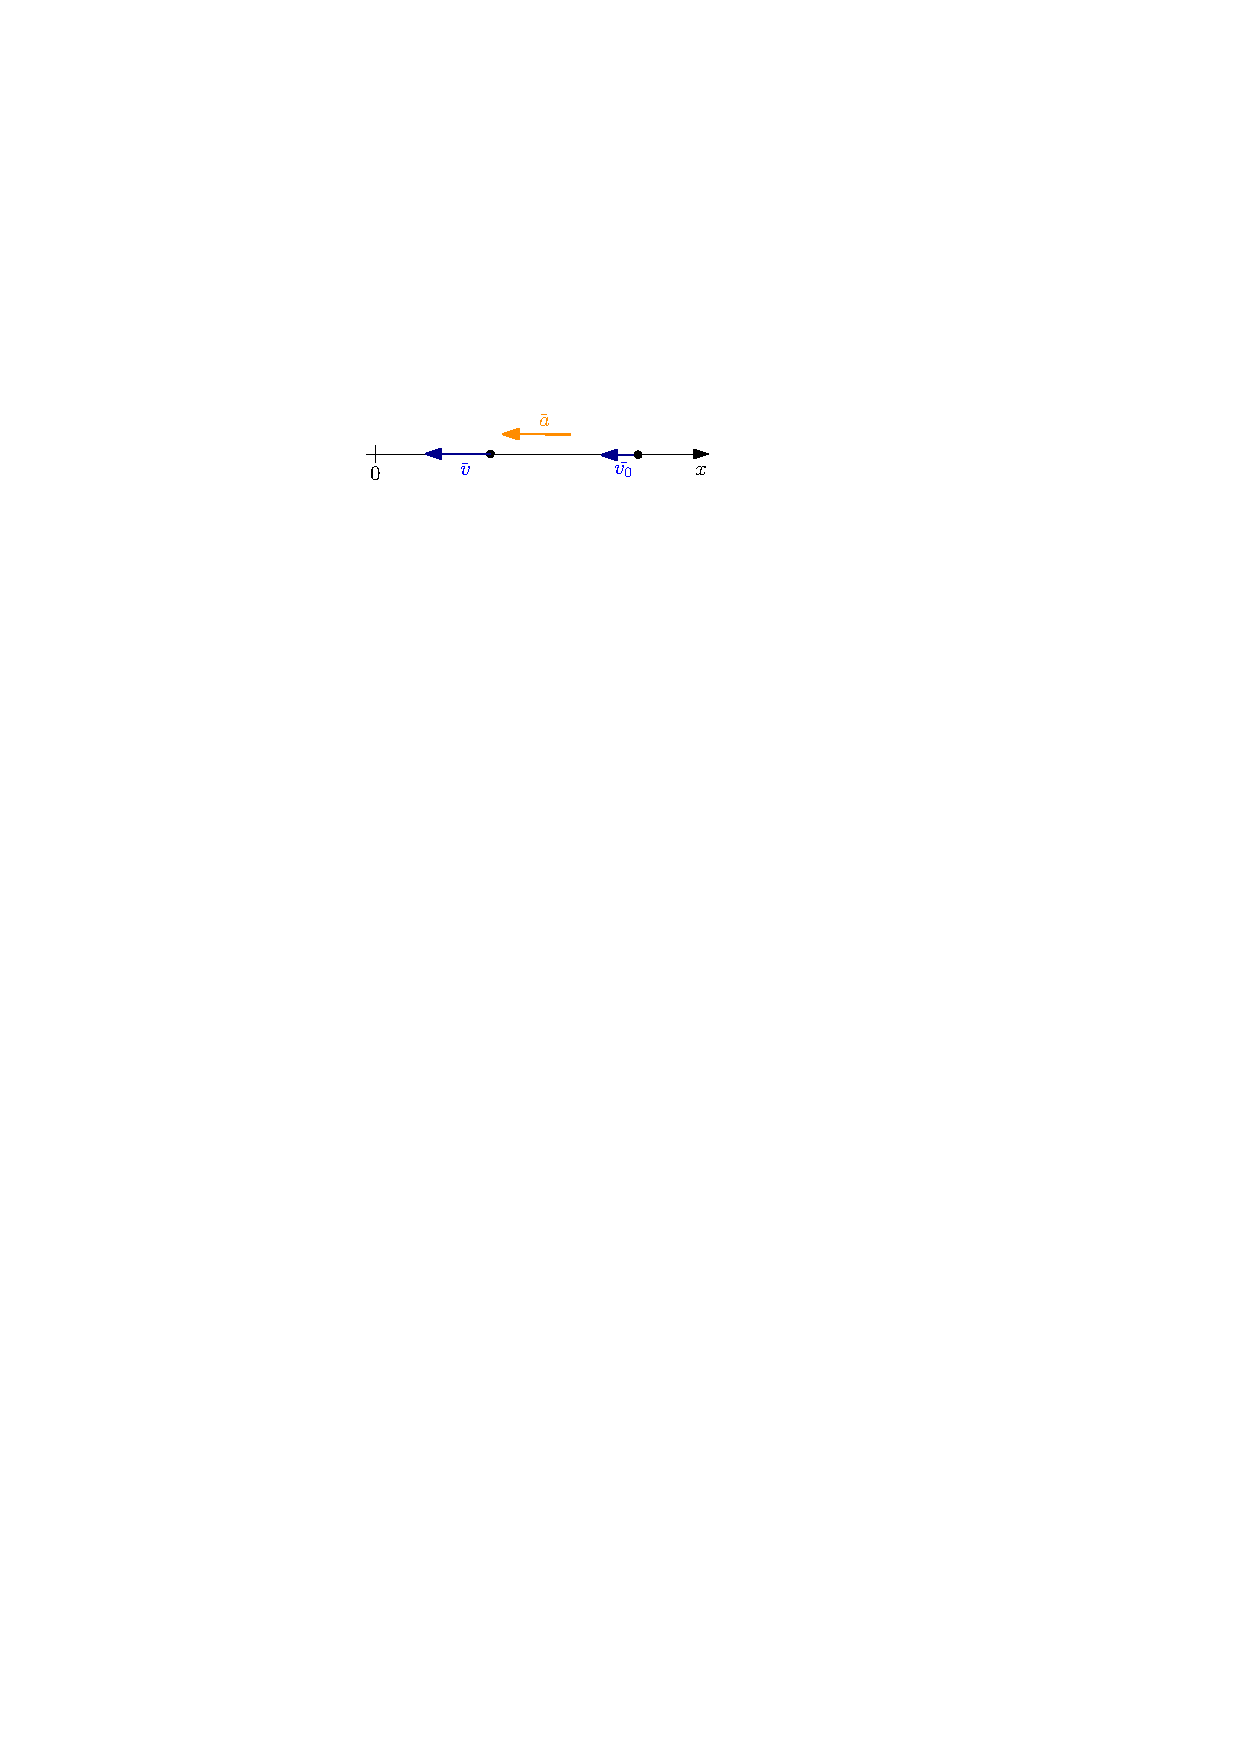
\includegraphics[width=.9\linewidth]{img/acelera3.pdf}
	\caption{$a<0$ y \textit{acelera}}	
\end{subfigure} 
 \begin{subfigure}{0.5\textwidth}
    \centering
 	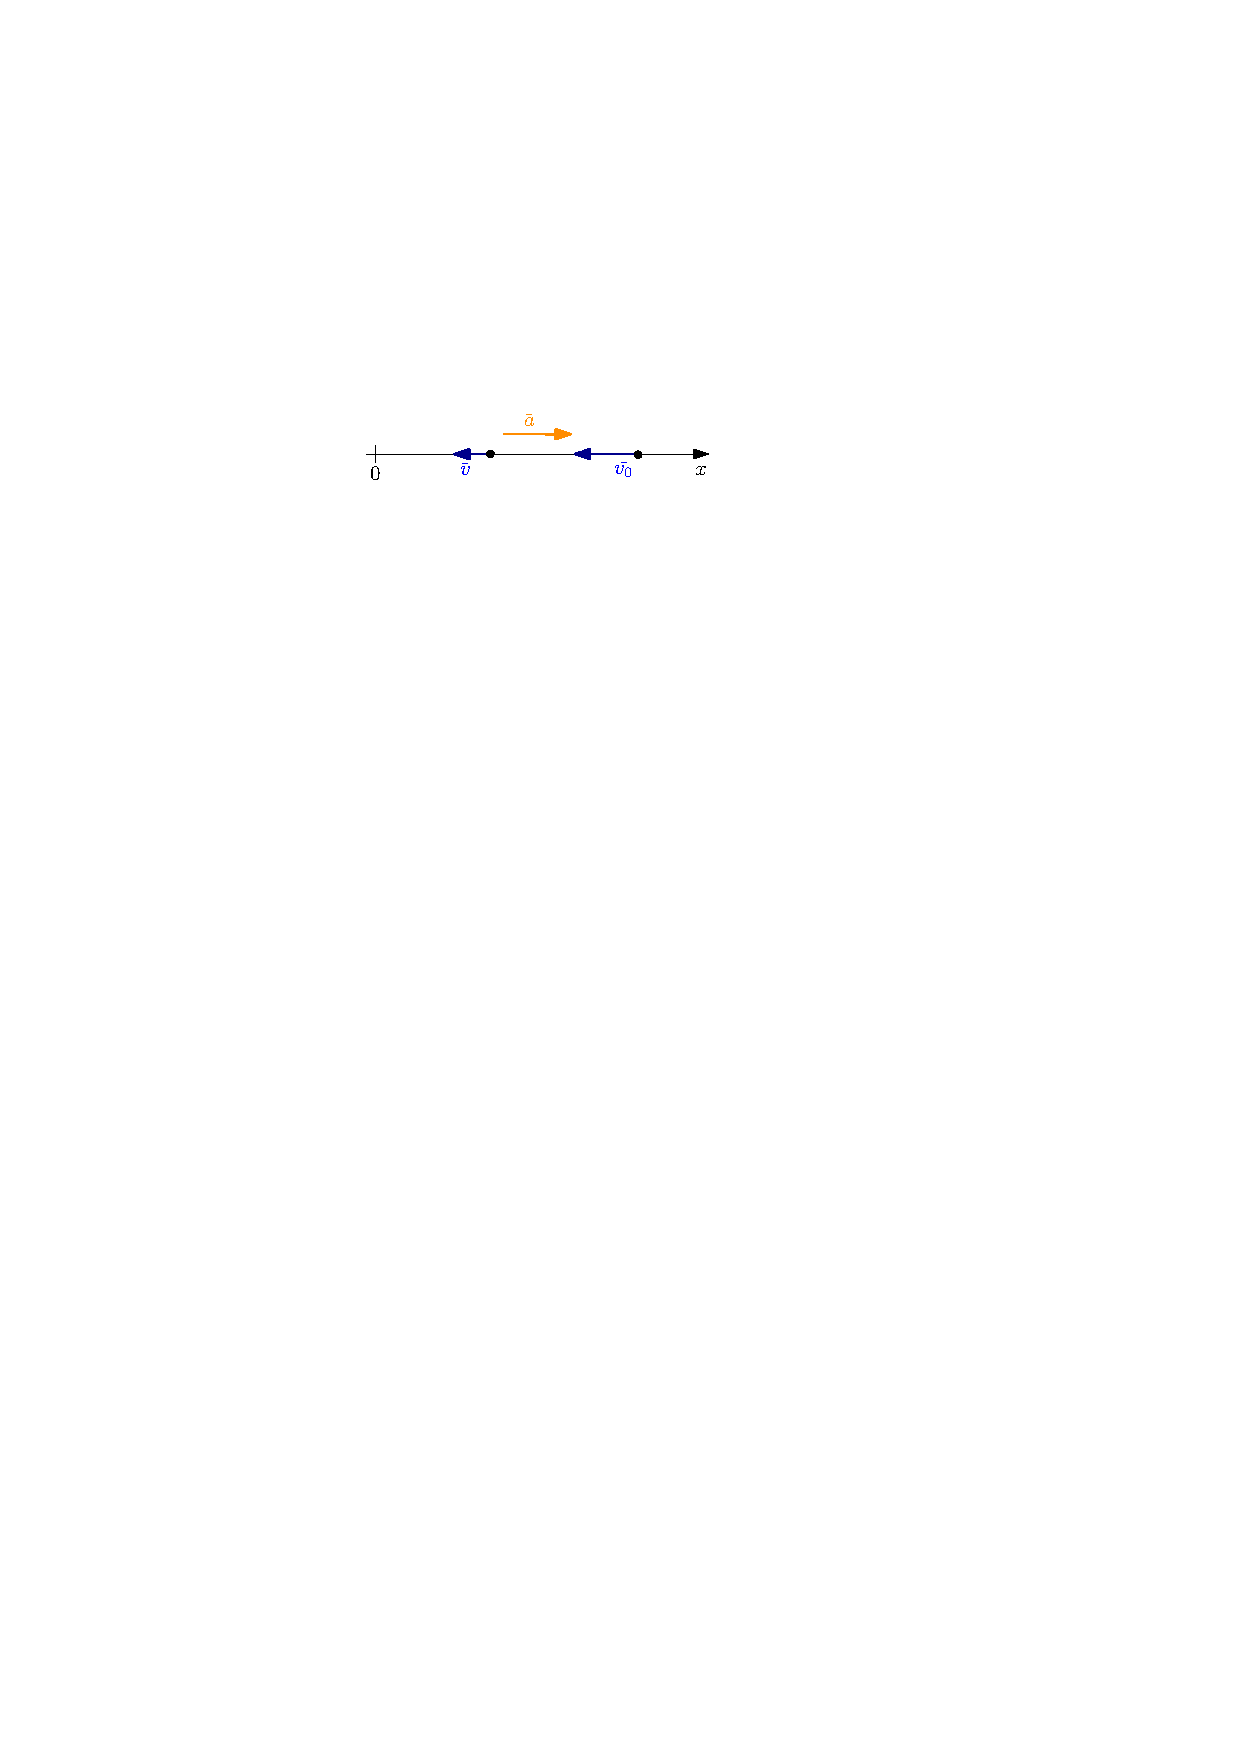
\includegraphics[width=.9\linewidth]{img/acelera4.pdf}
	\caption{$a>0$ y \textit{desacelera}}	
\end{subfigure} 
\end{figure}








\info{

Si viajamos en un automóvil que se mueve con velocidad constante, sin la posibilidad de mirar hacia afuera, nos es {\it imposible} decir que dicho automóvil está en movimiento o en reposo. En otras palabras {\bf ¡no podemos percibir la velocidad!} En cambio, si éste aumenta su velocidad (acelera), experimentamos dicho aumento al recargarnos más contra los asientos. Y si disminuye su velocidad (desacelera), nos despegamos de dichos asientos. En otras palabras {\bf ¡podemos percibir la aceleración!}}



Recordemos que la velocidad también es una magnitud vectorial. Por lo tanto un cambio en la velocidad $\mathbf{\Delta \bar{v}}$ implica que la misma puede haber cambiado su:
\begin{itemize}
\item {\bf módulo} (rapidez)
\item {\bf dirección}
\item {\bf sentido}
\end{itemize}


\begin{comprension}
¿Puede un móvil realizar un movimiento con rapidez constante aún cuando su velocidad varía?\\
{\em Ayuda: Piensa en un movimiento en el plano.}
\end{comprension}


Dado su carácter vectorial, la aceleración es entonces un concepto que contempla:

\subsubsection{Cambio en el módulo de la velocidad}

\begin{figure}[H]
\centering
 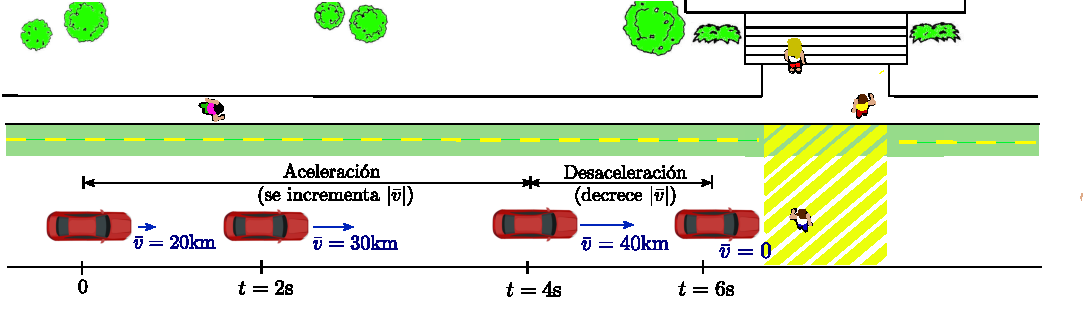
\includegraphics[width=1.1\textwidth]{img/auto1.pdf}
 \caption{Aceleración debido a la variación del módulo de la velocidad.}
\end{figure}

\subsubsection{Cambio en la dirección o el sentido de la velocidad}

\begin{figure}[H]
\centering
 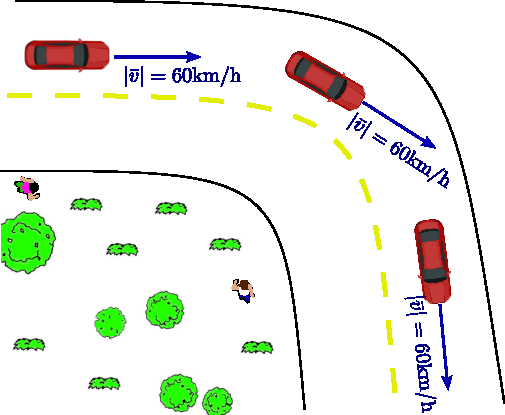
\includegraphics[width=.5\textwidth]{img/auto2.pdf}
 \caption{Aceleración debido al cambio en la dirección de la velocidad.}
\end{figure}


\subsection{Aceleración instantánea}

En algunas situaciones el valor de la aceleración media puede ser diferente en intervalos de tiempo distintos. Por este motivo es útil definir la {\bf aceleración instantánea}, como hicimos anteriormente con la velocidad instantánea:


$$\mathbold{\bar{a}}= \lim_{\Delta t \rightarrow 0} \mathbold{\bar{a}_m} = \lim_{\Delta t \rightarrow 0} \frac{\mathbold{\Delta \bar{v}}}{\Delta t}$$

%% Acá va la sección de MRUV
\section{Movimiento Rectilíneo Uniformemente Variado}
Como ya anticipamos, el otro movimiento que estudiaremos es el \textbf{Movimiento Rectilíneo Uniformemente Variado (MRUV)}. \textbf{Este es un movimiento con aceleración constante en una trayectoria rectilínea.}

En este caso la partícula se mueve en línea recta modificando uniformemente su velocidad: se producen iguales cambios de velocidad en iguales intervalos de tiempo (ya que $\bar{a} = cte$). Recordando que la aceleración es un cambio en la velocidad (¡que es un vector!), vale aclarar que en el MRUV no cambia la dirección de la velocidad sino su módulo y eventualmente su sentido.

Como la aceleración es constante, la aceleración media es igual a la aceleración instantánea, y por lo tanto la velocidad varía (aumenta o disminuye) igual cantidad en
iguales intervalos de tiempo.

Como la aceleración media y la aceleración instantánea son iguales:
$$\mathbf{\bar{a}}=\mathbold{\bar{a}_m}=\frac{\mathbold{\Delta \bar{v}}}{\Delta t}=\frac{\bar{v}-\bar{v_0}}{t-t_0}$$

Trabajando la expresión anterior por componentes queda: $\displaystyle {a}=\frac{{v}-{v_0}}{t-t_0}$,
que se puede reescribir como
$${a}(t-t_0) = {v} - {v_0}$$
De donde
\begin{center}
{\color{NavyBlue}  \boxed{\mathbold{v = v_0 + a \Delta t}}}
\end{center}
Esta expresión tiene la misma {\it forma} que la {\em ``Ley de movimiento del MRU''}. Nótese qué significa esto: en el MRU la posición variaba uniformemente; en el MRUV la velocidad es la que varía uniformemente.

Si $t_0=0$, entonces:
$${v}={v}_0+{a}t$$

¿Cómo determinamos la posición de una partícula en cada instante de tiempo para un MRUV? Sería interesante, al igual que para el MRU, encontrar una \textit{Ley de movimiento}. Para ello, recordemos que si una partícula se mueve con velocidad de módulo constante $v_0$, desde el instante de tiempo $t_0$ al instante $t$, el desplazamiento $\Delta x$ viene dado por:
$$\Delta x = v_0 (t-t_0)=v_0 \Delta t$$

Si representamos gráficamente la velocidad en función del tiempo (Figura \ref{fig:area}), podemos ver que $v_0 \Delta t$ es el área que queda debajo de la gráfica: el área de un rectángulo. Se puede probar que esto no es casualidad y que el desplazamiento siempre es el área debajo de la línea (en general decimos \textit{curva}) que representa la velocidad en función del tiempo.

\begin{figure}[!h]
\centering
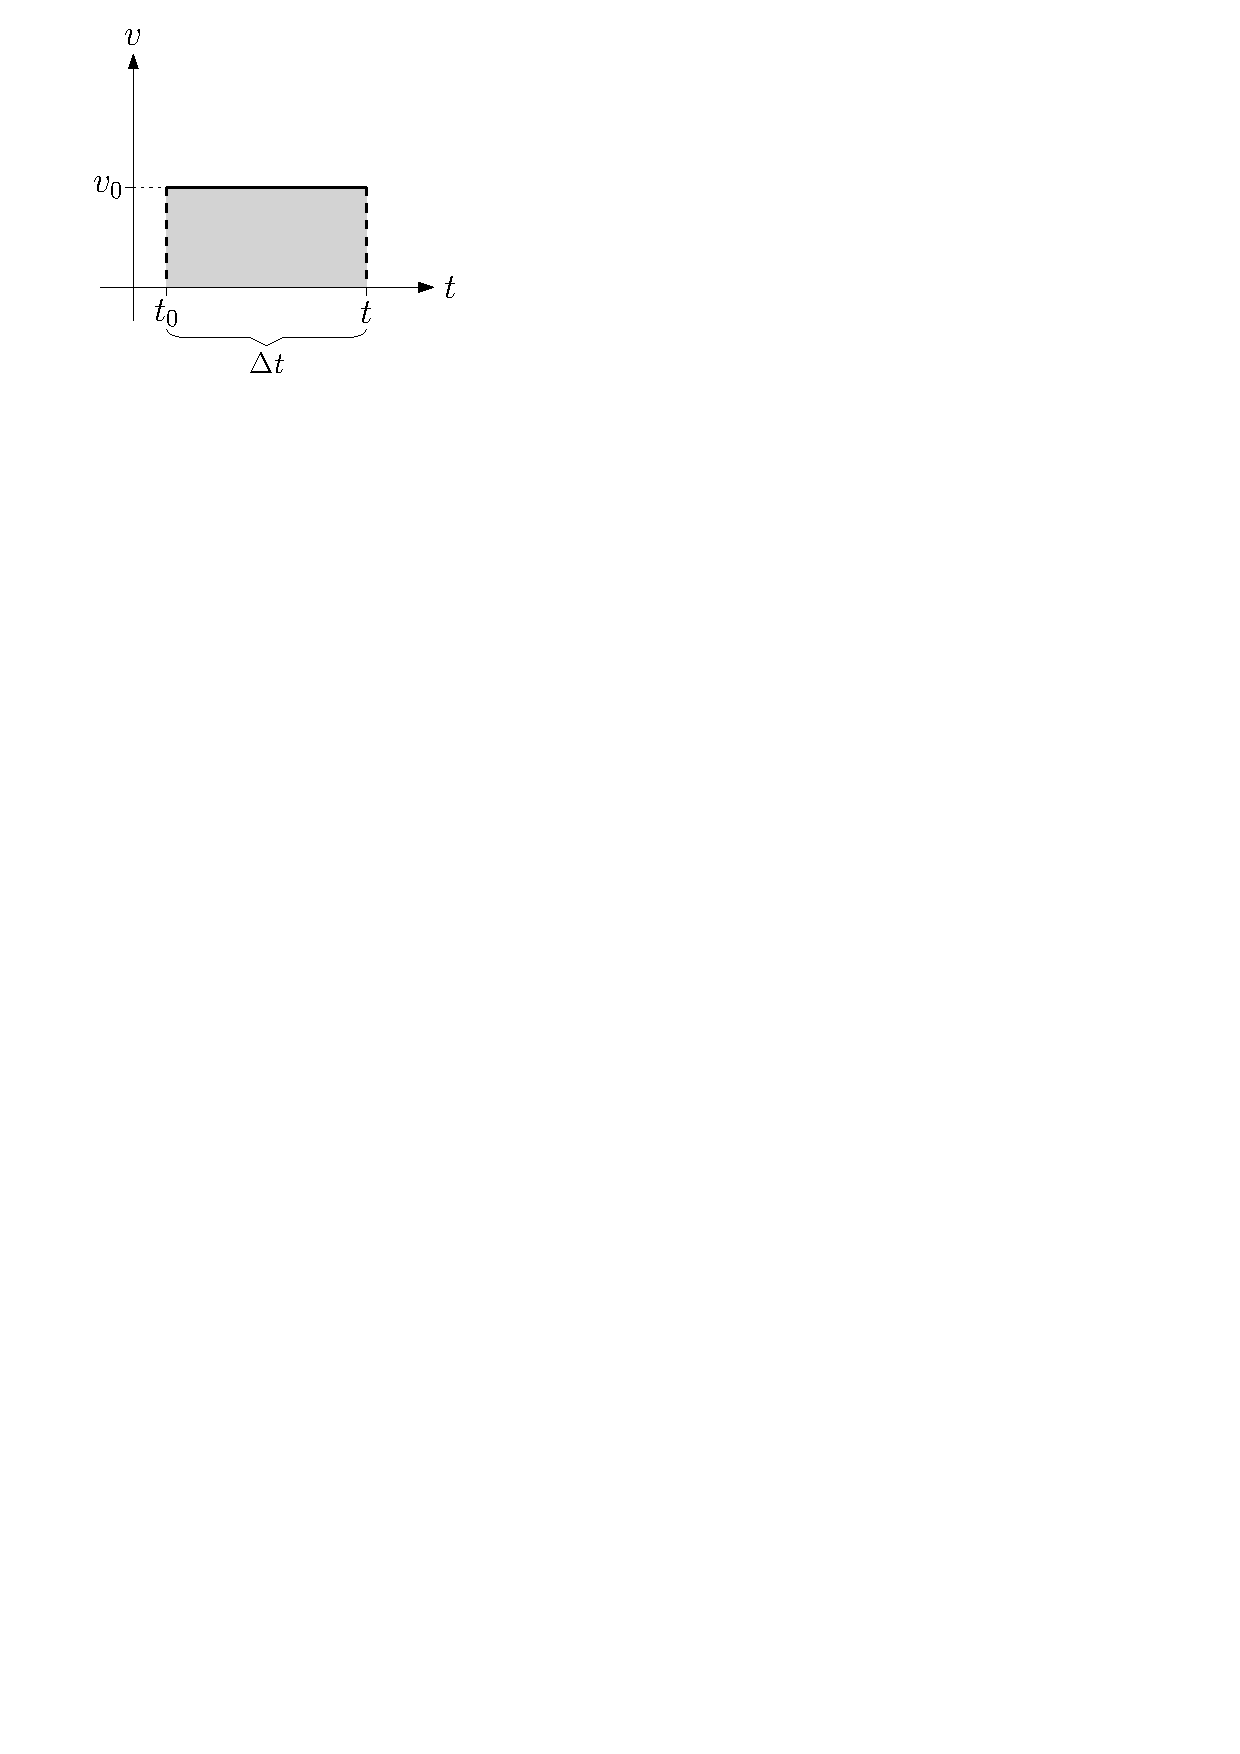
\includegraphics{img/area.pdf}
\caption{Gráfica de velocidad en función del tiempo para un MRU, el desplazamiento es el área marcada en gris}
\label{fig:area}
\end{figure}

La gráfica de la velocidad en función del tiempo para un MRUV se muestra en la Figura \ref{fig:area2}.

\begin{figure}[!h]
\centering
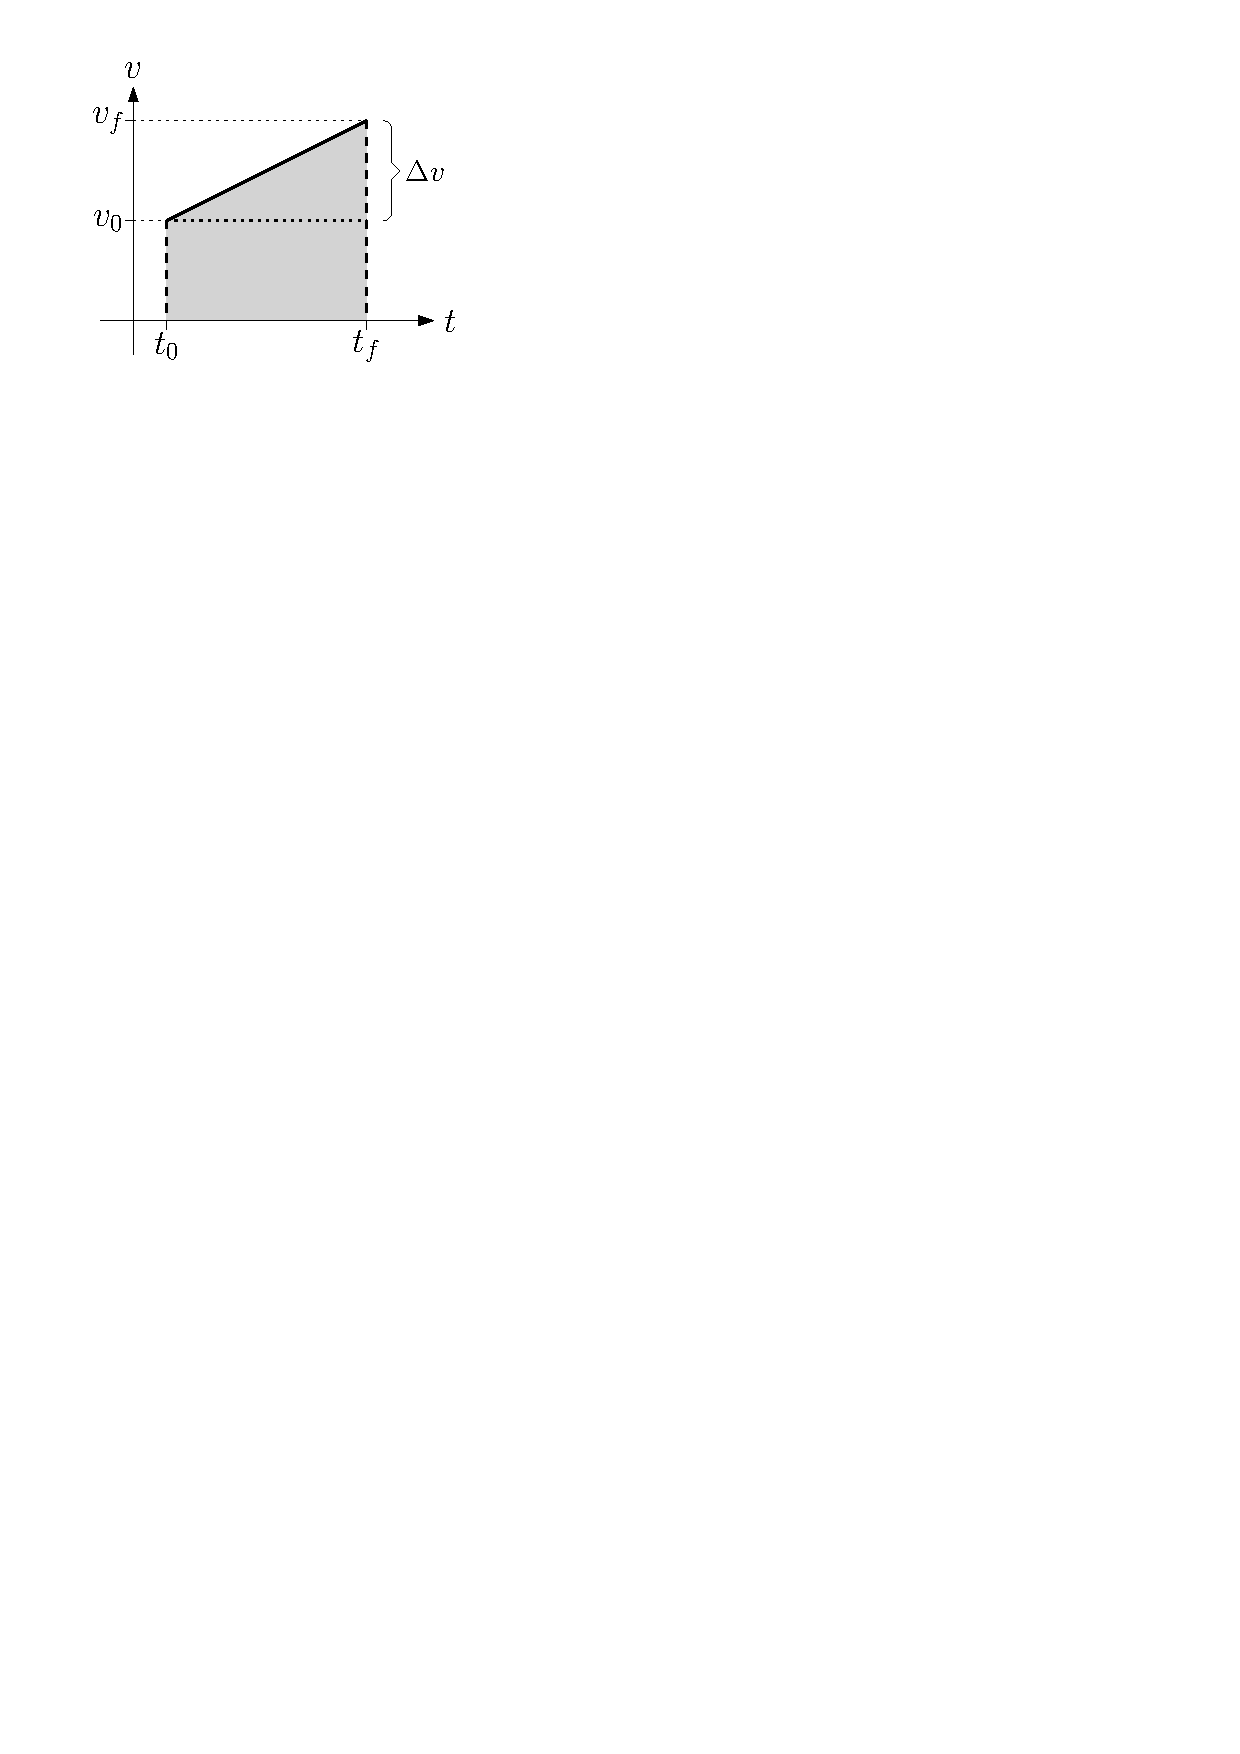
\includegraphics{img/area2.pdf}
\caption{Gráfica de velocidad en función del tiempo para un MRUV, el desplazamiento será el área en gris}
\label{fig:area2}
\end{figure}

Para calcular el área debajo de la curva podemos pensar que se compone de dos partes: un rectángulo y un triángulo.
\begin{eqnarray*}
\Delta x & = & \mbox{área }\square + \mbox{área } \triangle \\
& = & v_0(t-t_0) + \frac{1}{2} (v-v_0) (t-t_0) 
\end{eqnarray*}
Si multiplicamos y dividimos el último término por $(t-t_0)$
\begin{eqnarray*}
\Delta x & = & v_0(t-t_0) + \frac{1}{2} \overbrace{\frac{(v-v_0)}{\textcolor{red}{(t-t_0)}}}^{\displaystyle\textcolor{orange}{a}} (t-t_0) \textcolor{red}{(t-t_0)} \\
 & = & v_0 \Delta t  +  \frac{1}{2} a (\Delta t)^2 \\
x-x_0 & = & v_0 \Delta t + \frac{1}{2} a (\Delta t)^2
\end{eqnarray*}
De donde se obtiene:
\begin{center}
{\color{ForestGreen}  \boxed{\mathbold{x=x_0+v_0\Delta t+\frac{1}{2}a(\Delta t)^2}}}
\end{center}

Tal como planteamos originalmente, la expresión de $x-x_0$ tiene dos términos: $v_0\Delta t$ que ya aparecía en la ley de movimiento del MRU y el término $\frac{1}{2}a(\Delta t)^2$ que habla del desplazamiento adicional debido al cambio de velocidad. En otras palabras, una partícula que se mueve aumentando su velocidad se desplaza \textit{un poco más} que una que se mueve a velocidad constante.

Nótese que si $a=0$ estamos hablando de un MRU y la ecuación anterior se transforma en la que ya conocíamos:
$$x=x_0+v\Delta t$$

En muchas situaciones de interés, la \textit{Ley de movimiento del MRUV} se puede simplificar tomando $t_0=0$, y así nos queda $$x=x_0+v_0t+\frac{1}{2}at^2$$

\begin{mybox}{Para profundizar}

¿Por qué siempre el área bajo la curva de velocidad en función del tiempo es el desplazamiento? La idea de \textit{área bajo la curva} tiene muchas aplicaciones en Física. Si bien la justificación de esta idea excede el contenido de este curso, daremos una pequeña noción al respecto.

\begin{center}
\centering
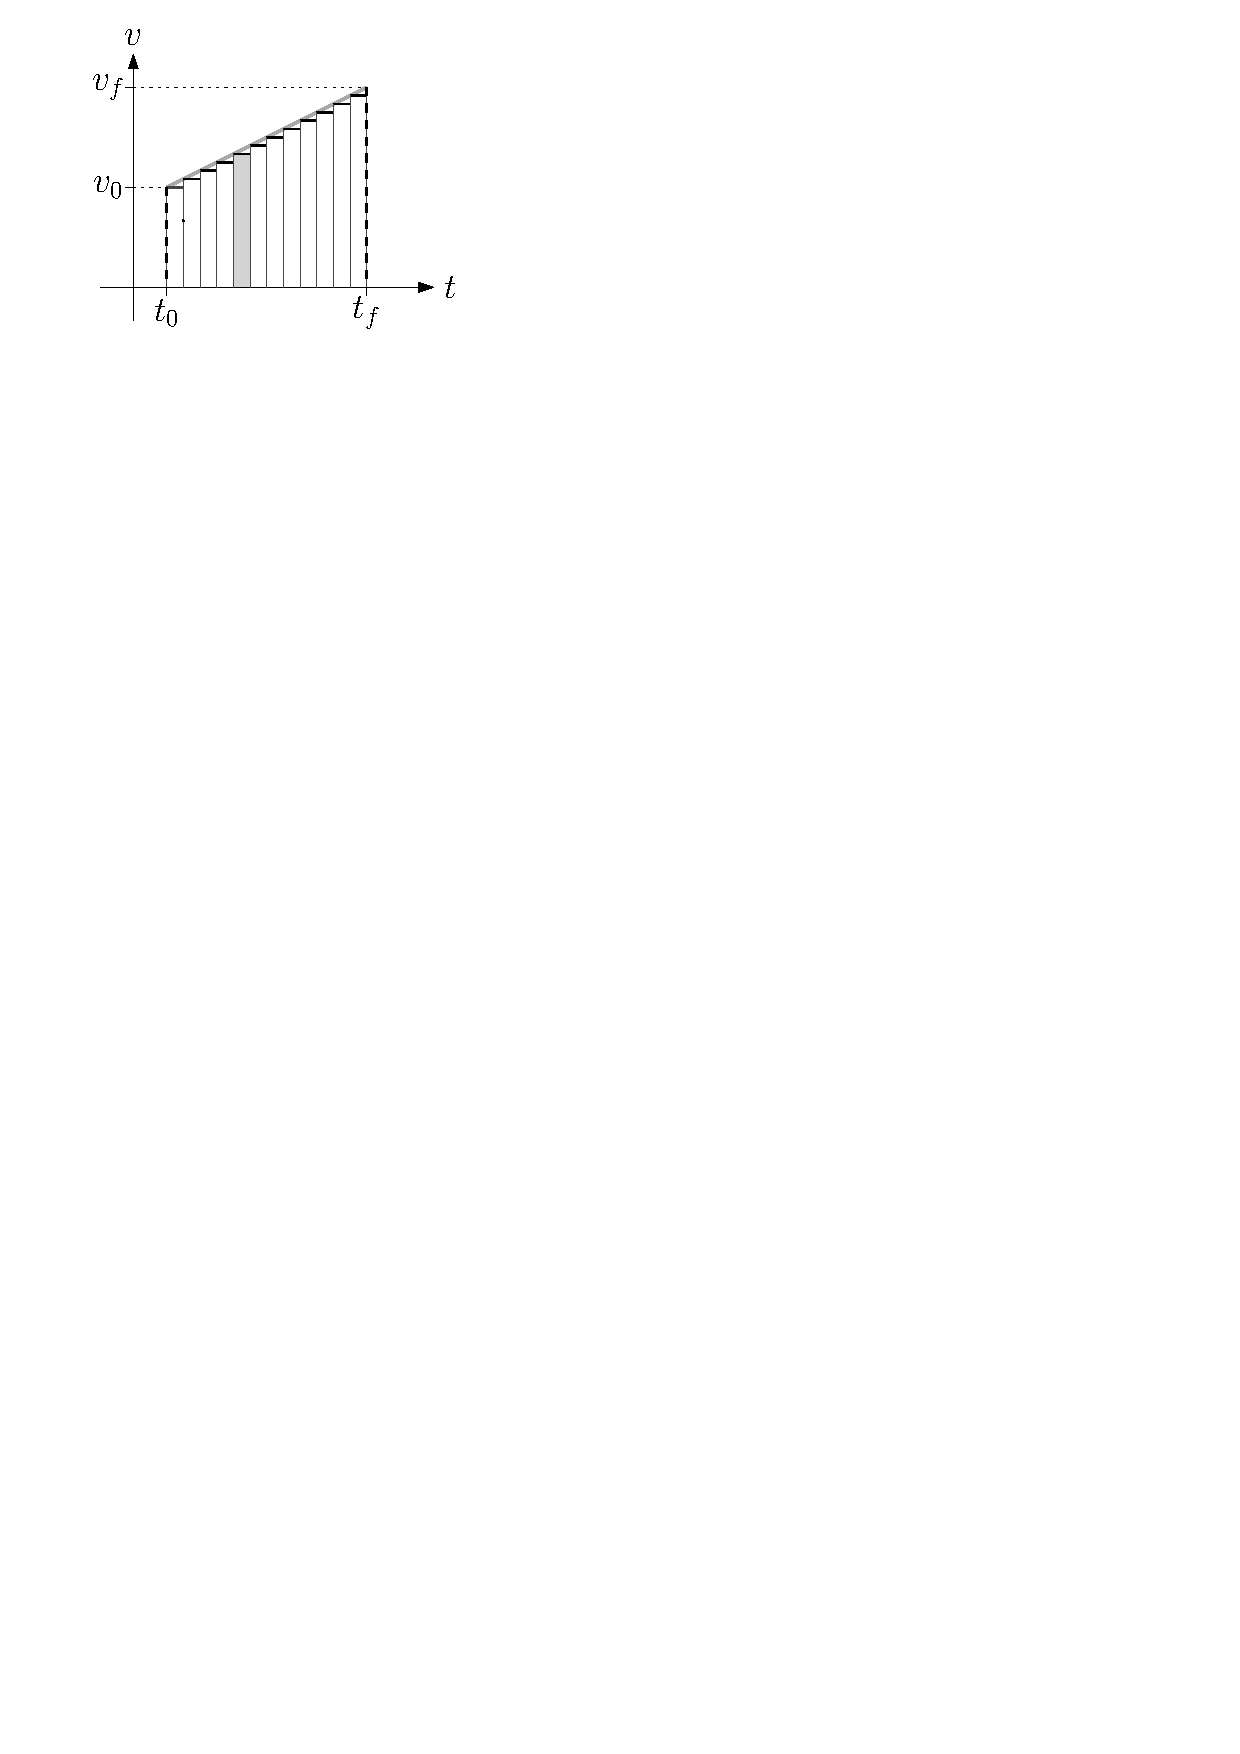
\includegraphics[scale=0.8]{img/integral.pdf}
\end{center}

Cuando la velocidad no es constante, se puede aproximar por pequeños tramos constantes. En otras palabras, podemos pensar que la partícula en cuestión se mueve con velocidad constante por pequeños intervalos de tiempo. Para cada uno de estos pequeños intervalos el desplazamiento es el área del rectángulo que queda determinado (como el que está indicado en gris en la gráfica de la Figura). Calcular el desplazamiento total equivale a sumar los desplazamientos correspondientes a cada intervalo, es decir, calcular el área bajo la curva.
\end{mybox}



Para obtener una expresión que nos permita calcular la velocidad de la partícula en función de su posición o de su desplazamiento, conociendo además su velocidad inicial y su aceleración y sin necesidad de calcular previamente el tiempo en la fórmula de posición, partimos de:
$$v = v_0 + a \Delta t$$
$$x = x_0 + v_0 \Delta t + \frac{1}{2}a(\Delta t)^2$$
Despejamos $\Delta t$ de la expresión de velocidad:
$$\Delta t = \frac{v - v_0}{a}$$
Reemplazamos en la expresión de $x$
$$x = x_0 + v_0 \frac{v - v_0}{a} + \frac{1}{2} a \frac{(v - v_0)^2}{a^2}$$
Y operando llegamos a 
\begin{center}
{\color{Magenta}  \boxed{\mathbold{v^2 = v_0^2 + 2 a \Delta x}}}
\end{center}

Vamos a ver cómo se analiza una situación de MRUV:

\begin{example}{Ejemplo}
%\item[] {\bf Ejemplo:}\\
    {\it El TGV (Train à Grande Vitesse, tren de gran velocidad, en francés) es un servicio interurbano de trenes de alta velocidad. Este tren ostenta el record de ser el tren con ruedas mas rapido del mundo, con una velocidad de $574,8 \si{km/h}$ (en condiciones de prueba). Un TGV parte de la estación, ¿cuál es la aceleración del tren, supuesta constante, si pasa de $0 \si{km/h}$ a $320 \si{km/h}$ (su velocidad operativa) en $7\si{min}$? ¿cuál es la distancia del tren a la estación a los $60\si{s}$, $120\si{s}$, $180\si{s}$ y $240\si{s}$?}
%\item[] 
    \tcblower
     {\sf {\bf Modelo:} Supondremos en este problema que el {\it TGV} es una partícula que se mueve en una trayectoria rectilínea con aceleración constante a determinar.}
  
Lo primero que hacemos es realizar un esquema de la situación física identificando los datos del problema, en este caso fijaremos el origen de coordenadas en la estación y tomaremos el sentido positivo hacia donde se mueve el tren (digamos: la derecha):
  \begin{center}
    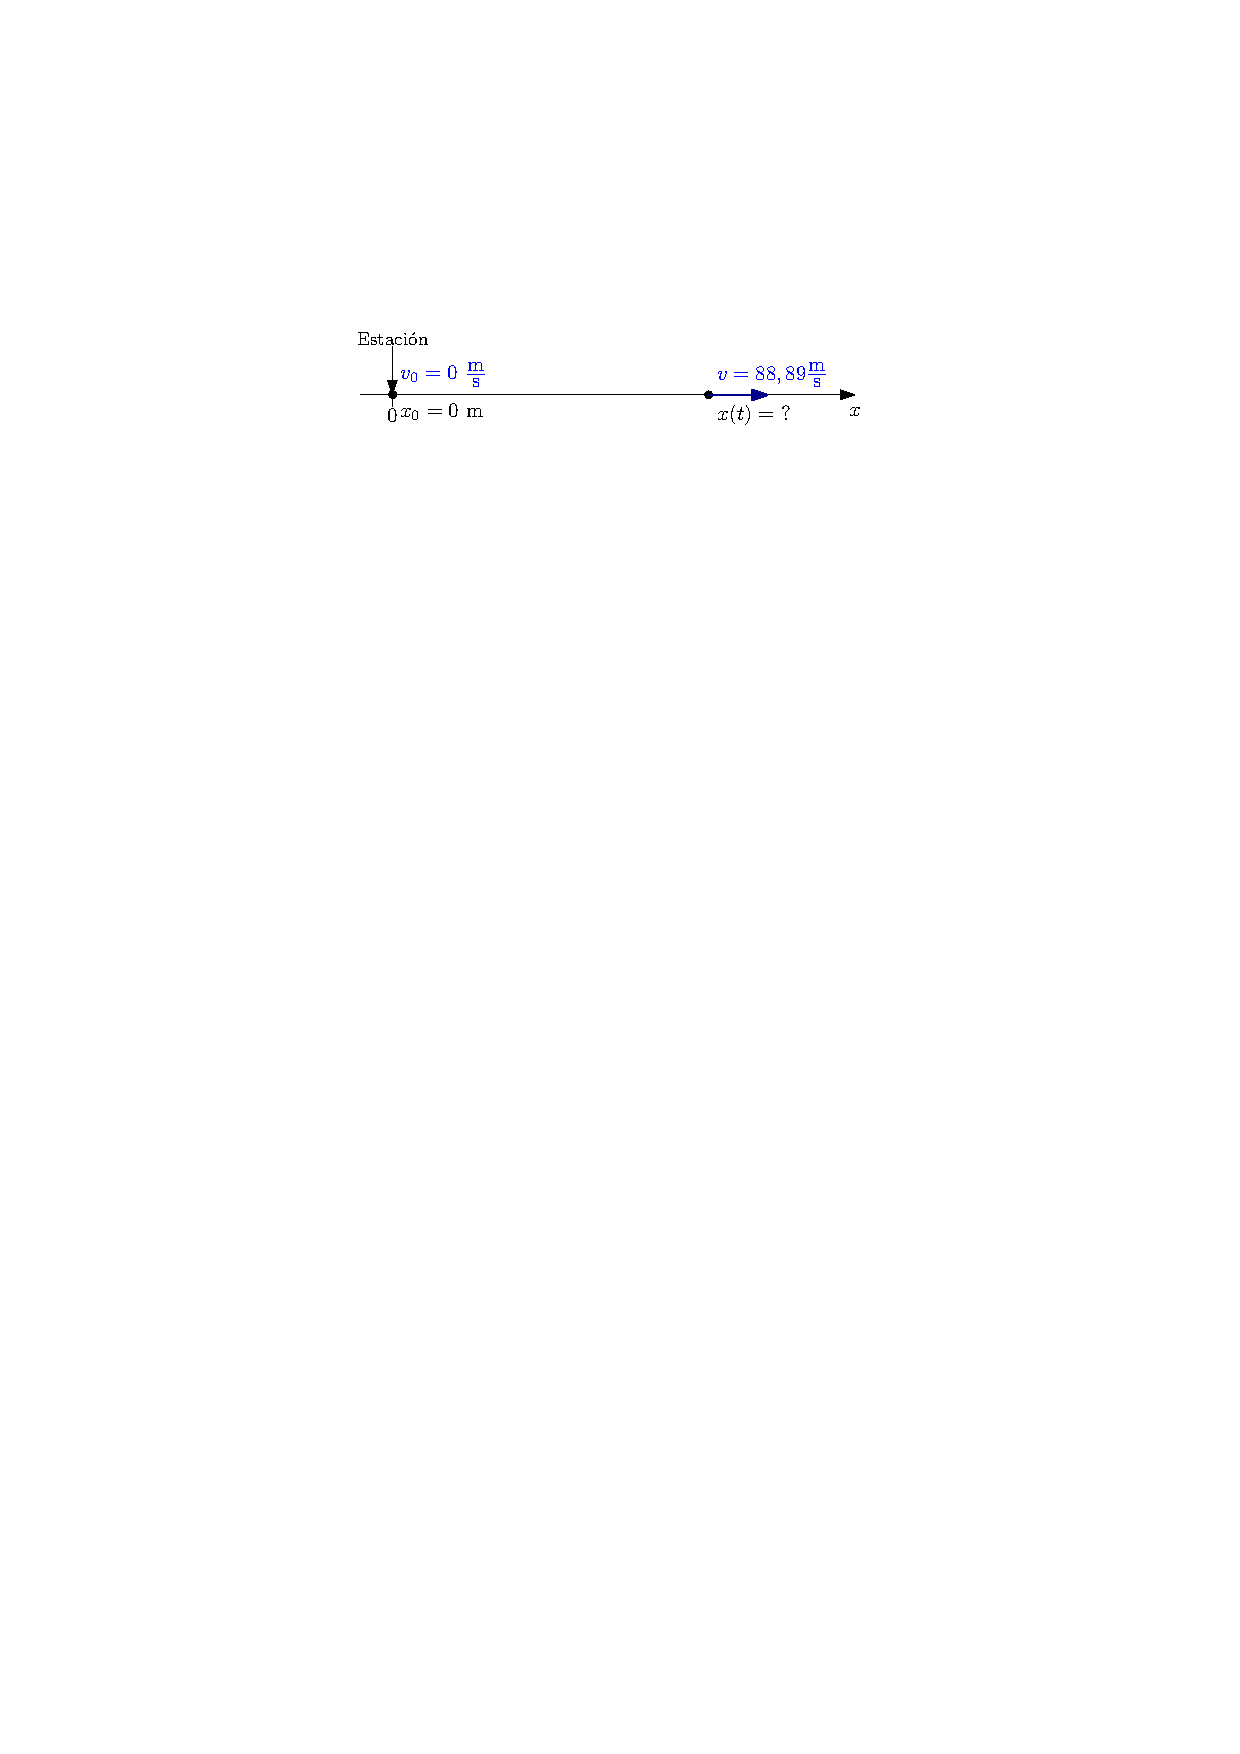
\includegraphics[]{img/tgv.pdf}
  \end{center}
  Con lo cual, podemos identificar los datos como:
  \begin{equation*}
	t_0=0\si{s}:
	\left\{
	\begin{array}{ccl}
	x_0 & = & 0\si{m}\\
	v_0 & = & 0\si{m/s}\\
	\end{array}
	\right.
	\quad
	t=7\si{min}\equiv 420 \si{s}
	\left\{
	\begin{array}{ccl}
	x & = & ?\\
	v & = & 320\sif{km}{h}\equiv 88,89 \sif{m}{s}\\
	\end{array}
	\right.
	\end{equation*}
  Nótese que dejamos indicado que la posición en el instante $t=420\si{s}$ es una incógnita. Con estos datos podemos calcular la aceleración del tren:
$$a=\frac{v-v_0}{t-t_0}=\frac{88,89\sif{m}{s}}{420\si{s}}=0,211\sif{m}{s$^2$}$$
  
  Teniendo la aceleración, podemos utilizarla junto con los datos para calcular la posición del tren respecto a la estación en los instantes pedidos (recordemos que $t_0=0\si{s}$, $x_0=0\si{m}$ y $v_0=0\si{m/s}$):
  $$60\si{s}:\quad x = \cancel{x_0} + \cancel{v_0t} + \frac{1}{2}at^2= \frac{1}{2} \cdot 0,211\sif{m}{s$^2$} \cdot (60\si{s})^2  = 379,8 \si{m}$$
  $$120\si{s}:\quad x = \cancel{x_0} + \cancel{v_0t}+ \frac{1}{2}at^2 = \frac{1}{2} \cdot 0,211\sif{m}{s$^2$} \cdot (120\si{s})^2 = 1519,2\si{m}$$
  $$180\si{s}:\quad x = \cancel{x_0} + \cancel{v_0t}+ \frac{1}{2}at^2 = \frac{1}{2} \cdot 0,211\sif{m}{s$^2$} \cdot (180\si{s})^2 = 3418,2\si{m}$$
  $$240\si{s}:\quad x = \cancel{x_0} + \cancel{v_0t}+ \frac{1}{2}at^2 = \frac{1}{2} \cdot 0,211\sif{m}{s$^2$} \cdot (240\si{s})^2 = 6076.8\si{m}$$
\end{example}

Al igual que hicimos para el MRU, la información obtenida se puede llevar a una gráfica de \textbf{posición en función del tiempo} $\mathbold{x=x(t)}$.

\begin{figure}[!h]
  \centering
  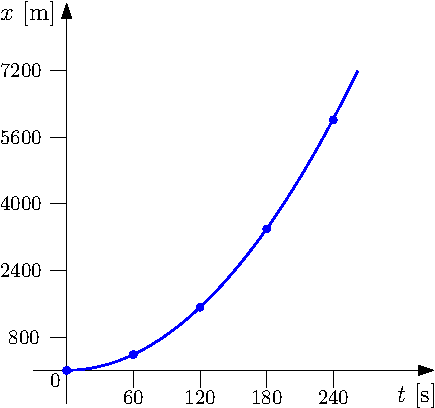
\includegraphics[scale=1]{img/x_tgv.pdf}
  \caption{\label{fig:MRUV} Gráfica típica $x=x(t)$ de un MRUV.}
\end{figure}

Se deja como ejercicio para el lector realizar la gráfica de \textbf{velocidad en función del tiempo} $\mathbold{v=v(t)}$.

La gráfica de posición en función del tiempo para un MRUV será, como en el ejemplo anterior, una \textbf{parábola}. ¿Qué información se puede extraer de este tipo de gráficas? La Figura \ref{fig:rectatangente} presenta una gráfica de posición en función del tiempo (también llamada \textbf{posición versus tiempo}, $\mathbold{x\ \mathbf{vs}\ t}$).

\begin{figure}[!h]
  \centering
  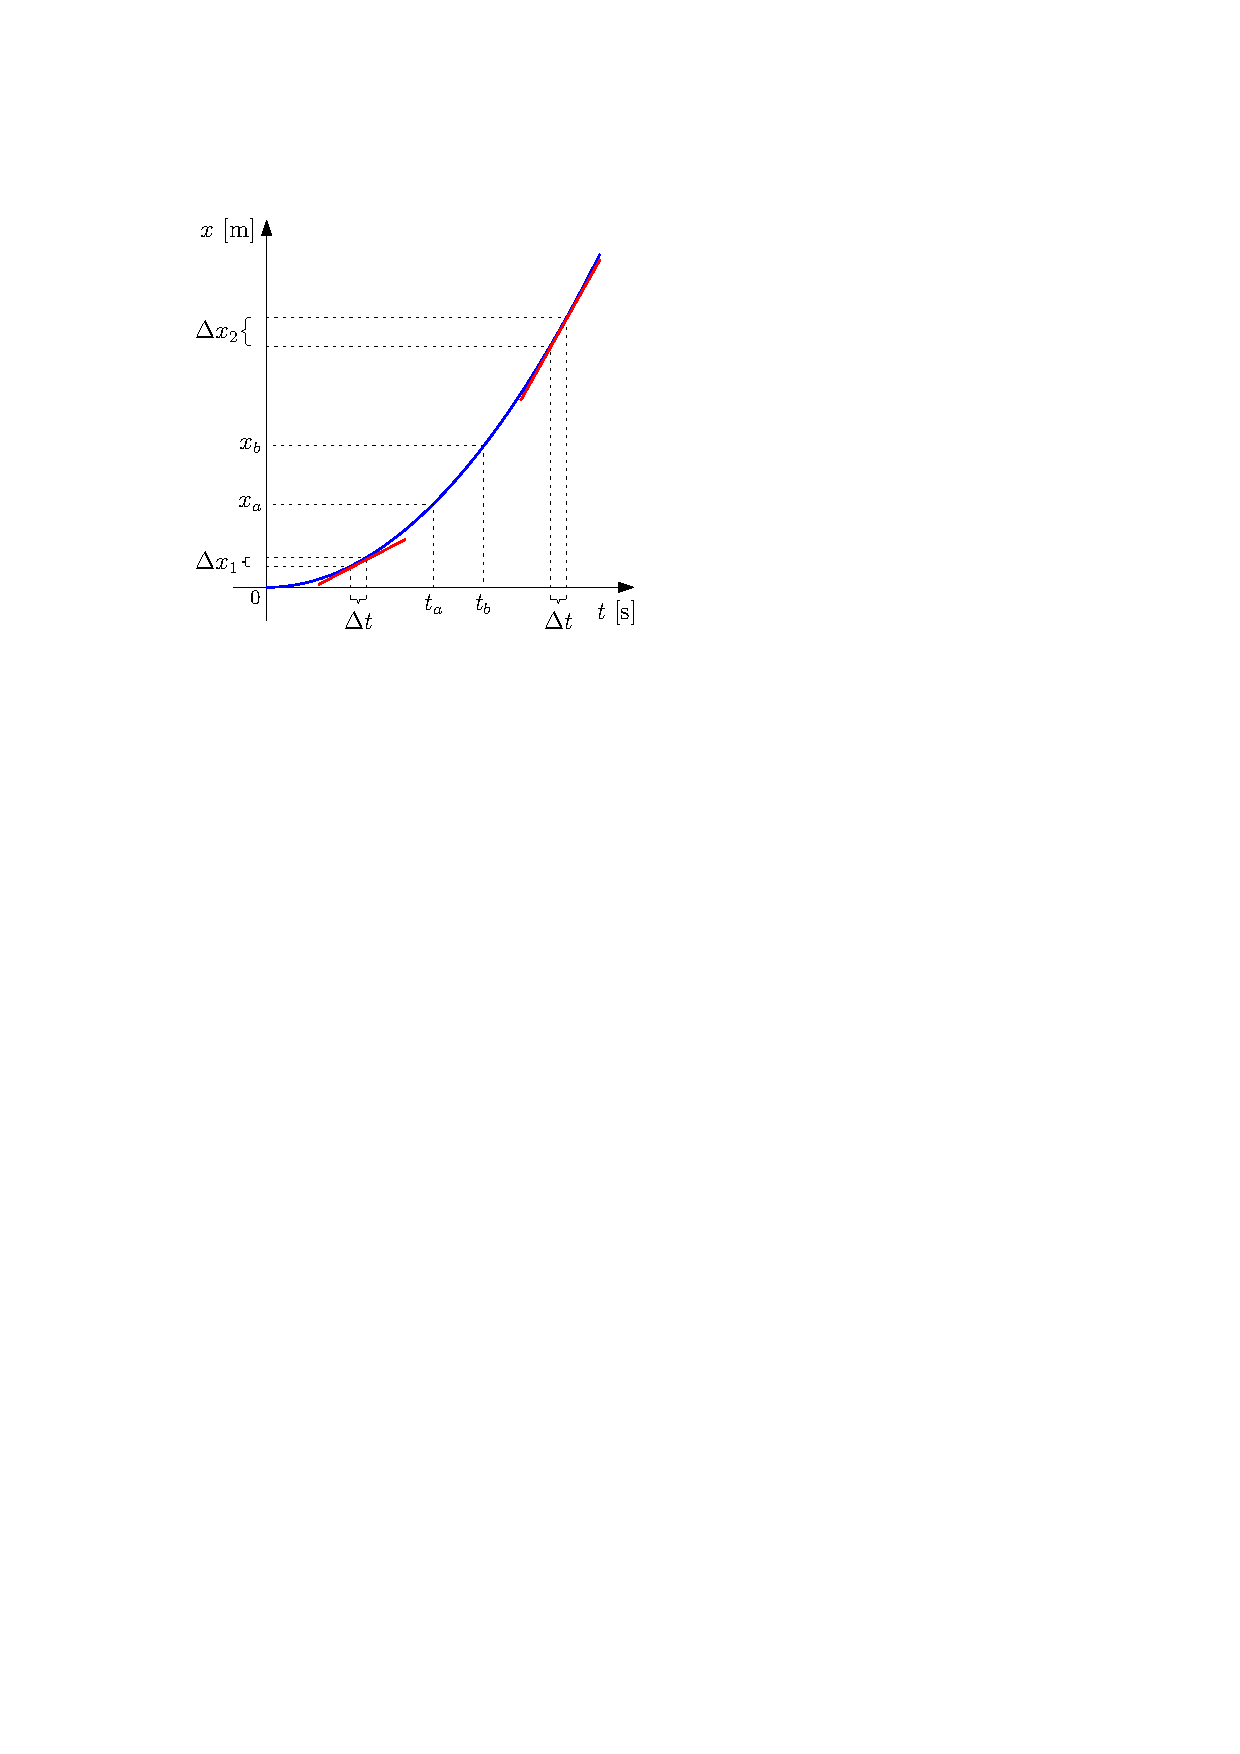
\includegraphics[scale=1]{img/rectatangente.pdf}
  \caption{\label{fig:rectatangente} Gráfica típica x=x(t) de un MRUV.}
\end{figure}

En primer lugar, podemos decir que la partícula parte de $x_0 = 0$ (ya que en $t=0$, $x=0$), y se mueve en el sentido tomado como positivo: si tomamos un instante de tiempo $t_a$ y un instante posterior $t_b$ (en el ejemplo del TGV sería por ejemplo $t_a =120\si{s}$ y $t_b=180\si{s}$), vemos que la partícula está primero en $x_a$ y luego pasa por $x_b$, y que $x_b > x_a$.

Podemos darnos cuenta que la rapidez va aumentando porque si tomamos dos pequeños intervalos de tiempo iguales (en el eje horizontal), vemos que en el intervalo que está a la derecha (es decir, que ocurre luego), el desplazamiento $\Delta x_2$ es mayor que el desplazamiento $\Delta x_1$. En otras palabras, es la pendiente de la recta tangente a la curva (en \textcolor{red}{rojo}) la que nos dice qué tan \textit{rápido} se mueve la partícula: mientras más \textit{empinada} la recta tangente, mayor es la velocidad.

A partir de la gráfica también podemos determinar que la partícula parte del reposo ($v_0=0$) ya que al principio, la recta tangente es horizontal y no tiene pendiente.

Analicemos un caso más agregando las gráficas de velocidad y aceleración en función del tiempo.

\begin{example}{Ejemplo}
%\item[] {\bf Ejemplo:}\\
    {\it Un esquiador en el Cerro Catedral (San Carlos Bariloche) desacelera hasta detenerse en una superficie horizontal luego de haber descendido por la pista. Bosquejar las gráficas de $x(t)$, $v(t)$ y $a(t)$}
%\item[] :
\tcblower
Como no tenemos más datos, fijamos un sistema de referencia arbitrario y diremos que el esquiador está en una posición inicial $x_0$ positiva cualquiera. 

  \begin{center}
    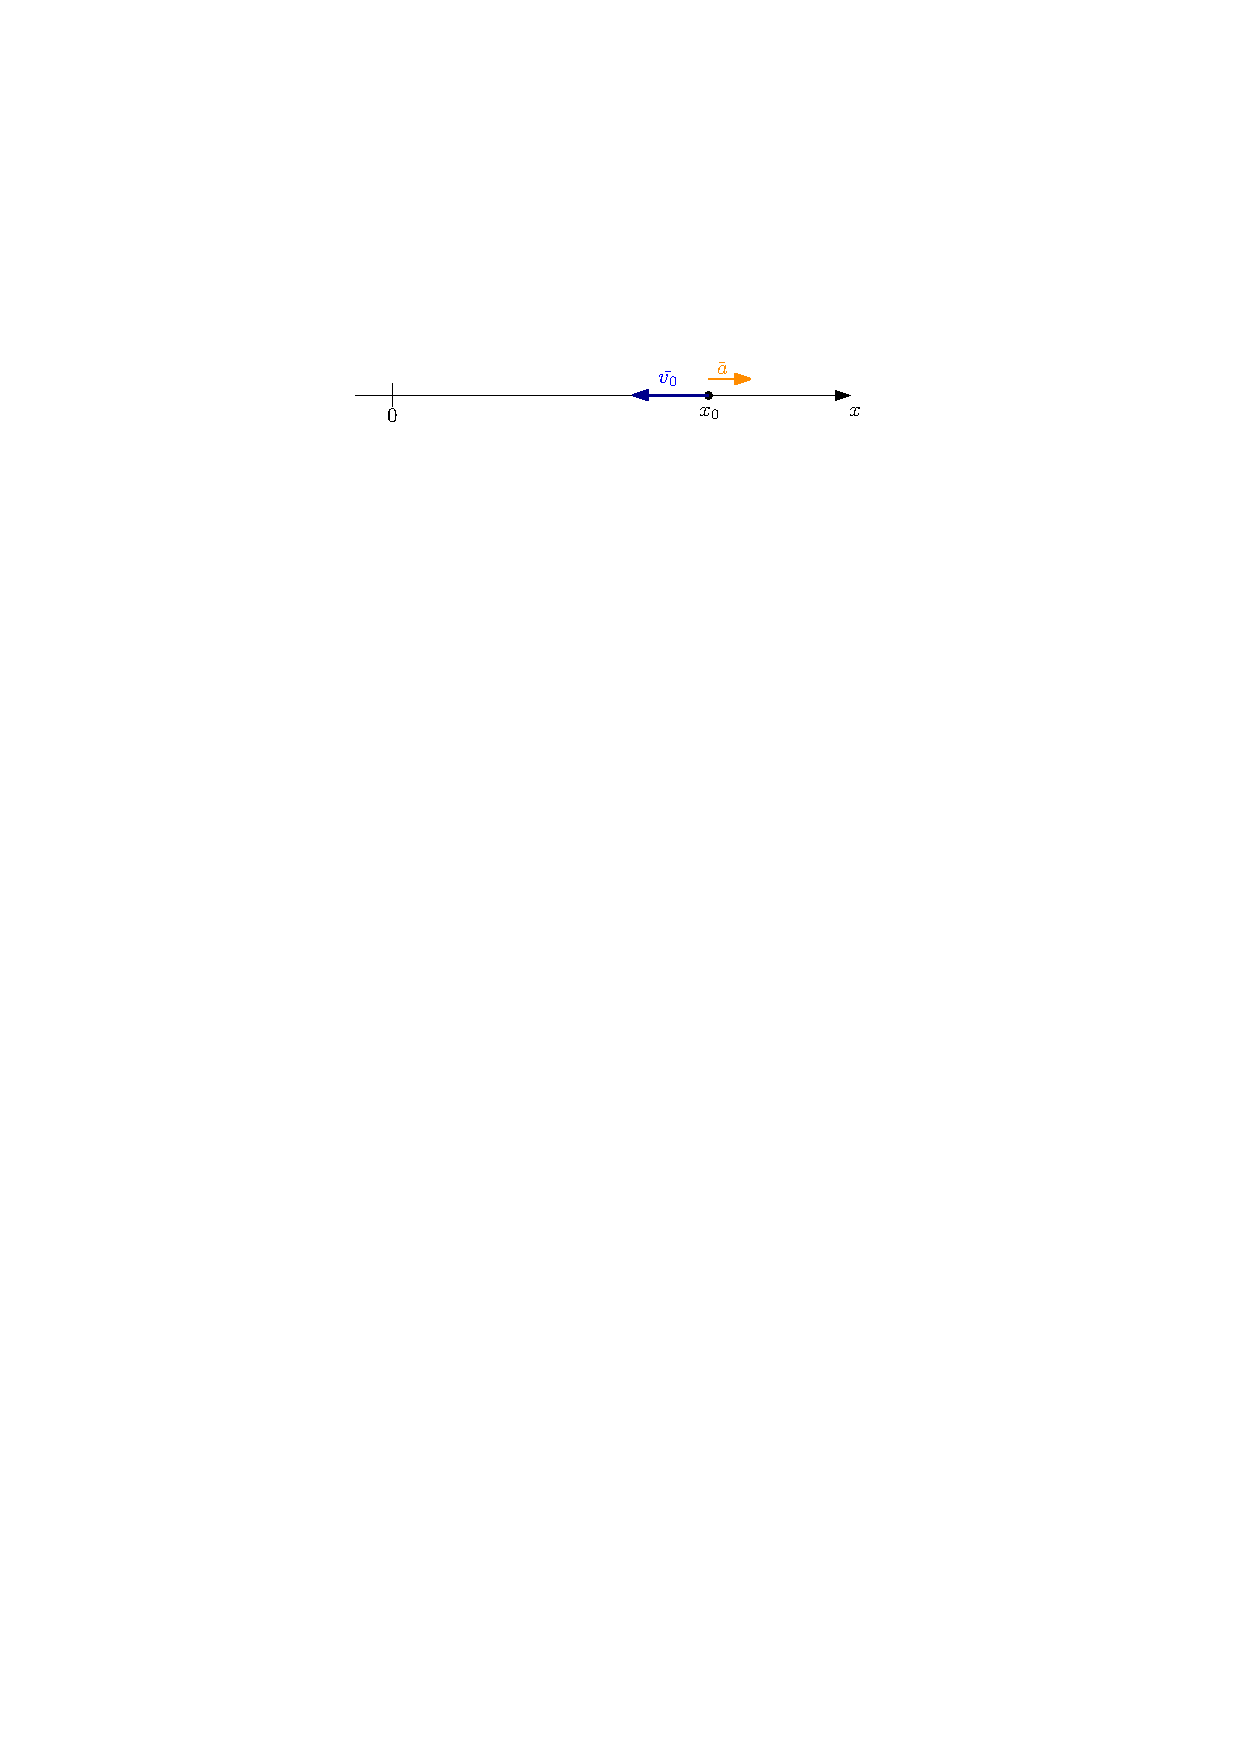
\includegraphics[]{img/esquiador.pdf}
  \end{center}

La velocidad inicial es negativa para el sistema de referencia adoptado y va hasta cero (disminuye su módulo). La aceleración es siempre positiva para el sistema de referencia. Según el esquema el esquiador se mueve acercándose al origen de coordenadas. En $t^*$ la velocidad se hace cero y el esquiador se detiene (la tangente a la curva de posición es horizontal).

  \begin{center}
    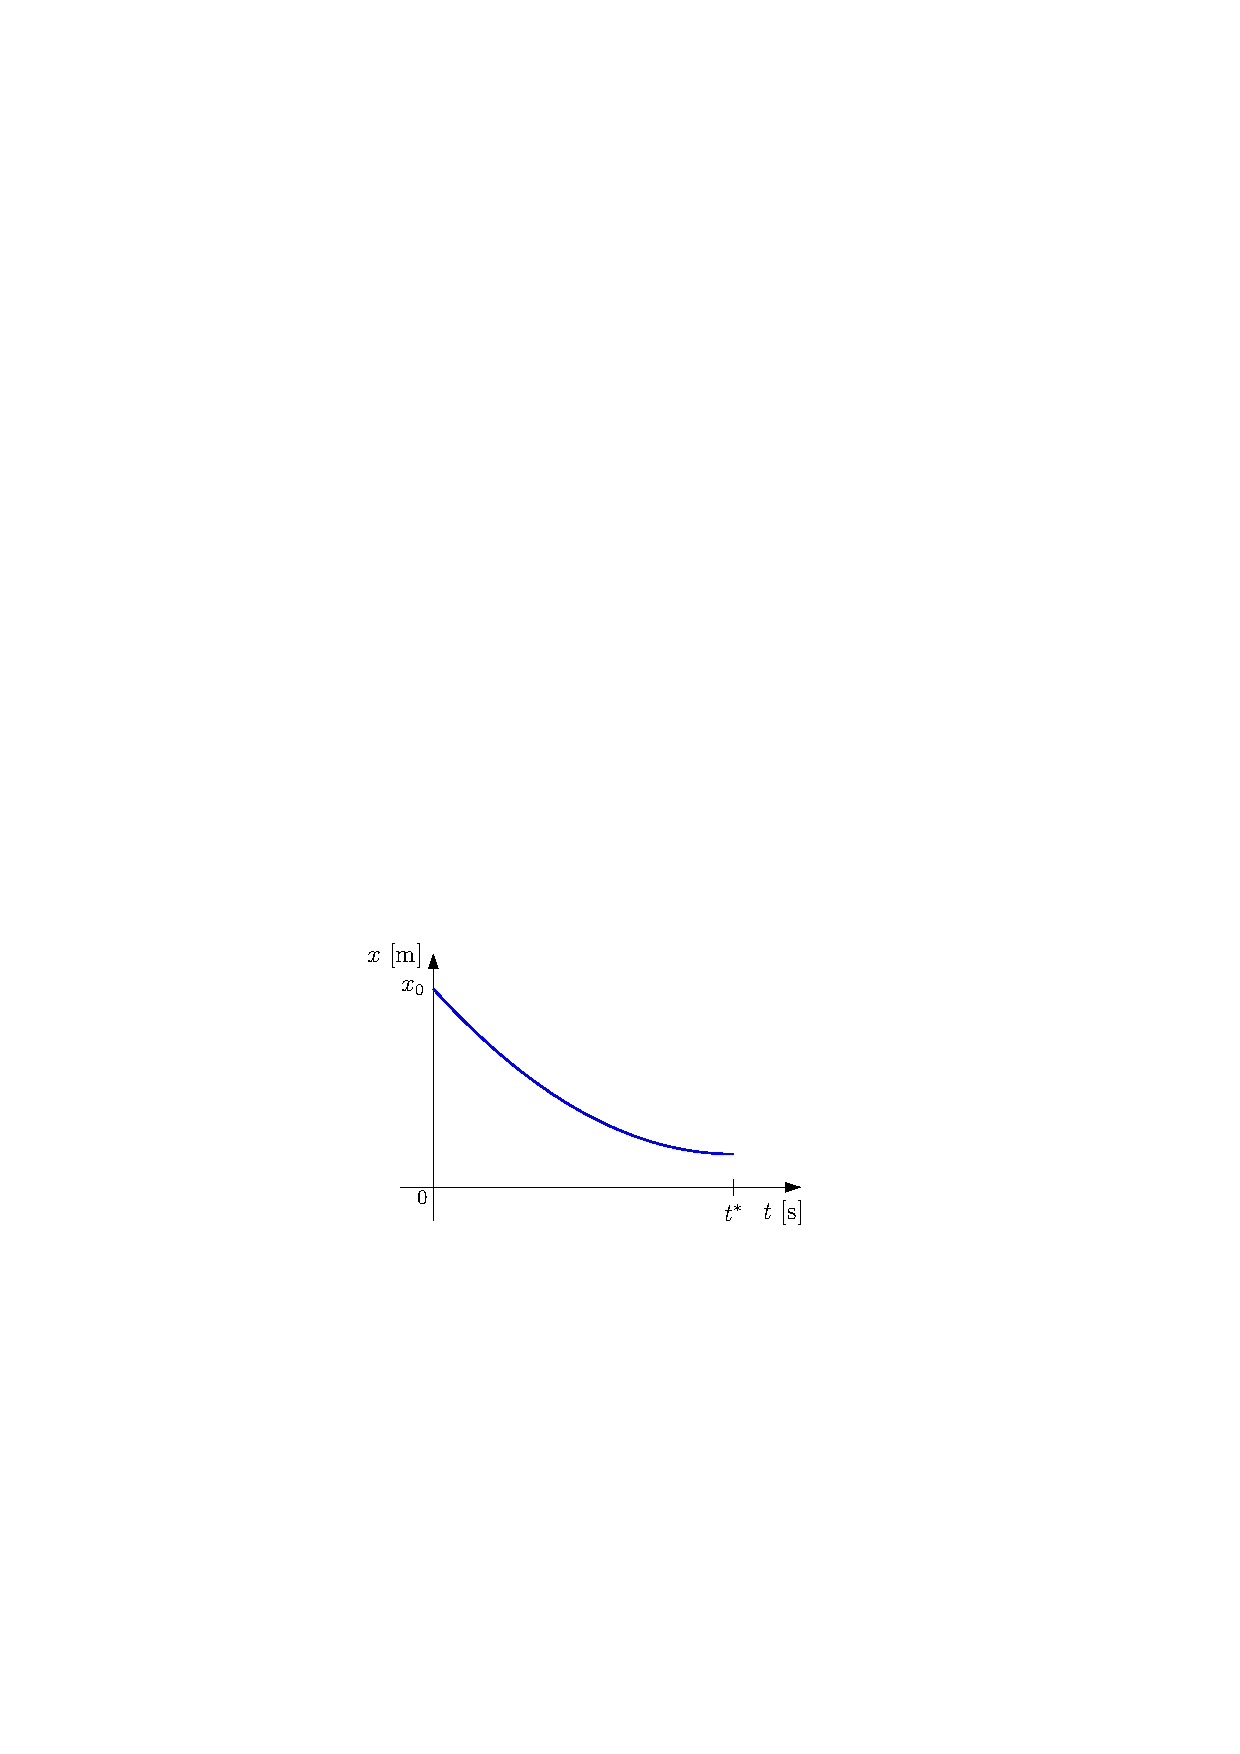
\includegraphics[]{img/plot2a.pdf}
    
    \includegraphics[]{img/plot2b.pdf}
    
    \includegraphics[]{img/plot2c.pdf}
  \end{center}
\end{example}


\begin{comprension}
  \noindent
  {\bf Primero}  Analiza las siguientes gráficas:
  \begin{center}
    \includegraphics[width=0.9\textwidth]{img/analisisMRUV.pdf}
  \end{center}

 \noindent
  {\bf Segundo} ¿Pueden la gráfica (b) y la (c) pertenecer a un mismo movimiento? ¿La (d) y la (f)? Explica.
\end{comprension}


\newpage
\section{Actividades para el aula, el laboratorio y la casa}

\subsection*{Actividad 1}
\subsubsection{Trabajo Práctico N\textordmasculine 1}


\textbf{Título:} Movimiento Rectilíneo

\textbf{Objetivo:} Describir el movimiento rectilíneo de una pequeña esfera que cae por el interior de un recipiente que contiene detergente.

\textbf{Materiales:} probeta, detergente, esferas metálicas, cronómetro,  papel milimetrado, cinta métrica.

\textbf{Procedimiento:}
\begin{itemize}
  \item Deja caer la esfera en el detergente y anticipa el tipo de movimiento que posee, según lo estudiado en cinemática.
  \item Observa que a lo largo del tubo se han hecho marcas cada 5\,cm.
  \item Planifica cómo medir el intervalo de tiempo que demora la esfera en recorrer las distancias marcadas en el papel milimetrado.
  \item Discute los procedimientos para la elección del sistema de referencia.
    \item Discute cómo reducir las incertezas que afectan a las mediciones.
\end{itemize}

\noindent
\textit{Primera Parte:}
\begin{itemize}
  \item Deja caer la esfera dentro de la probeta. Mientras la esfera desciende, mide para cada  distancia $\Delta x$ el tiempo $\Delta t$ que demora en recorrerla.
  
  \item Calcula la velocidad media  $v_{m,i}$ para cada intervalo y analiza los valores obtenidos.
  
  \item Completa la siguiente tabla:
  
  \begin{table}[!htb]
    \centering
    \label{tab:vm}
    \begin{tabular}{|c|c|c|c|c|}
    \hline
    N$^{\circ}$ & $\Delta\,x_i$ [cm] & $\Delta\,t_i$ [s] & $v_{m,i}$ [cm/s]                        & $\varepsilon \ = \ |v_{m,prom} - v_i|\si{[cm/s]}$ \\ \hline
    1           &                  &                 &                                         &                               \\ \hline
    2           &                  &                 &                                         &                               \\ \hline
    3           &                  &                 &                                         &                               \\ \hline
    4           &                  &                 &                                         &                               \\ \hline
    5           &                  &                 &                                         &                               \\ \hline
                &                  &                 & $v_{m,prom} \ = \ \frac{\sum \ v_{m,i}}{N}$ &                               \\ \hline
    \end{tabular}
    \caption{Tabla a construir en la primer parte del trabajo.}
  \end{table}
  \item Expresa correctamente el resultado de la velocidad media como $v_m \ = \ v_{m,prom} \ \pm \ \varepsilon_{max}$ (indicando unidad, dirección y sentido).
\end{itemize}

\noindent
\textit{Segunda Parte:}
\begin{itemize}
  \item Deja caer la esfera y mide el tiempo que transcurre desde el origen hasta que pasa por cada una de las posiciones marcadas.
  \item Mide las posiciones correspondientes a cada una de las marcas hechas sobre el tubo desde $x_0 \ = \ 0$\,cm.
  \item Completa la siguiente tabla:
  \begin{table}[!htb]
    \centering
    \label{tab:xvst}
    \begin{tabular}{|c|c|}
    \hline
    $x$\,[cm]                & $t$\,[s]                \\ \hline
                           &                       \\ \hline
                           &                       \\ \hline
                           &                       \\ \hline
                           &                       \\ \hline
                           &                       \\ \hline
    \multicolumn{1}{|l|}{} & \multicolumn{1}{l|}{} \\ \hline
    \end{tabular}
    \caption{Tabla a construir en la segunda parte del trabajo.}
  \end{table}
  \item Grafica $x \ = \ x(t)$.
 
  \end{itemize}


   
  Al finalizar la experimentación, confecciona un informe que contenga: título, objetivo, materiales  (indicando características de los instrumentos usados), procedimiento, observaciones, incluyendo tablas, gráficos, análisis de los resultados obtenidos y sus incertezas, y conclusiones.

  Recuerda que las conclusiones deben responder al objetivo del Trabajo Práctico, lo que en este caso implica describir todas las caracterísiticas observadas y medidas del movimiento de la bolita en el detergente. Puedes ayudarte respondiendo las siguientes preguntas: {\it ¿Se pueden aplicar algunos de los modelos estudiados en este capítulo para describir lo que ocurre con la bolita? ¿Cuáles? ¿Qué magnitudes físicas asociadas a esos modelos se pudieron identificar y medir? ¿Qué se podría decir sobre la calidad de las mediciones obtenidas? Con el equipamiento utilizado, ¿se podrían hacer mejoras al experimento? ¿Cuáles?}



%% 04 Acá van los problemas de final de capítulo, que armó Emanuel.
% %\documentclass[a4paper,11pt,draft]{article}
% %\documentclass[a4paper, 12pt]{article}
% %%%%%%%%%%%%%%%%%%%%%%%%%%%%%%%%%%%%%%%%%%%%
% %%% PAQUETES NECESARIOS
% % idioma
% \usepackage[utf8x]{inputenc}
% \usepackage[spanish]{babel}
% % figuras
% \usepackage{enumitem}
% \usepackage{graphicx, color}% Include figure files
% \usepackage{latexsym,amsfonts,amssymb, amsmath} % S\'{\i}mbolos matem\'{a}ticos
% % estilo de bibliografia
% \bibliographystyle{plain}

% % hipervinculos
% % \usepackage{hyperref}
% %%%%%%%%%%%%%%%%%%%%%%%%%%%%%%%%%%%%%%%%%%%%%%%%%
% %vertical
% \voffset=-2.5cm      % margen superior 0cm = -4.5cm
% \textheight=25cm     % alto del texto 
% \footskip=1.0cm         
% %horizontal
% \hoffset=1.0cm          
% \evensidemargin=-0.6cm  % márgen para las páginas pares
% \oddsidemargin=-0.8cm   % márgen para las páginas impares
% \marginparsep=0cm       
% \textwidth=16.5cm       % ancho del texto
% \linespread{1.2}        % interlineado 
% %%%%%%%%%%%%%%%%%%%%%%%%%%%%%%%%%%%%%%%%%%%%%%%%%
% %%% INICIO DEL DOCUMENTO


% \begin{document}
% \renewcommand{\tablename}{Tabla}
% \title{Problemas}
% \maketitle

\subsection*{Actividad 2}
\subsubsection{Resuelve los siguientes problemas}

\begin{enumerate}
\item Desde la terraza de un edificio de 24 m de altura se arroja verticalmente hacia arriba una pelota. Esta sube 1,4 m y luego cae a la vereda, rebota 80 cm y es atrapada por una persona.
  \begin{enumerate}
  \item Realiza un esquema de la situación.
  \item Representa el desplazamiento y calcula su módulo.
  \item Calcula la distancia recorrida por la pelota.
  \end{enumerate}
  \resp{Distancia recorrida = 27,60 m; $\bar{d}$ = \{vertical, descendente, 23,20 m\}.}
    
  \item ¿Cuál es el desplazamiento de un coche que viaja por una ruta rectilínea a una velocidad media de 40\,km/h hacia el norte durante 22\,min?
      \resp{$\Delta \bar{x}$ = \{dirección la recta en la que se mueve, sentido hacia el norte, 14,66\,km\}.}

  \item ¿A qué distancia se encuentra  la estrella  ``61 del Cisne'' si su luz necesita 11 años para llegar a la Tierra? \href{http://www.elmundo.es/elmundo/2009/06/08/ciencia/1244457000.html}{Esta distancia fue descubierta por Bessel en 1838 \faExternalLink}. Ten en cuenta que la luz tiene una rapidez en el vacío  $c = 3 \times 10^8$\,m/s.
    \resp{$Dist = 1.04 \times 10^{14}$\,km}

  \item \href{https://www.youtube.com/watch?v=ObuWeZNdem4}{La nebulosa ``Cabeza de Caballo'' \faExternalLink} es una nebulosa oscura en la constelación de Orión, descubierta por la astrónoma escocesa \href{https://elpais.com/elpais/2015/10/28/ciencia/1446051155_519282.html}{Williamina Fleming \faExternalLink} en 1888 aunque, inicialmente, no recibió crédito por ello. Esta masa de gas oscura contrasta con la brillante nebulosa IC434 que la rodea. Ambas masas de gas y polvo interestelar se hallan aproximadamente a $1.42\times 10^{19}$\,m de la Tierra. Calcula el tiempo {\it en segundos y en años} que tardaría un rayo de luz proveniente de esa región del espacio en alcanzar nuestro planeta.
    \resp{$\Delta t = 4.733 \times 10^{10}\si{s} \approx 1500\si{años}$ }
  
  \item Se usa un cronómetro para tomar el tiempo de un automóvil en movimiento sobre una pista rectilínea y horizontal. En el tiempo $t =  12$\,s, el automóvil está en $x =  50$\,m. En  $t =  15$\,s, el automóvil está en $x =  5$\,m. ¿Cuál es la velocidad media y cuál es la rapidez media del automóvil?
      \resp{$\bar{v}_m \ = $ \{horizontal, izquierda, 15 m/s\}; $|\bar{v}_m| =  15$\,m/s}
  
  \item Una mujer conduce desde el lugar $A$ hasta el lugar $B$ por un camino recto. Durante los primeros 75\,min conduce a una rapidez media de 90\,km/h. Para, entonces, durante 15\,min. Continúa su viaje conduciendo a una rapidez de 75\,km/h durante 45\,min. A continuación conduce a 105\,km/h durante 2,25\,h y llega a su destino. Calcula la velocidad media entre $A$ y $B$.
      \resp{$\bar{v}_m \ = $ \{en la recta que une $A$ y $B$, desde $A$ hacia $B$, 90\,km/h.\}}
  
  \item Un automóvil va a 72\,km/h por un camino recto durante $\frac{1}{2}$ minuto. Grafica $v =  v(t)$ y $x =  x(t)$ para dicho intervalo.
  
  \item En un tramo recto de una carretera un automóvil lleva una velocidad uniforme de 70\,km/h. Detrás de éste y a 35\,km de distancia otro automóvil avanza con velocidad uniforme de 110\,km/h. ¿En cuánto tiempo alcanza éste al primero, suponiendo que mantienen el movimiento rectilíneo y uniforme?\\
  Además de encontrar el resultado analíticamente, realiza los gráficos posición -- tiempo de ambos móviles.
\resp{$t_{encuentro} =  0,875\,$h $\equiv \ 52,5$\,min.}
  
  \item Cada uno de los siguientes cambios de velocidad tienen lugar en un intervalo de tiempo de 10\,s y mientras la partícula en movimiento se desplaza sobre un eje horizontal. Determina la dirección, el sentido y el valor de la aceleración media para cada intervalo, recuerda que se trata de una magnitud vectorial. Indica en cada caso si el movimiento es acelerado o desacelerado.
  \begin{enumerate}[label=\alph*)]
    \item Al comienzo del intervalo se mueve hacia la derecha con velocidad inicial $v ~ = ~ 150$\,cm/s y al final del mismo la velocidad es $v =  600$\,cm/s hacia la derecha.
    \item Al comienzo hacia la derecha con $v =  600$\,cm/s y al final hacia la derecha con $v =  150$\,cm/s.
    \item Al comienzo hacia la izquierda con $v =  600$\,cm/s y al final hacia la izquierda con $v =  150$\,cm/s.
    \item Al comienzo hacia la izquierda con $v =  150$\,cm/s y al final hacia la izquierda con $v =  600$\,cm/s.
    \item Al comienzo hacia la izquierda con $v =  150$\,cm/s y al final hacia la derecha con $v =  600$\,cm/s.
  \end{enumerate}
  
  \item Un trineo parte del reposo descendiendo por una ladera con una aceleración constante de 2\,m/s
  \begin{enumerate}[label=\alph*)]
    \item ¿Qué velocidad lleva al cabo de 5\,s?
    \item ¿Qué distancia recorre en 5\,s?
    \item ¿Cuál es la velocidad media durante los primeros 5\,s?
    \item ¿Qué distancia ha recorrido hasta el instante en que su velocidad alcanza los 40\,m/s?
    \item Grafica $a\ =\ a(t)$, $v =  v(t)$ y $x =  x(t)$.
  \end{enumerate}

  \resp{
 a) $\bar{v}(5s) \ = $ \{la inclinación de la ladera, hacia abajo, 10\,m/s\};\,  b) $Dist|_{t\,=\,5\,s} =  25$\,m;\\
 c) $\bar{v}_m \ = $ \{la inclinación de la ladera, hacia abajo, 5\,m/s\};\,  d) $Dist|_{v\,=\,45\,m/s} =  400$\,m}

\item Un coche que inicialmente se mueve con velocidad constante acelera a razón de 1\,m/s durante 12\,s. Si en ese tiempo recorre 190\,m, ¿cuál era la lectura en el velocímetro cuando comenzó a acelerar?
  \resp{$v_0 =  9,83$\,m/s $\equiv \ 35,39$\,km/h}

  \item Un tren parte del reposo de una estación y acelera durante 1\,min con una aceleración constante de 1,2\,m/s. Después marcha a velocidad constante durante 2\,min y luego desacelera a razón de 2,4\,m/s hasta que se detiene en la estación siguiente.
  \begin{enumerate}[label=\alph*)]
    \item Calcula la distancia total recorrida por el tren.
    \item Grafica $a =  a(t)$, $v =  v(t)$ y $x =  x(t)$.
  \end{enumerate}
  \resp{$Dist =  11,88$\,km}
  
   
  \item \label{prob:11} ¿V o  F?: ``Las gráficas de la Figura~\ref{fig:prob11} corresponden a un MRUV para un móvil que estando a 8\,m a la derecha del origen, desacelera hasta detenerse, moviéndose en sentido opuesto al elegido como positivo sobre el eje de referencia''

\begin{figure}[!htb]
      \centering
      \includegraphics[width=0.8\textwidth]{img/prob11.pdf}
      \caption{\label{fig:prob11} Problema \ref{prob:11}}
  \end{figure}
    

\item \label{prob:12} La gráfica de la Figura~\ref{fig:prob12} corresponde a la velocidad en función del tiempo de un movimiento rectilíneo.
  
  \begin{figure}[!htb]
    \centering
    \includegraphics[scale=0.8]{img/prob12.pdf}
    \caption{\label{fig:prob12} Problema \ref{prob:12}}
  \end{figure}
  
  Calcula:
  \begin{enumerate}
    \item Distancia recorrida y valor del desplazamiento a los 12\,s.
    \item Velocidad media en [0; 12]\,s.
    \item Velocidad a los 5\,s.
  \end{enumerate}
  Grafica:
  \begin{enumerate}
    \item $a =  a(t)$ en [0; 12]\,s.
    \item $x =  x(t)$ en [0; 12]\,s.
  \end{enumerate}

  \resp{a) $Dist|_{t\,=\,12\,s} =  138$\,m y $\Delta \bar{x} \ = $ \{horizontal, hacia la derecha, 54\,m\}; \, b) $\bar{v}_m\ = $ \{horizontal, hacia la derecha, 4,5\,m/s\};\, c) $\bar{v}(5\,s)\ = $ \{horizontal, hacia la derecha, 12\,m/s\}.}

  \item Un vehículo viaja a 90\,km/h cuando el conductor ve un animal en la carretera 40\,m adelante. Si el tiempo de reacción del conductor es de 0,48\,s (aplica los frenos 0,48\,s después de ver el animal), y la desaceleración máxima de los frenos es de 7,6\,m/s$^2$ ¿El automóvil se detendrá antes de chocar al animal?
  
  \item Un electrón tiene una velocidad inicial de $3 \times 10^5$\,m/s. Si experimenta una aceleración de $8 \times 10^{14}$\,m/s$^2$, ¿cuánto tardará en alcanzar una velocidad de $5.4 \times 10^5$\,m/s? y ¿qué distancia recorre en este tiempo?
  \resp{$t  =  3 \times 10^{-10}$\,s; $Dist  =  1.26 \times 10^{-4}$\,m.}

  \item Dos amigos se ven cuando están a una distancia de 160\,m y corren a encontrarse. Uno corre a 10\,m/s y el otro a 7,5\,m/s. ¿Qué distancia recorre cada uno hasta encontrarse?
\resp{$Dist_{A1} =  91,43$\,m; $Dist_{A2} =  68,57$\,m}

  \item Un auto marcha a una velocidad de 80\,km/h en una zona escolar. Un coche de policía se pone en marcha en el momento en que el auto pasa junto a él y acelera de un modo constante a razón de 8\,km/h-s (2,2\,m/s$^2$).
  \begin{enumerate}[label=\alph*)]
  \item Grafica $x$ vs. $t$ para ambos coches.
    \item ¿Cuándo alcanza el coche de policía al auto?
    \item ¿Con qué rapidez irá el coche de policía en ese momento?
  \end{enumerate}
   \resp{b) $t_{encuentro} =  20$\,s; c) $|\bar{v}_{encuentro}|\ = $ 160\,km/h.}

  \item
  \begin{enumerate}
    \item Un automóvil frena hasta detenerse con una desaceleración uniforme $a$ en un tiempo $t$. demuestre que la distancia recorrida durante ese tiempo está dada por $\displaystyle x =  \frac{v^2}{2a}$  donde $v$ es la velocidad inicial y la dirección positiva se toma en sentido del movimiento inicial.
    \item Si  su velocidad inicial es de 90\,km/h y su aceleración es 5\,m/s$^2$, ¿qué distancia recorre hasta detenerse?
    \item Si ahora la velocidad inicial es de 180\,km/h, calcule la nueva distancia de frenado y compare con el valor anterior (es mayor o menor, es el doble, el triple, etc.)
    \item A partir de la expresión obtenida en a), trate de deducir qué ocurre con la distancia de frenado cuando se duplica la velocidad inicial.
  \end{enumerate}

  \item Un electrón en un tubo de rayos catódicos de un televisor entra en una región con velocidad $v_0$ y acelera de manera uniforme hasta una rapidez $v$ en una distancia $d$. Si la dirección del movimiento es a lo largo del eje x.
  \begin{enumerate}
    \item Demuestre que la expresión para calcular el tiempo que el electrón está en la región donde se acelera es $\displaystyle t =  \frac{2 d}{v_0 \ + \ v}$.
    \item Si la velocidad inicial del electrón es de $3 \times 10^4$\,m/s, su velocidad final es de $5 \times 10^6$\,m/s y recorre una distancia de 2\,cm. ¿Durante cuánto tiempo el electrón se acelera?
  \end{enumerate}

  \item Juan y Ana hicieron un viaje de Rosario a Santa Fe. Ana fue la mitad de la distancia a velocidad $v_1$ y la otra mitad a velocidad $v_2$. Juan en cambio, fue la mitad del tiempo a velocidad $v_1$ y la otra mitad a velocidad $v_2$. Si $v_1 =  2\,v_2$ y los dos salieron juntos de Rosario ¿Quién llegó antes? ¿Por qué?

  \item Una persona camina a través de una habitación de tal modo que, después de haber iniciado el movimiento, su velocidad es negativa pero su aceleración es positiva.
  \begin{enumerate}
    \item ¿Cómo sigue esto?
    \item Realiza un gráfico $v =  v(t)$ para este movimiento.
  \end{enumerate}
\end{enumerate}


\begin{thebibliography}{99}
\bibitem{f0} {``Física 1''; Maiztegui A P, Sábato J, Kapelusz; 2da ed., Buenos Aires, 2005}
\bibitem{01} {``Movimiento en una dimensión''; Grigioni L, Palmegiani M, Schafir A; Instituto Politécnico Superior, UNR, Rosario, 2017}
  \bibitem{02} {``Física''; M. Alonso, E. J. Finn; Addison--Wesley Iberoamericana, Estados Unidos,1995}
  \bibitem{f1} {``Física''; Wilson J, Buffa A, Lou B; Prentice Hall Inc., México, 2007}
  \bibitem{f2} {``Física para la Ciencia y la Tecnología''; Volumen 1; Tipler P, Editorial Reverté, España, 2001}
  \bibitem{f3} {``Fundamentos de Física'', Volumen 1; Serway R, Faughn J; 6ta ed., International Thomson Editores, México, 2004}
  \bibitem{f4} {``Física. Conceptos y aplicaciones''; Tippens P; Mc Graw Hill, México, 2001}
  \bibitem{f5} {``Física''; Wilson J; Prentice Hall Hispanoamericana, México, 1996}
  \bibitem{f6} {``Física''; Blatt F; Prentice Hall Hispanoamericana, México, 1991}
  \bibitem{f7} {``Física'', Tomo 1; Serway R; Mc Graw Hill, México, 1997}
  \bibitem{f8} {``Física. Principios y aplicaciones''; Giancoli D; Editorial Reverté, España, 1985}
  \bibitem{f9} {``Física EGB 3''; Reynoso L; Editorial Plus Ultra, Brasil, 1998}
  \bibitem{f10} {``Física General''; Alvarenga B,  Máximo A; Editorial Harla, México, 1981}
  \end{thebibliography}
  \thispagestyle{empty}


%\end{document}


\end{document}
